\chapter[$pp\rightarrow\W\rm{H}$]{Search for the Higgs boson in tau decays in the process $pp\rightarrow\W\rm{H}$}%Search for a Standard Model Higgs boson in association with a W}

As described in Chapter 1, the Higgs boson is produced at the LHC via three main processes: the gluon fusion (GF), the vector boson fusion (VBF) and the associated production (AP). Even though the associated production has a production cross section one order of magnitude smaller than the dominant gluon fusion, the presence of an additional high-\pT lepton enhances the signal over background ratio. 
%Moreover, the associated production is a promising channel to measure the tau Yukawa coupling once enough integrated luminosity will be collected. \bold{ TODO: I STILL HAVE TO EXPLAIN WHY}

In this chapter we describe the search for the associated production of a W and a Higgs boson, where the W boson decays into a light lepton (electron or muon, generically denoted as $\ell$ from now on) and a neutrino, and the Higgs boson decays into a tau pair, with one tau decaying leptonically. Three final states are considered: $\mu\mu\tau_h$, $e\mu\tau_h$ and $ee\tau_h$. 

\section{Event Selection}

Events are selected in real time by the double lepton triggers, requiring either two muons, two electrons or a muon and a electron. The changing running conditions and increasing instantaneous luminosity required a tuning of the trigger object requirements in order to meet the constraints in bandwidth. Trigger paths, i.e. the ensemble of the selections for a certain type of trigger, having a excessive acceptance rate have been suppressed by randomly sampling them (a procedure called \emph{prescale}).

The unprescaled triggers with the lowest \pT thresholds available for each running period have been chosen. This choice results in \pT thresholds ranging from 7 up to 17 GeV and from 7 to 8 GeV for the leading and sub--leading muons in the double muon trigger. The \pT thresholds in muon plus electron and double electrons have been kept constant at 17 GeV for the leading object and 8 GeV for the sub--leading one, but electrons underwent a progressively tighter selection according to their isolation value. Further description of the electrons and muons objects computed at trigger level can be found in \cite{Chatrchyan:2012xi,CMS-PAS-EGM-10-004}.

During offline analysis, leptons are selected according two criteria called ``loose'' and ``tight''. The distinction between loose and tight leptons is used to model the irreducible background as will be described in the following sections. 

\begin{itemize}
\item Loose muons are required to:
\begin{itemize}
\item be reconstructed as global or tracker muons;
\item have $\pt > 10$ GeV, $|\eta| < 2.4$, $|d_Z| < 0.2$ cm;
\item include at least one hit in the pixel detector, to discriminate against in--flight decays;
\item the jet closest to the muon should not pass the loose $b$-tagging discriminator, to reject $t\anti{t}$ events
\end{itemize}

\item Loose electrons are required to:
\begin{itemize}
\item have $\pt > 10$ GeV, $|\eta| < 2.5$, $|d_Z| < 0.2$ cm;
\item have no missing tracker hits; 
\item have ``tight'' charge agreement, i.e. the charge measured by the CTF, the GSF and the pixel-only algorithm should agree. This requirement reduces the electron charge mis-identification;
\item the jet closest to the electron should not pass the loose $b$-tagging discriminator, to reject $t\anti{t}$ events
\end{itemize}

\item Loose taus are required to:
\begin{itemize}
\item have $\pt > 20$ GeV, $|\eta| < 2.3$, $|d_Z| < 0.2$ cm;
\item pass the ``decay-mode finding'' discriminator \ref{sec:tau_id}; 
\item not overlap with any electron passing loose MVA identification and with $Iso_{rel} < 0.3$ with \db correction in a cone of radius $\Delta R < 0.4$.
\end{itemize}

\end{itemize}

Offline event selection is different for the three channels and is detailed in the following sections:

\subsubsection{$\mu\mu\tau_h$}
\begin{itemize}
\item The event must pass the lowest--threshold unprescaled double muon trigger;
\item Both the muons must be matched to the corresponding trigger candidates;
\item The leading muon must have $\pt > 20$ GeV, to be compliant with the online thresholds;
\item Both muons must pass the PF Tight identification working point;
\item The leading muon $\Delta \beta$-corrected relative PF isolation in a cone of $\Delta R < 0.4$ has to be less than 0.15 (0.1) for candidates with $|\eta| < 1.479$ ($|\eta| > 1.479$);
\item The sub-leading muon $\Delta \beta$-corrected relative PF isolation in a cone of $\Delta R < 0.4$ has to be less than 0.2 (0.15) for candidates with $|\eta| < 1.479$ ($|\eta| > 1.479$);
\item The hadronic tau candidate is required to pass the loose isolation working point to suppress the backgrounds with jets misidentified as $\tau_h$, the loose electron rejection working point and the tight muon rejection working point to suppress the background process $\Z\To\mu\mu+\rm{jet}$ where a muon is misidentified as the hadronic tau and the jet as a muon.;
\end{itemize}

\subsubsection{$e\mu\tau_h$}
\begin{itemize}
\item The event must pass the lowest--threshold unprescaled muon plus electron trigger;
\item Both the electron and the muon must be matched to the corresponding trigger candidates;
\item The muon is required to have $\pt > 20$ GeV if the trigger accepting the event has a 17 GeV threshold on the muon candidate;
\item The electron is required to have $\pt > 20$ GeV if the trigger accepting the event has a 17 GeV threshold on the electron candidate;
\item The electron is required to pass the ``loose'' MVA identification working point;
\item The electron $\Delta \beta$-corrected relative PF isolation in a cone of $\Delta R < 0.4$ has to be less than 0.15 (0.1) for candidates with $|\eta| < 1.479$ ($|\eta| > 1.479$);
\item The muon $\Delta \beta$-corrected relative PF isolation in a cone of $\Delta R < 0.4$ has to be less than 0.15 (0.1) for candidates with $|\eta| < 1.479$ ($|\eta| > 1.479$);
\item To suppress $\Z\To e^\pm e^\mp+\rm{jet}$ background with an electron misidentified as the hadronic tau and a jet as the muon, events with $|M_{e\tau} - M_\Z| < 20\GeV$, where $M_{e\tau}$ is the invariant mass of the electron and the hadronic tau and $M_\Z = 91.2$ GeV, i.e. the mass of the Z boson, are required to contain a tau passing the medium electron rejection working point, otherwise the tau is required to pass the loose one;
\item To suppress $\Z\To\mu^\pm \mu^\mp+\rm{jet}$ background with a muon misidentified as the hadronic tau and a jet as the electron, events with $|M_{\mu\tau} - M_\Z| < 20\GeV$, where $M_{\mu\tau}$ is the invariant mass of the electron and the hadronic tau, are required to contain a tau passing the tight muon rejection working point, otherwise the tau is required to pass the loose one;
\end{itemize}

\subsubsection{$ee\tau_h$}
\begin{itemize}
\item The event must pass the lowest--threshold unprescaled double electron trigger; 
\item Both the electrons must be matched to the corresponding trigger candidates;
\item The leading electron must have $\pt > 20$ GeV, to be compliant with the online thresholds, and pass the tight MVA electron identification working point;
\item The leading electron $\Delta \beta$-corrected relative PF in a cone of $\Delta R < 0.4$ isolation has to be less than 0.15 (0.1) for candidates with $|\eta| < 1.479$ ($|\eta| > 1.479$);
\item The sub-leading electron must pass the loose MVA electron identification working point and its $\Delta \beta$-corrected relative PF isolation in a cone of $\Delta R < 0.4$ has to be less than 0.2 (0.15) for candidates with $|\eta| < 1.479$ ($|\eta| > 1.479$);
\item The hadronic tau is required to pass the loose isolation working point, the loose electron rejection working point and the tight muon rejection working point;
\item To suppress $\Z\To e^\pm e^\mp+\rm{jet}$ background with an electron misidentified as the hadronic tau and a jet as electron, events with $|M_{e_{1,2}\tau} - M_\Z| < 10\GeV$, where $M_{e_{1,2}\tau}$ is the invariant mass of the hadronic tau and either electron, are required to contain a tau passing the tight electron rejection working point.                                                                         
\item In events with $10\GeV < |M_{e_{1,2}\tau} - M_Z| < 20\GeV$ the tau is required to pass the medium electron rejection working point.                                                               
\item This channel suffers from an additional source of background coming from DY events with one of the electrons being measured with the wrong charge. A detailed                                      
description of the studies conducted to model this background is presented in the following section of the note. In order to suppress this source of noise events with $|M_{ee} - M_\Z| < 10$ are rejected.                                                                                                                                                                 
\end{itemize}

In all the channels the three leptons are required to be separated by a \DR distance of at least 0.4, to avoid contaminations in the isolation cones.

In addition to the selections listed above, the light leptons in the events are required to have same charge. This requisite greatly suppresses the background contamination from $\Z/\gamma \to \ell^\pm \ell^\mp + \rm{jet}$ with a jet misidentified as hadronic tau and $t\anti{t}$ processes.

To reduce the contamination from ZZ and $t\anti{t}$ backgrounds, events with additional isolated electrons, muons, hadronic taus or $b$--tagged jets are rejected. None of these vetoes but the $b$--jet one
have a significant impact on the final result of the analysis. The b-jet veto was found to degrade the final expected limit by about 4\%, but is nevertheless included to avoid any overlap of the
signal region with searches in the $t\anti{t}H$ channel \cite{CMS-PAS-HIG-13-019}.

Offline event selection has been optimized for each single channel maximizing the expected significance of a 125 GeV SM Higgs boson signal. To perform this maximization, the full background estimation procedure, detailed in the following sections, has been used with a simpler systematics set-up. Electron identification and lepton isolation has been optimized simultaneously, while $\Z\To\ell\ell+\rm{jet}$ background rejection has been optimized separately. Electron charge mis-identification rejection has also been optimized in a separate procedure, considering only the $ee\tau_h$ channel.

\section{Background estimation}
%Problem description
%\subsection{Reducible and irreducible backgrounds}

The main background processes can be divided into two categories: reducible (or fake) and irreducible background. The former category includes all those processes in which at least one of the final state leptons is mis-identified. The main process contributing to this category is the associated production of W and jets, where two jest are mis-reconstructed and identified as a light lepton and an hadronic tau. Further relevant contributions from multi-jet, $t\anti{t}$ and Z+Jets are also present. The Z+Jets contamination in particular needs a more detailed discussion. As the two light leptons are required to the have same charge, only two configurations are possible: in the former one of the leptons from the Z decay is identified as an hadronic tau while a jet passes the light lepton selections; in the latter one of the leptons is reconstructed with the wrong charge. This effect is only relevant for electrons and is discussed in Section \ref{sec:charge_misid}. The irreducible background is composed only by the dominant WZ production, which has the same signature as the process under study, and the ZZ one, when one of the light leptons is not be reconstructed.

\subsection{Irreducible backgrounds}

The irreducible backgrounds are described using simulated events. The hard scattering process amplitudes are generated by \madgraph\ \cite{MG4}, a leading order (LO) matrix element generator. The decay of long--living particles originating from the parton scattering and the hadronization process of quarks and gluons is handled by the \pythia\ \cite{pythia} MC generator. \pythia\ also adds additional jets to simulate the presence of the underlying event. This process, as well as the hadronization, is performed with the aid of empirical parton fragmentation functions. The tau decay, which was found to be incorrectly simulated by \pythia, is simulated by \textsc{Tauola} \cite{tauola}, a dedicated library. 

The presence of pileup in MC events is simulated by adding real \emph{minimum bias} events to the generated ``hard'' process. The distribution of pileup events in the simulated sample is different, and generally over--conservative, with respect to real running conditions. 
This mis-match was created on purpose to ensure good coverage of the pileup distribution even for running periods posterior to the MC creation.
% as a precaution against unexpected rise in the machine instantaneous luminosity, as most of the times the MC samples have been produced during data-taking periods. 
Simulated events are therefore weighted according to the number of pileup events in the MC and the distribution of pileup events in data. This procedure, called \emph{pileup reweighting}, removes the differences induced by the mis-match in the pileup distribution. The distribution of pileup events in real data is inferred by the luminosity monitors.

Residual differences concerning the trigger selection, lepton identification and isolation are accounted for with dedicated analyses yielding a set of data to MC correction factors and corresponding uncertainty. When differing from unity, these scale factors are applied to simulated samples in the form of an event weight.
Finally, events yields are scaled according to the NLO theoretical cross-section prediction~\cite{MCFM}. 

Measured and simulated kinematic distributions are compared in dedicated control regions with $\Z\To\mu\mu,e\mu,ee$ decays, shown in Figure \ref{fig:(dis)agreement}. %This comparison is shown in Section XX.

\begin{figure}
\centering
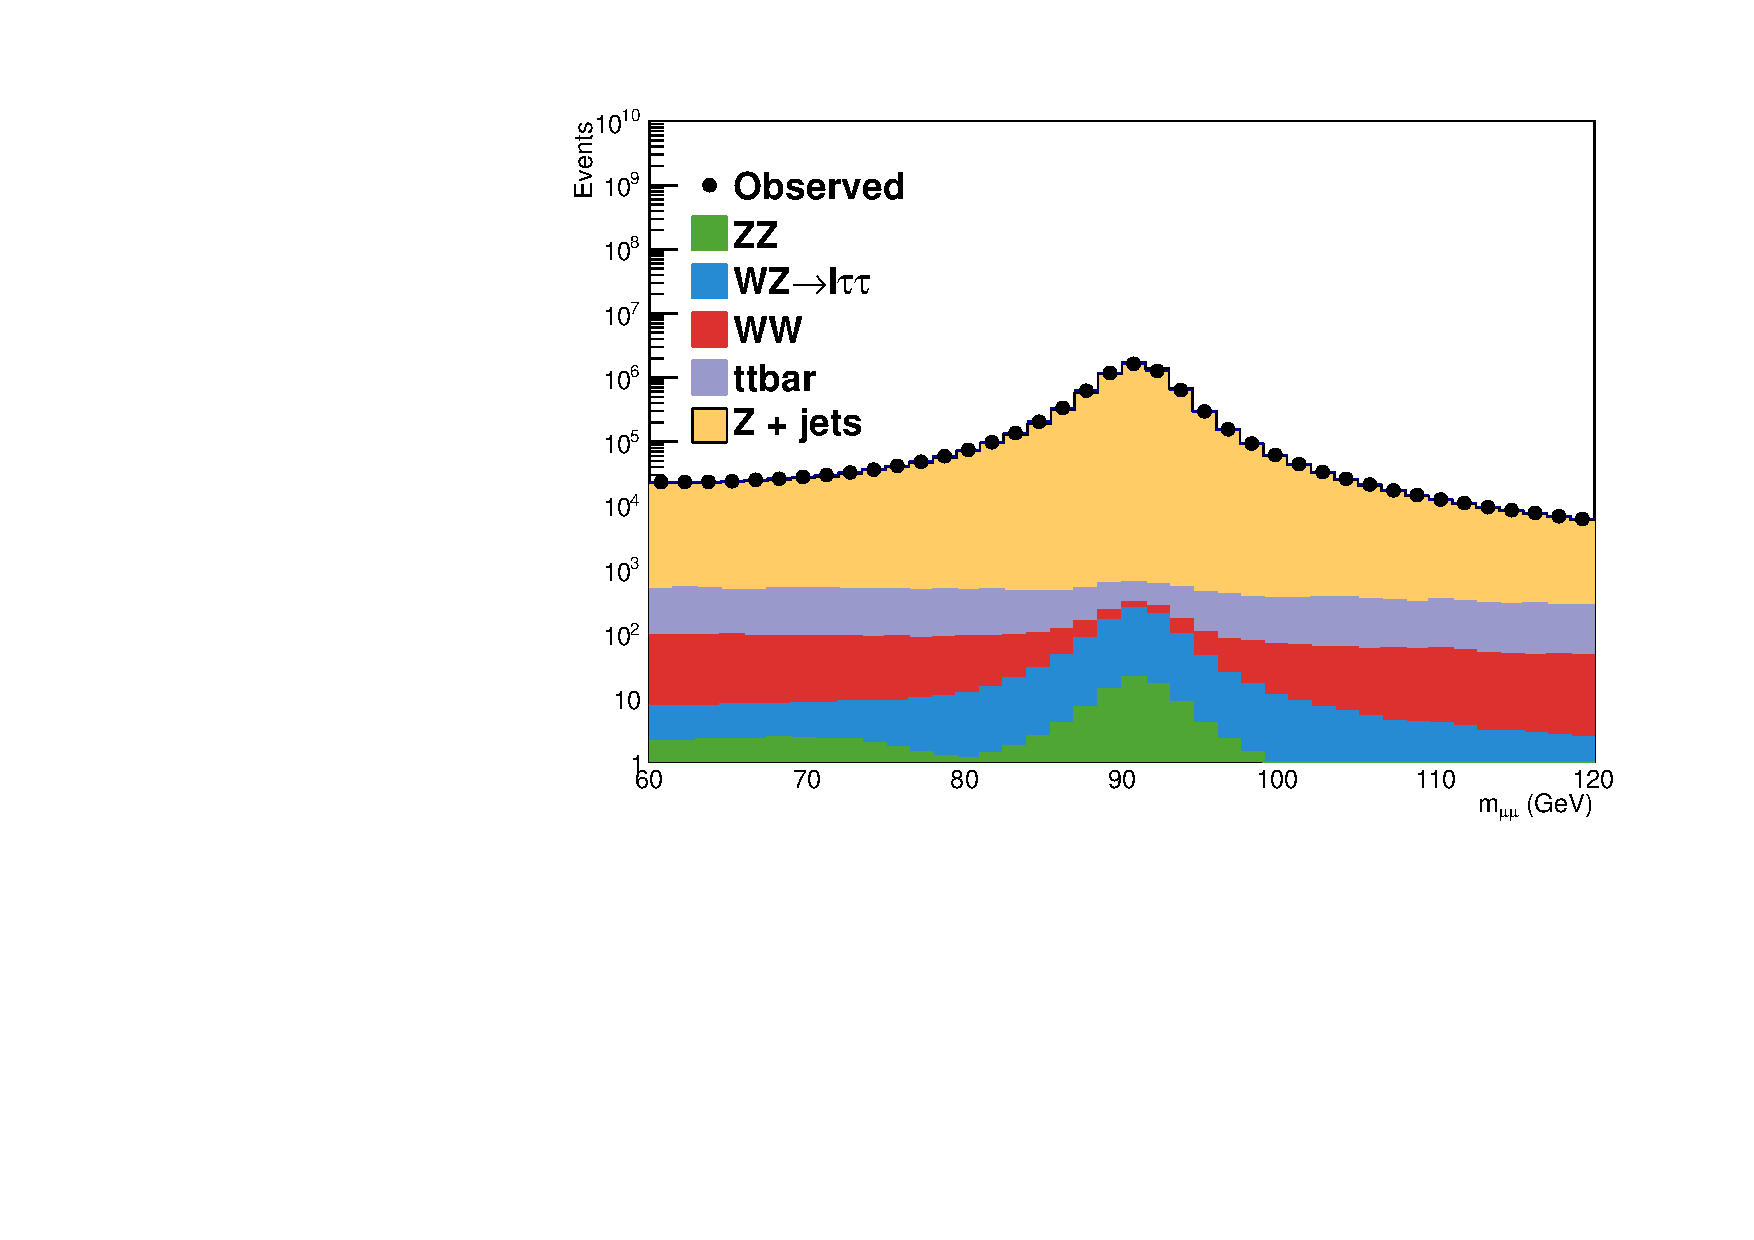
\includegraphics[width=0.49\textwidth]{4_Analisys/pics/8TeV/plots/zmm/mass_rebin_log.pdf}
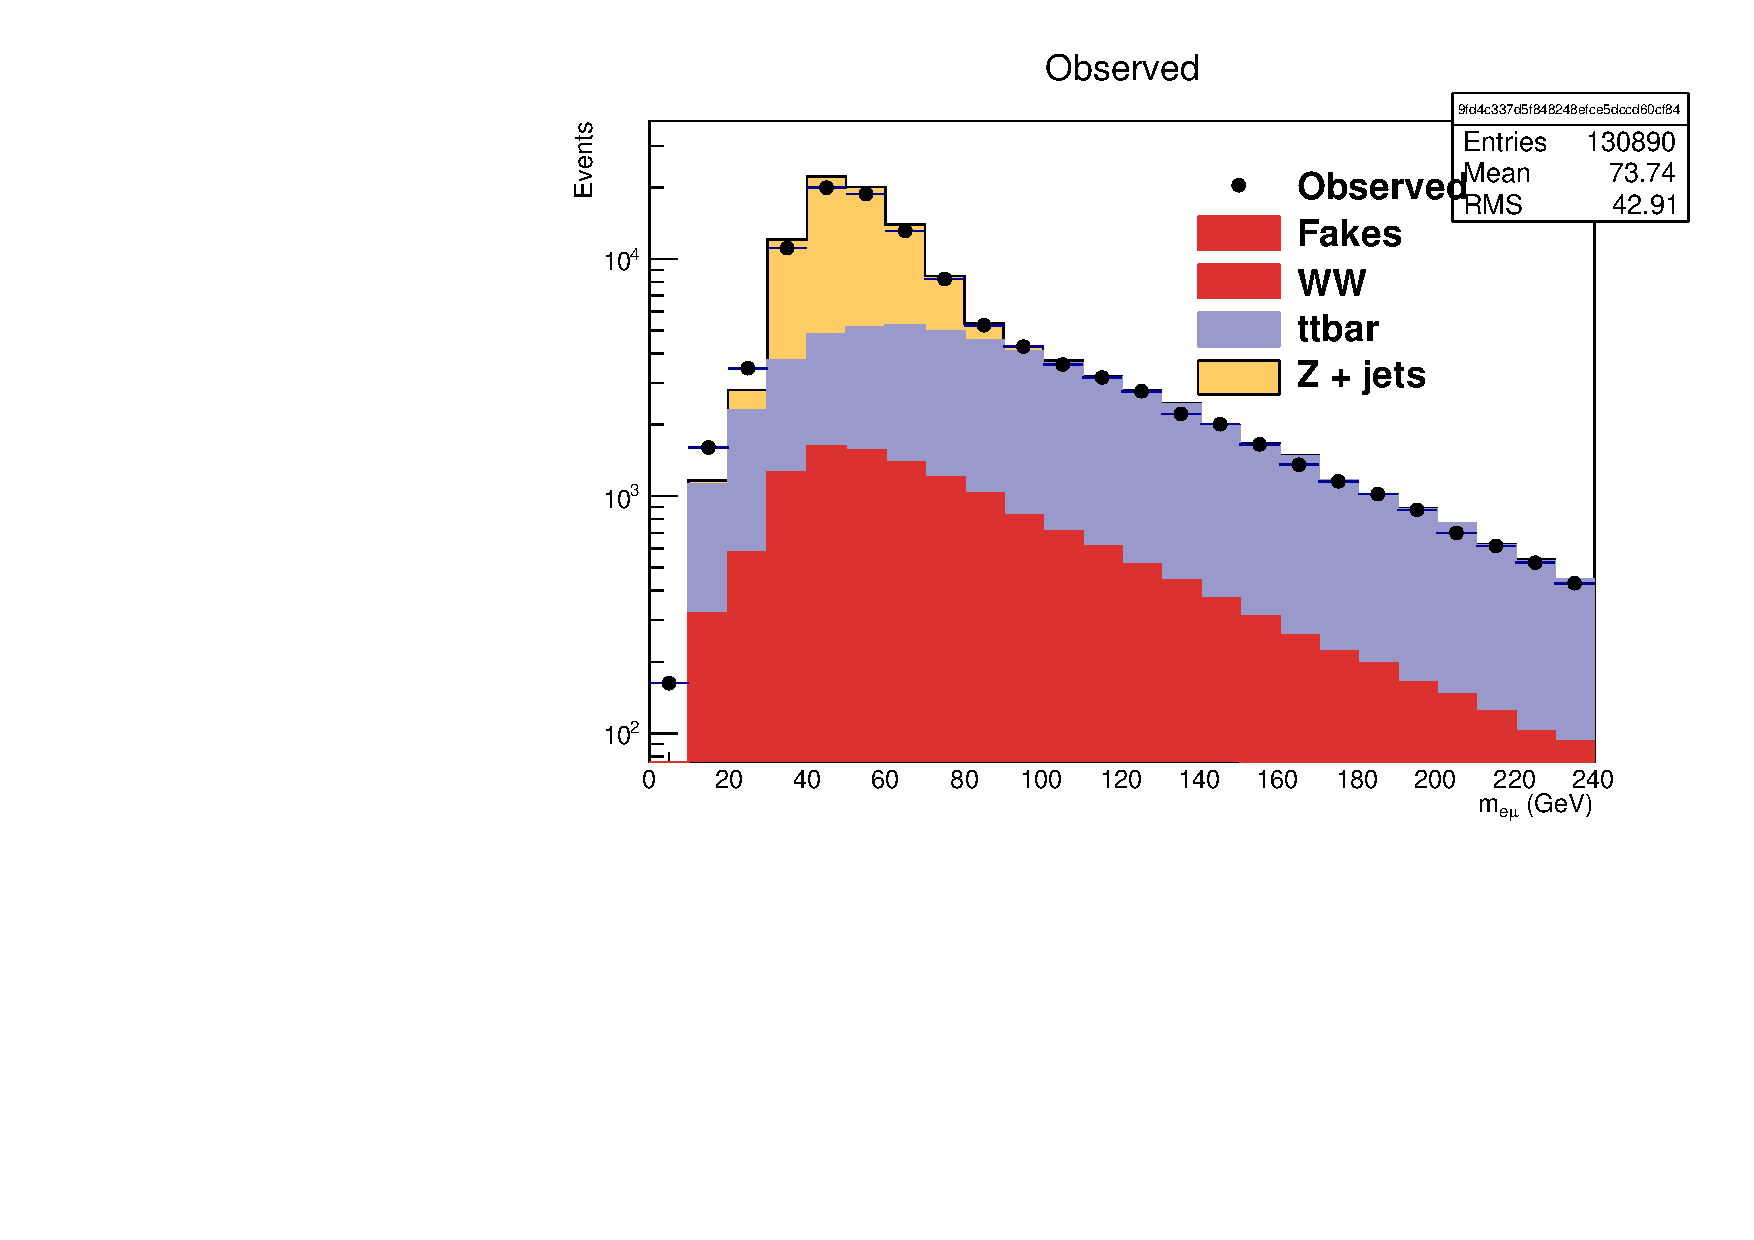
\includegraphics[width=0.49\textwidth]{4_Analisys/pics/8TeV/plots/em/mass_rebin_log-fakes.pdf}\\
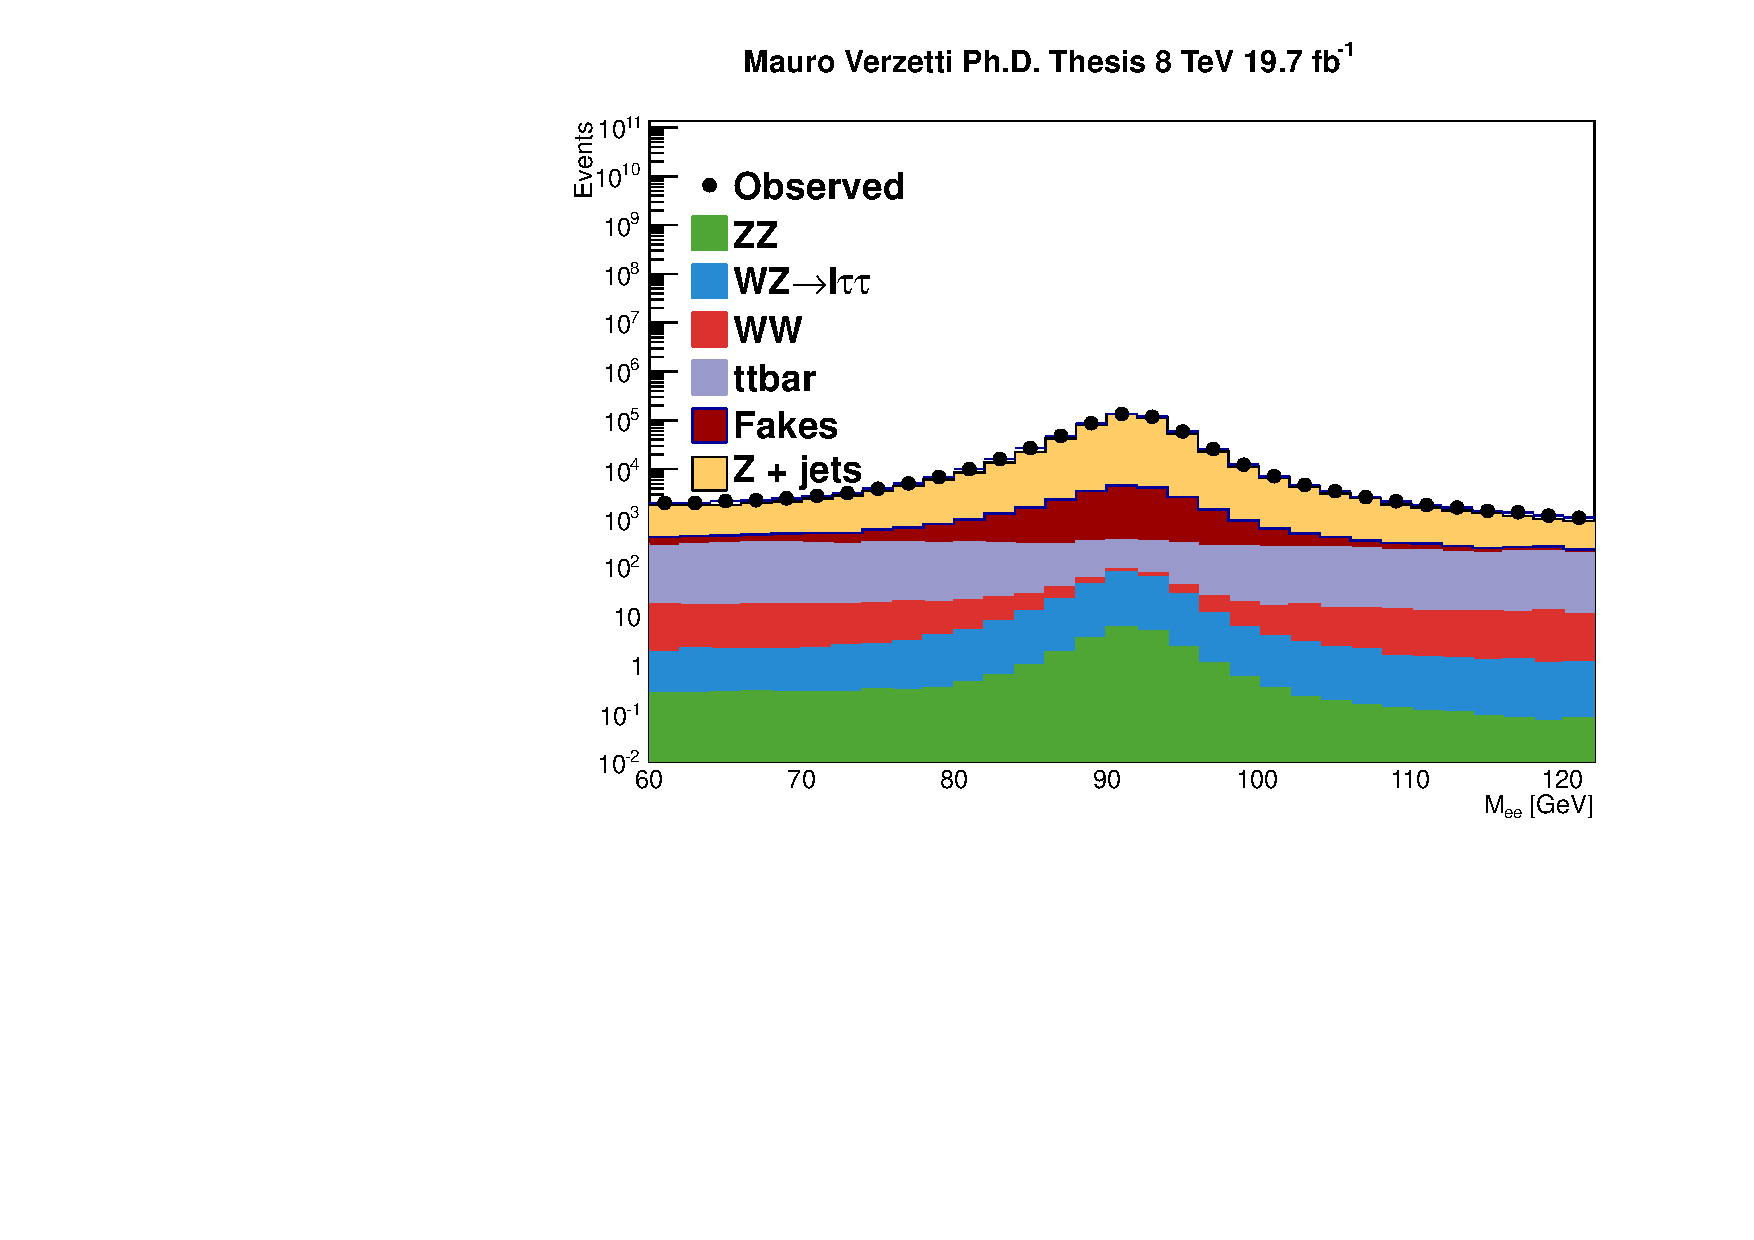
\includegraphics[width=0.49\textwidth]{4_Analisys/pics/8TeV/plots/zee/mass_wfakes_log.pdf}
\caption{Data to MC agreement on 8 TeV data in dedicated $\Z\To\mu\mu$ (top left), $\Z\To \tau\tau \To e\mu$ (top right), and $\Z\To ee$ bottom. The background contributions labeled ``Fakes'' are computed as the reducible background in the main analysis and described in the following section. }
\label{fig:(dis)agreement}
\end{figure}

\subsection{Reducible backgrounds}

The reducible background includes a wide range of processes with quark or gluon jets misidentified as leptons. In these conditions a data-driven background estimation technique is preferred to simulation. Due to these constraints in this work we model the reducible backgrounds with the ``misidentification rate'' (or ``fake rate'') method.

This method consists in defining ``loose'' and ``tight'' selections for the lepton that can be faked by the jets, with the tight selection being the same as the final analysis selection used in this work.
The misidentification probability for a quark or gluon jet satisfying the loose lepton selections to pass the corresponding tight selection can be parametrized by a function $f(\vec{x})$ of a set of kinematic variables, $\vec{x}$, characterizing the event. This probability is measured in a dedicated control region as close as possible, but still disjunct, from the signal region. The misidentification probability is then applied as weight to the events passing all the signal region selections but the tight lepton requirements. These weighted distributions form the background estimation.

We study two possible background estimations: one using the $\rm{jet} \To \ell$ misidentification probability and the other using the $\rm{jet} \To \tau_h$ one. The former method is more inclusive as it accounts for all the sources of reducible backgrounds while the latter ignores those in which an isolated light lepton is mistakenly identified as an hadronic tau candidate. For these processes (i.e. Z+jets, WW, and part of $t\anti{t}$) the latter method relies on MC simulation. 

\subsection{Fake lepton method}
\label{sec:fakemethod}
\subsubsection{Control region definition}
The lepton misidentification probability is measured in a $W$+jets enriched control region.
This region differs from the signal one by requiring the transverse invariant mass of the leading $\ell-\met$ system to be greater than 55 GeV,
and that there are no more than two identified electron or muon candidates in the event. Events containing a well identified hadronic tau are also vetoed removing any overlap with the signal region. In order to mimic the presence of an hadronic tau the event is required to contain an additional jet with \pT above $20$ GeV.

Events falling in the control regions described above are used to train a k-Nearest Neighbor classifier (kNN)~\cite{TMVA}, which allows the parametrization of the misidentification probability in multiple dimensions. All the events entering the control region are used for training purposes.
Each parameter (dimension) is inversely scaled by its variance over the training sample, so that the (scaled) parameters are approximately normally distributed.
Those passing the selection are marked as signal, those failing as background.
To find the misidentification probability at a particular test point in the parameter space, the classifier works searches the $k$ nearest objects to the test point in the training sample.
The predicted efficiency is then the number of signal events in the $k$ neighbors, divided by $k$.
The input variable used for the training are the lepton \pT, the \pT of the jet associated to the lepton, and the number of jets with $\pt > 20$ GeV in the event. 
The first two variables, especially the jet \pT, are found to be strongly correlated to the probability for a jet to be mis-identified as lepton. In particular, the difference of these two variables is linked to the isolation value of the lepton. In the training of the muon misidentification probabilities the logarithm of the jet \pT is used instead of \pT to reduce the steep dependence of the probability with respect to this variable, allowing a larger number of neighbors to be used.
The number of jets was found to improve the description of the background shape. This variable is particularly effective in separating the different processes underlying the reducible background (W, multi-jet, and $t\anti{t}$). Another peculiarity of this variable is that is bound to be $\geq 1$ in the training sample, while it can be zero in the main analysis. The difference is resolved by adding the number of hadronic taus in the event to the number of jets, resulting in a variable with the same range as the training variable.

The contribution of genuine isolated leptons from WZ and ZZ events in the control region is removed using simulated MC events and training dedicated kNN classifiers on them.
The output of the diboson kNN's is then scaled by:

\begin{equation}
\frac{N_{training}^{MC}}{N_{training}^{data}}\frac{\mathcal{L}^{data}}{\mathcal{L}_{eff}^{MC}}
\end{equation}

where $N_{training}^{i}$ is the number of events used for training of data or MC and $\mathcal{L}^{i}$ the recorded or equivalent lminosity. The output of the diboson kNN is finally subtracted to the output of the kNN trained on data.\footnote{Another equivalent option would have been to directly inject the simulated events in the training sample with negative weight proportional to the luminosity difference, but this method has been found to yield inconsistent results, most likely due to a wrong implementation in the TMVA framework.}

\subsubsection{kNN optimization and systematic uncertainties}
\label{sec:kNN_uncertainties}

The only adjustable parameter in the kNN training is the number of neighbors used to extract the probability. The optimal neighbors number is function of both the dependency of the probability to the different observables (more or less steeply varying) and of the statistics of the training sample. A large number of neighbors yields a very accurate results, at the price of a reduced ability to describe abrupt changes in the probability function.

It is therefore important to define a procedure to infer the optimal number of neighbors for each sample and the working point used in the final analysis. This evaluation is performed with a bootstrapping technique.
Each training sample is initially split in two uneven sub--samples, one containing 90\% of the events and the other the remaining 10\%. In order to remove any bias due to the run period (different pileup conditions) the lesser dataset is evenly sampled from the full dataset. This procedure is repeated ten times to obtain a set of mutually exclusive pairs of ``large'' and ``small'' samples. Subsequently, a training of the kNN classifier is performed on each large sample and applied to the small one. This procedure ensure a total decoupling between testing and training samples. The small size difference between the large sample and the full dataset also ensures that the results inferred from the major dataset are still statistically valid for the full one. The outcome of the ten training and testing cycles is then combined. 

The full process is repeated scanning a wide range of possible neighbors values. A strong limiting factor for this method is the significant computing resource usage, as the computing complexity of training and testing of the classifier is proportional to the number of neighbors used. The choice of the tested points and their maximum value are a direct consequence of this limitation: as the number of neighbors increases, the scan becomes more coarse.

For each tested neighbor working point, the shape of important physics observables is computed from the weighted sum of all the events in the small samples and from the passing events. The two shapes are compared using as figure of merit the $\chi^2$ between the two shapes. The physical observable used for the $\chi^2$ minimization is the scalar sum of the \pT of the two leptons and the jet, similar to the $L_T$ variable used further on in the analysis. Other variables were also considered and found to yield compatible results. 

The minimum of the scan is taken as reference value of number of neighbors to be used for training in the analysis. A parabolic fit around the minimum is performed to estimate the one sigma confidence interval as the value for which the parabolic fit is $fcn(i) = \chi^2_{min} + 1$. This confidence interval reflects both the statistical uncertainties on the training sample and the related uncertainty on the choice of the parameters. For each channel and each lepton, three classifiers are trained with the corresponding central values and one sigma boundaries.

A summary of the chosen minima and confidence interval boundaries is available in Table \ref{tab:kNN_minima}. A graphic representation of a sample scan is shown in Fig. \ref{fig:kNN_minima_sample}. The misidentification rate observed in the training sample is displayed in Fig. \ref{fig:fake_rate_sample} overlaid with the output of the respective kNN classifier.


\begin{table}

\caption{Minimization points for each kNN scan and relative uncertainties as obtained from a parabolic fit}

\centering
\begin{tabular}{|c|c|c|c|c|}
\hline
channel & lepton & $-1\,\sigma$ & central value & $1\,\sigma$ \\
\hline
\multicolumn{5}{|c|}{7 TeV} \\
\hline
\multirow{2}{*}{ $\mu\mu\tau_h$ }& leading muon & 15 & 20 & 60\\
& sub-leading muon & 11 & 20 & 49\\
\hline
\multirow{2}{*}{ $e\mu\tau_h$ }& muon & 7 & 20 & 30\\
& electron & 634 & 1000 & 1807\\
\hline
\multirow{2}{*}{ $ee\tau_h$ }& leading electron & 35 & 200 & 686\\
& sub-leading electron & 381 & 1200 & 1723\\
\hline
\multicolumn{5}{|c|}{8 TeV} \\
\hline
\multirow{2}{*}{ $\mu\mu\tau_h$ }& leading muon & 28 & 40 & 73\\
& sub-leading muon & 30 & 40 & 63\\
\hline
\multirow{2}{*}{ $e\mu\tau_h$ }& muon & 16 & 20 & 30\\
& electron & 664 & 1400 & 2136\\
\hline
\multirow{2}{*}{ $ee\tau_h$ }& leading electron & 218 & 400 & 552\\
& sub-leading electron & 605 & 1000 & 2201\\
\hline
\end{tabular}

\label{tab:kNN_minima}
\end{table}

\begin{figure}
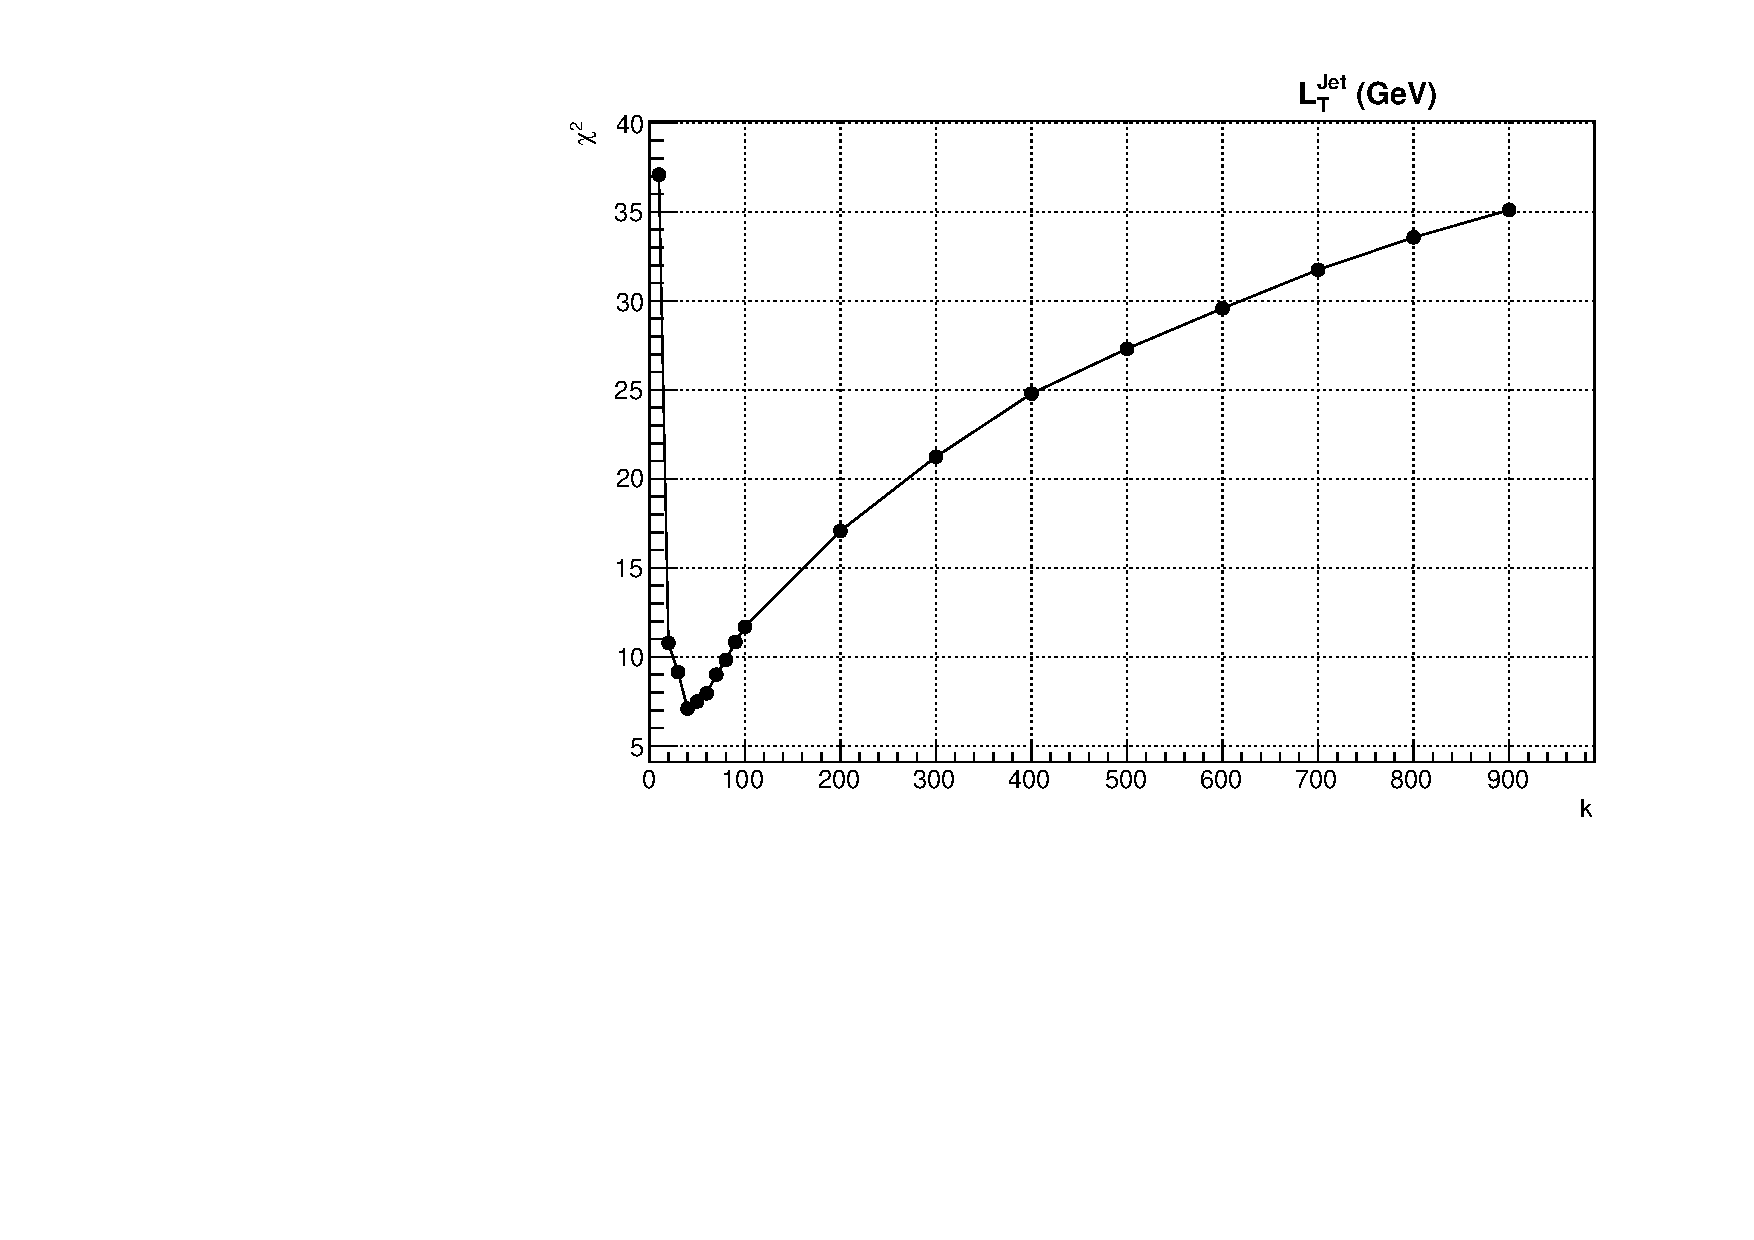
\includegraphics[width=0.5\textwidth]{4_Analisys/pics/8TeV/ProfileNeighbors/MM/h2taucuts020/LT_chi2.pdf}
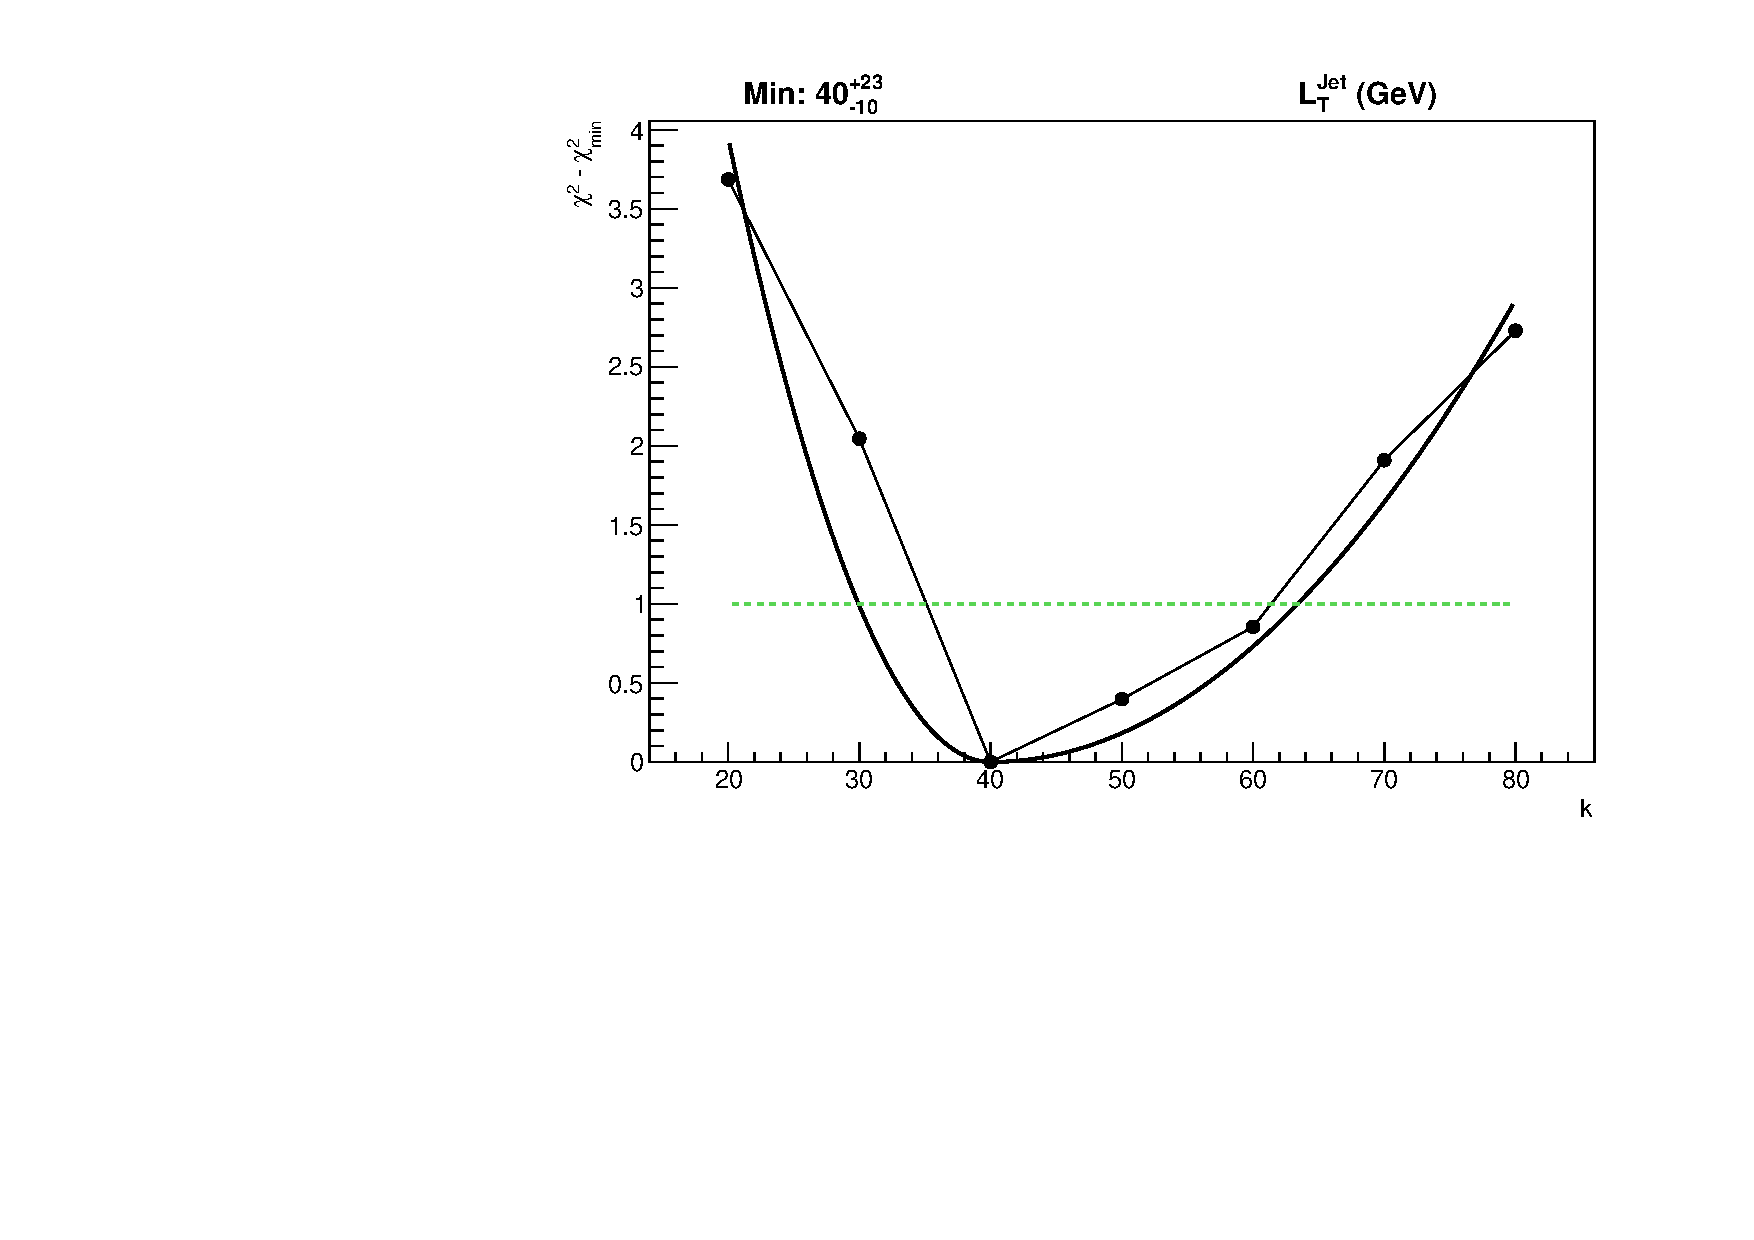
\includegraphics[width=0.5\textwidth]{4_Analisys/pics/8TeV/ProfileNeighbors/MM/h2taucuts020_LT.pdf} \\
\caption{\chisq scan of different neighbors value (left) and corresponding minima fit (right) for sub-leading muons in the $\mu\mu\tau_h$ channel. The variable used for the scan is the scalar sum of the \pT of the two leptons and the jet}
\label{fig:kNN_minima_sample}
\end{figure}

\begin{figure}
\centering
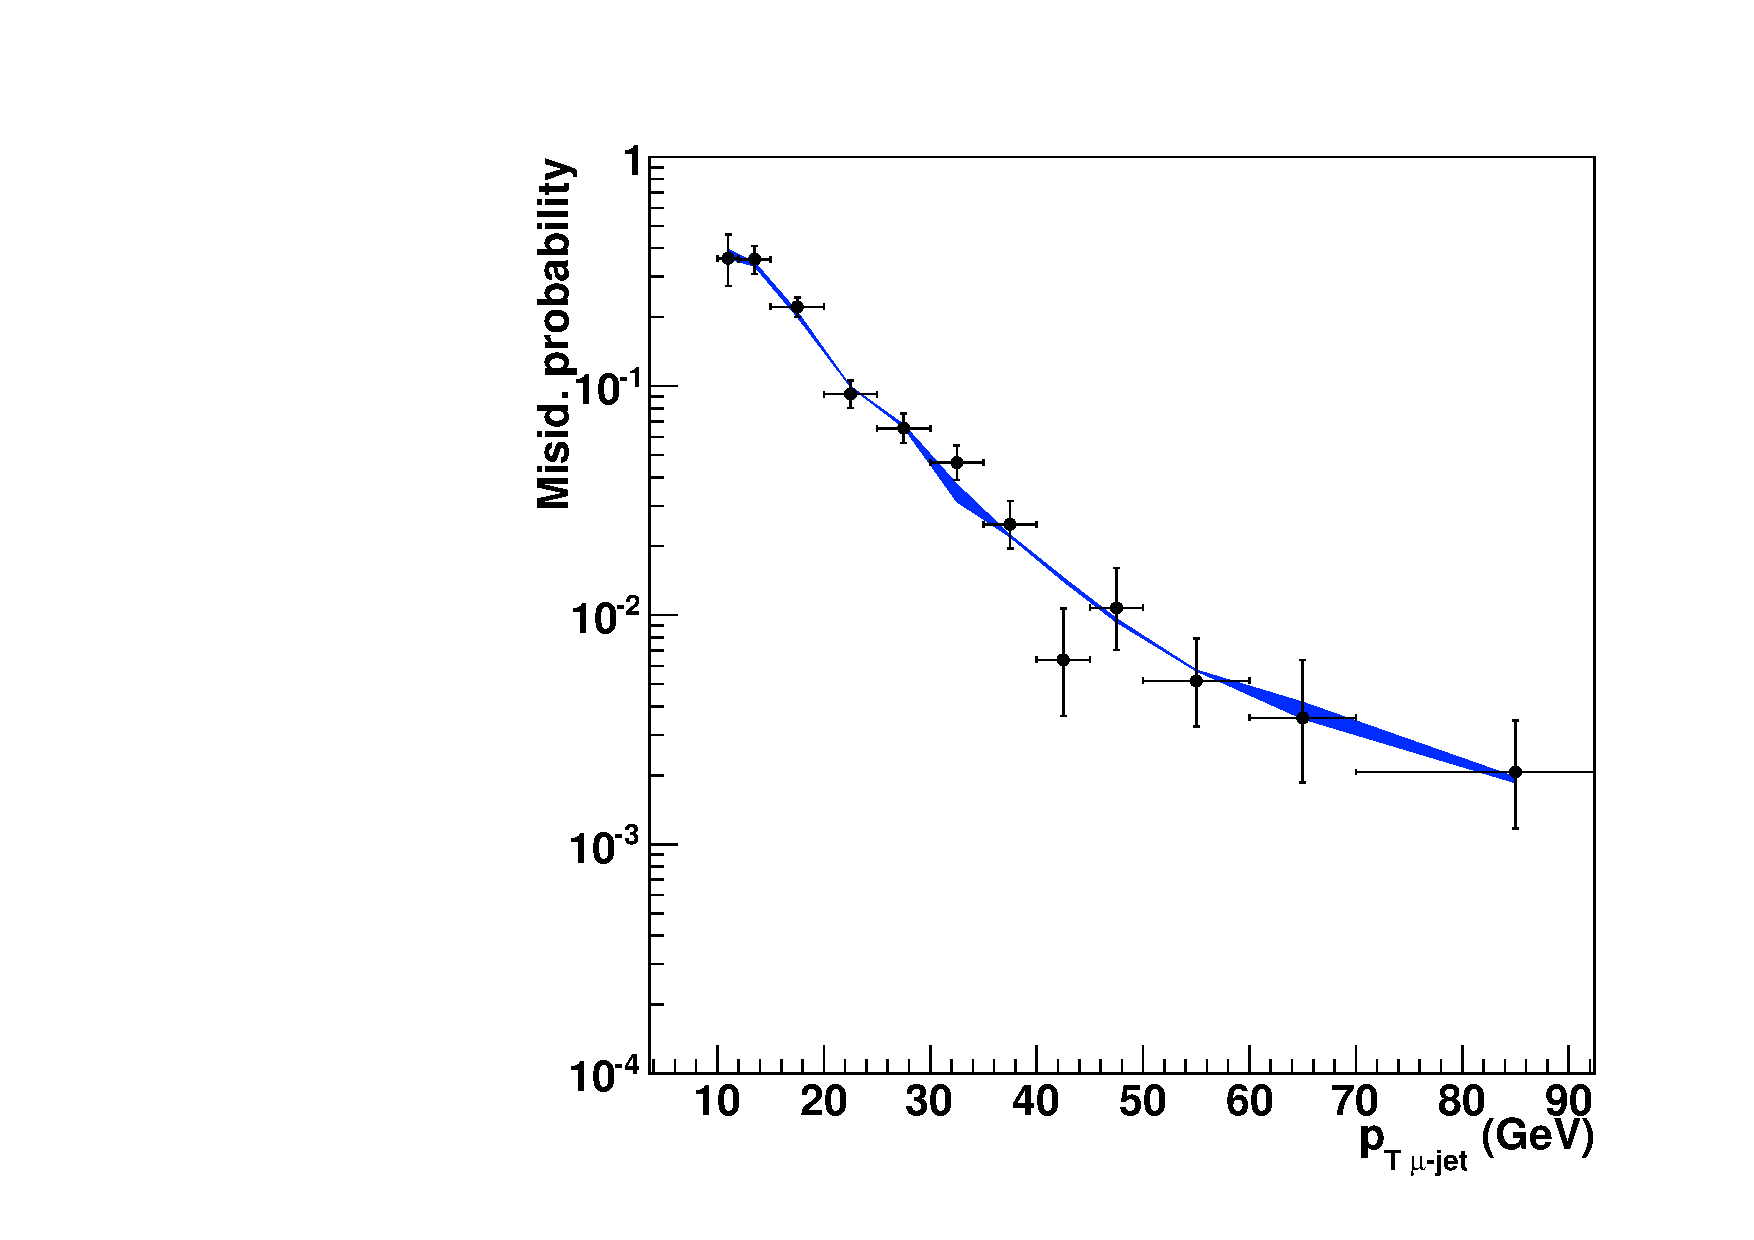
\includegraphics[width=0.49\textwidth]{4_Analisys/pics/8TeV/plots/fakerates/m_mmt_subleading_kNN_muonJetPt.pdf}
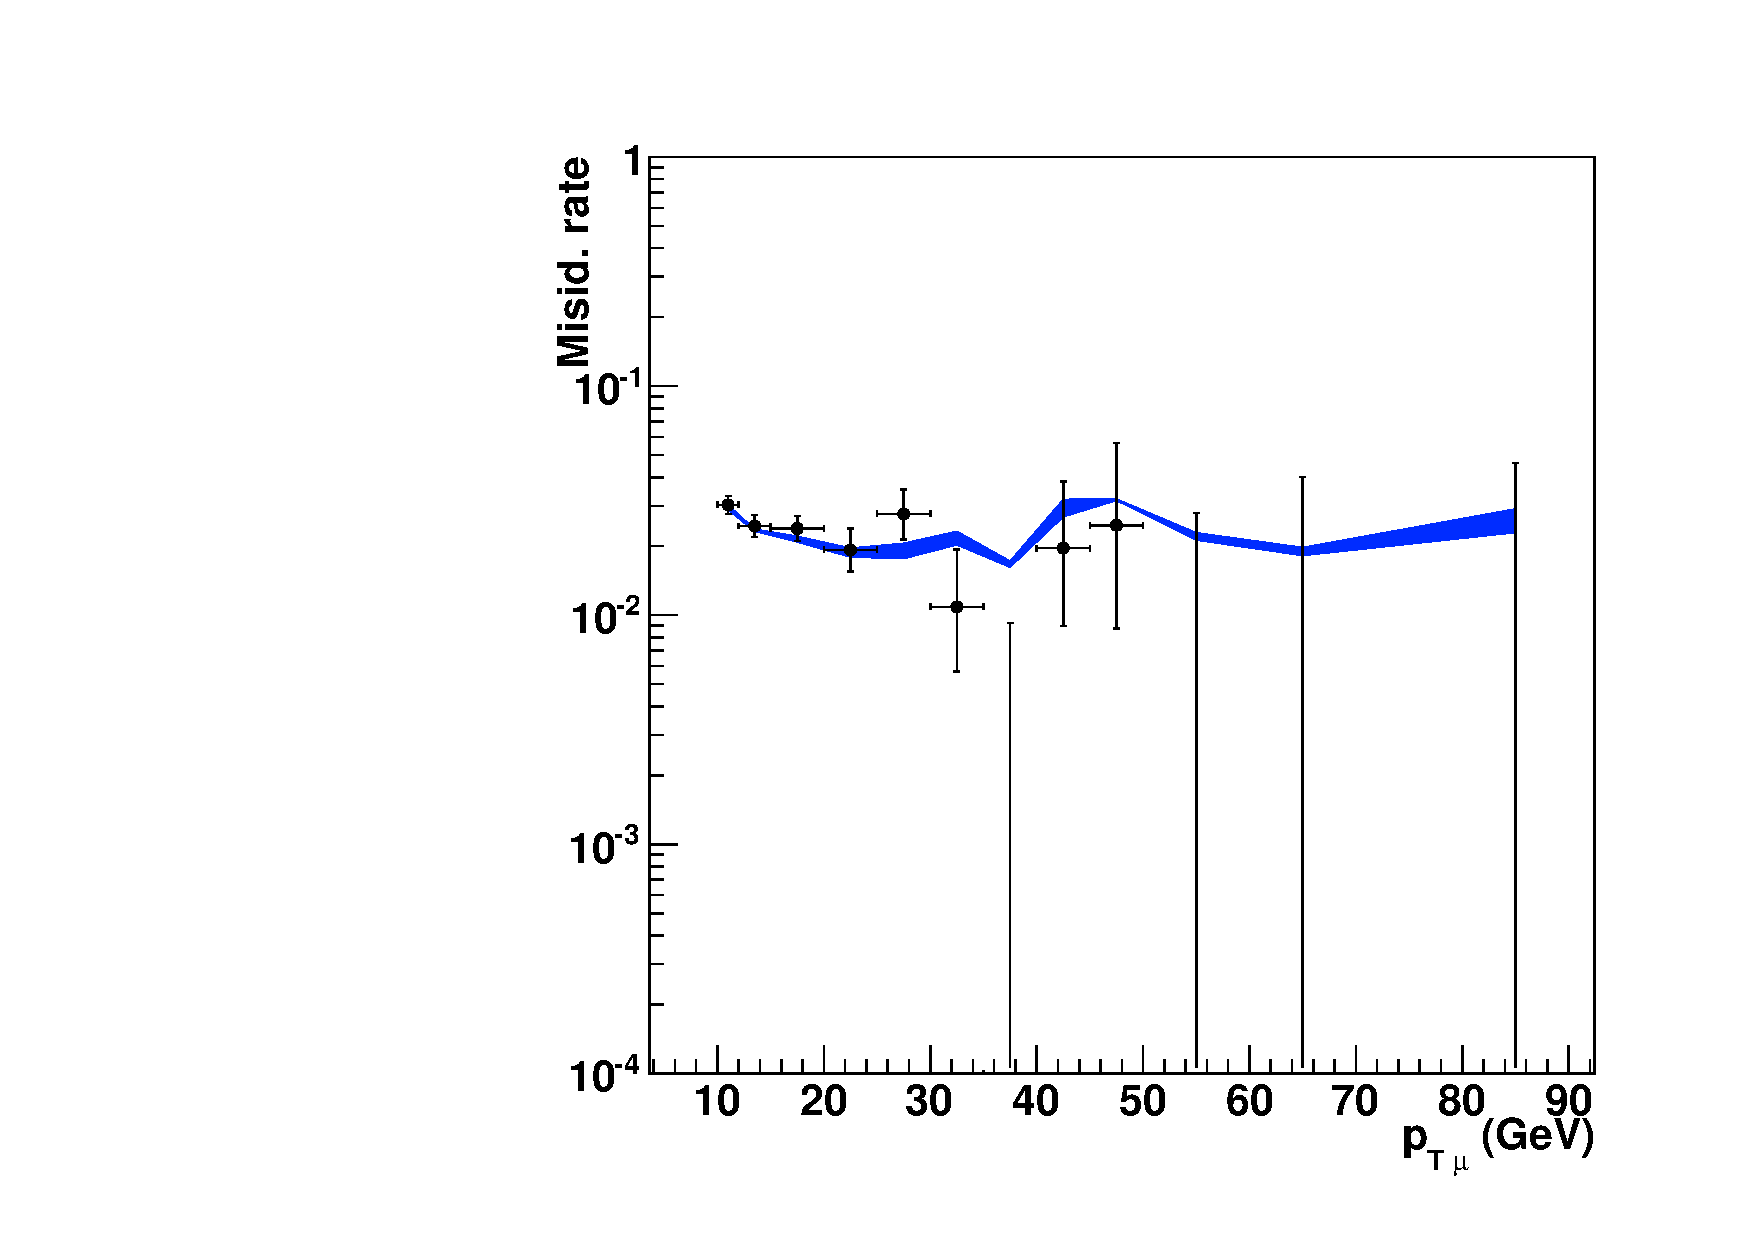
\includegraphics[width=0.49\textwidth]{4_Analisys/pics/8TeV/plots/fakerates/m_mmt_subleading_kNN_muonPt.pdf}\\
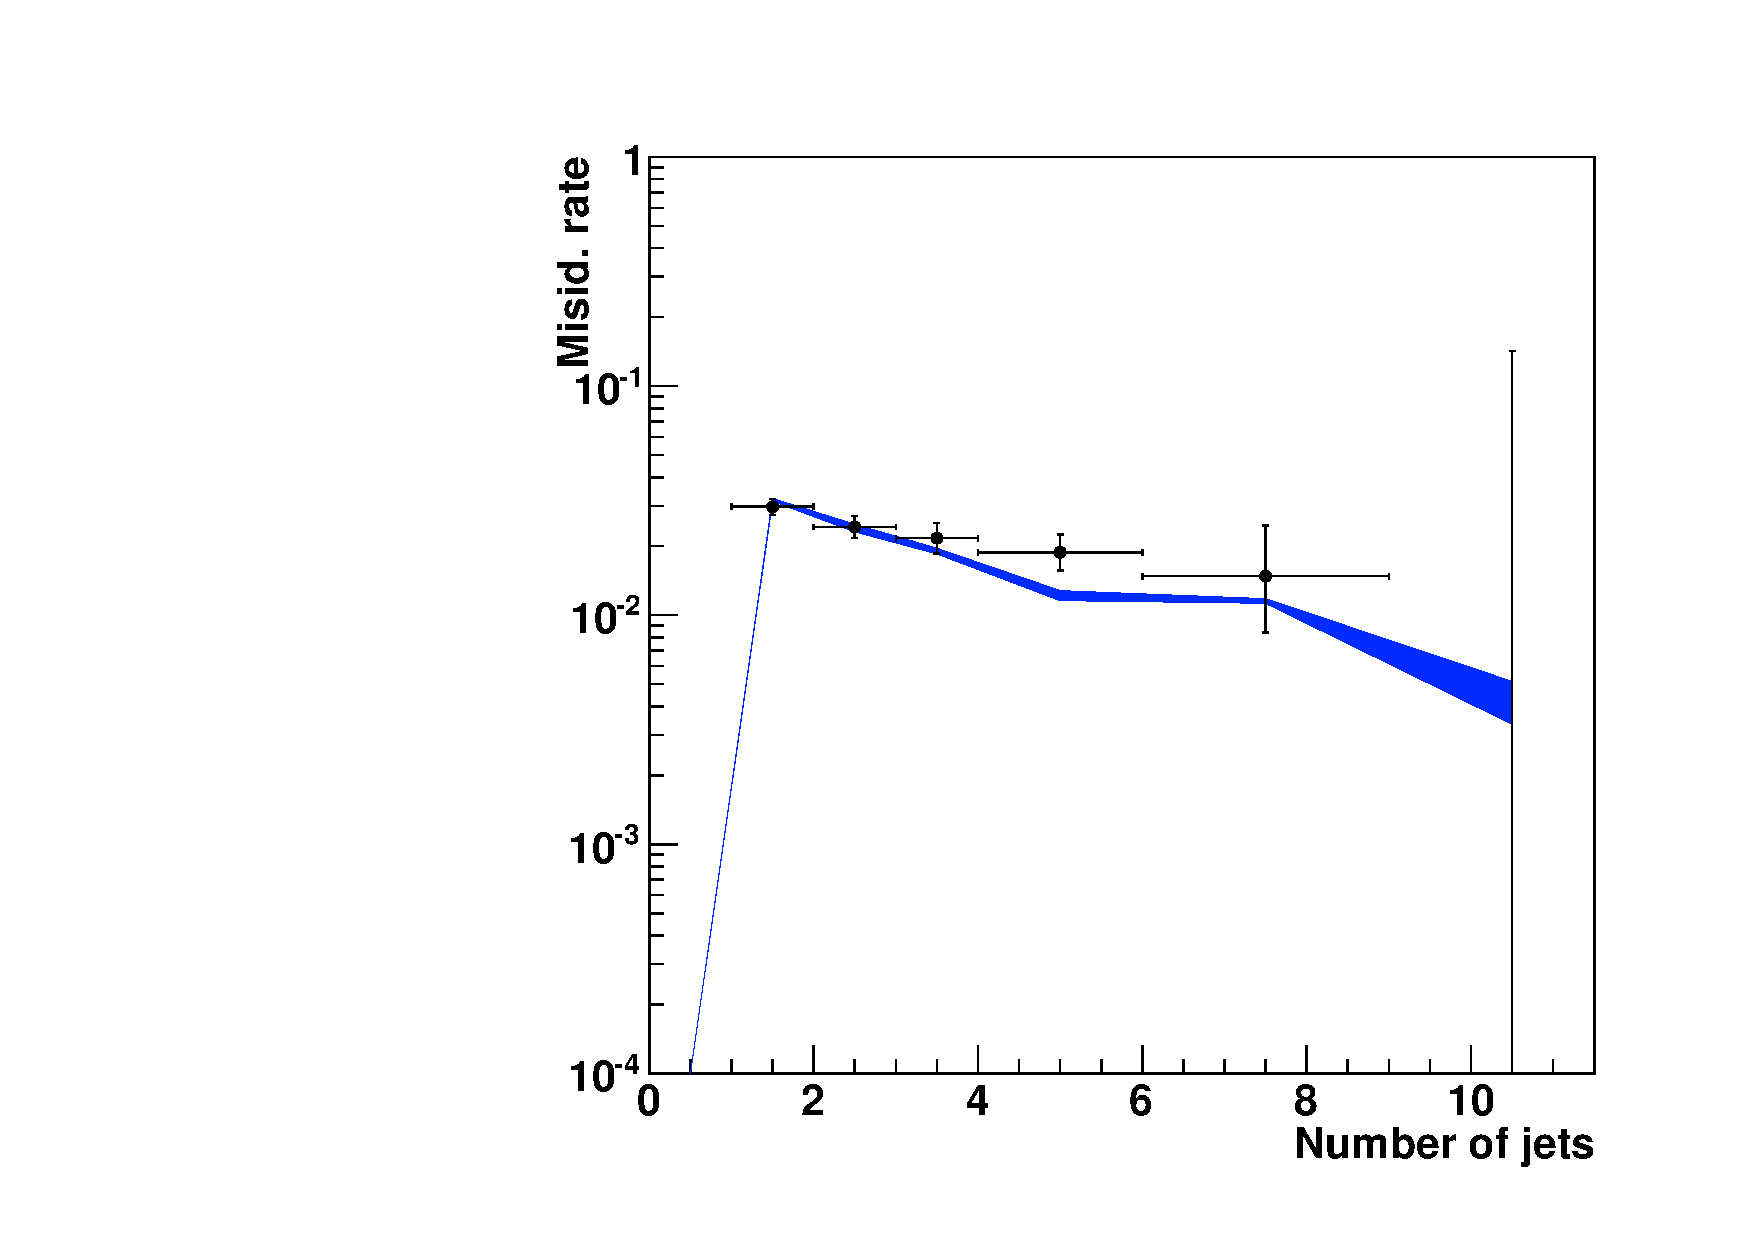
\includegraphics[width=0.49\textwidth]{4_Analisys/pics/8TeV/plots/fakerates/m_mmt_subleading_kNN_numJets20.pdf}
\caption{Measured misidentification for sub-leading muons in the $\mu\mu\tau_h$ dedicated training sample. The blue band represents the output of the kNN estimation and its related uncertainty.}
\label{fig:fake_rate_sample}
\end{figure}


\subsubsection{Background shape extraction}
The contribution to the signal region from backgrounds containing a given fake object is estimated using a ``anti-isolated'' sideband in which the loose, but \emph{not} the tight, 
selection requirement is satisfied for that object. Events can therefore be divided into three categories:

\begin{enumerate}
\item Events in which the first lepton fails the tight requirements are weighted by $w_1(\vec{x}) = f_1(\vec{x})/(1-f_1(\vec{x}))$
\item Events in which the second lepton fails the tight requirements are weighted by $w_2(\vec{x}) = f_2(\vec{x})/(1-f_2(\vec{x}))$
\item Events in which the both lepton fail the tight requirements are weighted by $w_1(\vec{x}) \cdot w_2(\vec{x})$
\end{enumerate}

Each weighted category represents the contribution in the signal region of the background components with jets being identified as one or both the light leptons. As the events where jets are mis-reconstructed as both leptons are included in both the category 1 and 2, it is necessary to remove the double-counting by subtracting the weighted events of category three, obtaining:

\begin{equation}
N_{bkg} = N_1 + N_2 - N_3
\end{equation}

where $N_{bkg}$ is the number of background events and $N_i$ is the scaled number events in category $i$.

%Sys uncertainty
Uncertainties on the kNN training, evaluated as described above, are propagated to the background estimation by computing event weights with classifiers trained with the central value and the two one--sigma boundaries. The differences between them are taken as systematic uncertainty.

%Empty bins
In rare cases, especially in the tail of the kinematic distributions, statistical fluctuations cause the number of weighted events in category three to exceed the sum of the other two categories, and therefore the expected yield in that bin becomes negative. In these cases the yield for that bin is set to the value of category three only, relying on the much larger statistics present in that sideband.


%

\subsection{Validation of the fake lepton method}

The reducible background estimation is validated in two ``fake tau'' control regions which are dominated by fake $\tau_h$ candidates.
This exercises all mechanisms of the reducible background estimation, since the $\tau_h$ candidate never participates in the misidentification rate method.
The light-lepton same-charge requirement is maintained, but the isolation requirement of the $\tau_h$ candidate is inverted and in one of the regions the charge of the tau is required to be the same as the leptons.
This regions are dominated by W+jets and $t\anti{t}$ backgrounds.
Comparison between measured and simulated kinematic distributions in these control regions is shown for the $\mu\mu\tau_h$, $e\mu\tau_h$ and $ee\tau_h$ channels in Figs.~\ref{fig:LLT_mmt_f3_control_7TeV}--\ref{fig:LLT_eet_f3_control_8TeV} respectively.
Reasonable agreement is observed between the measured and predicted backgrounds.

\begin{figure}
\begin{center}
  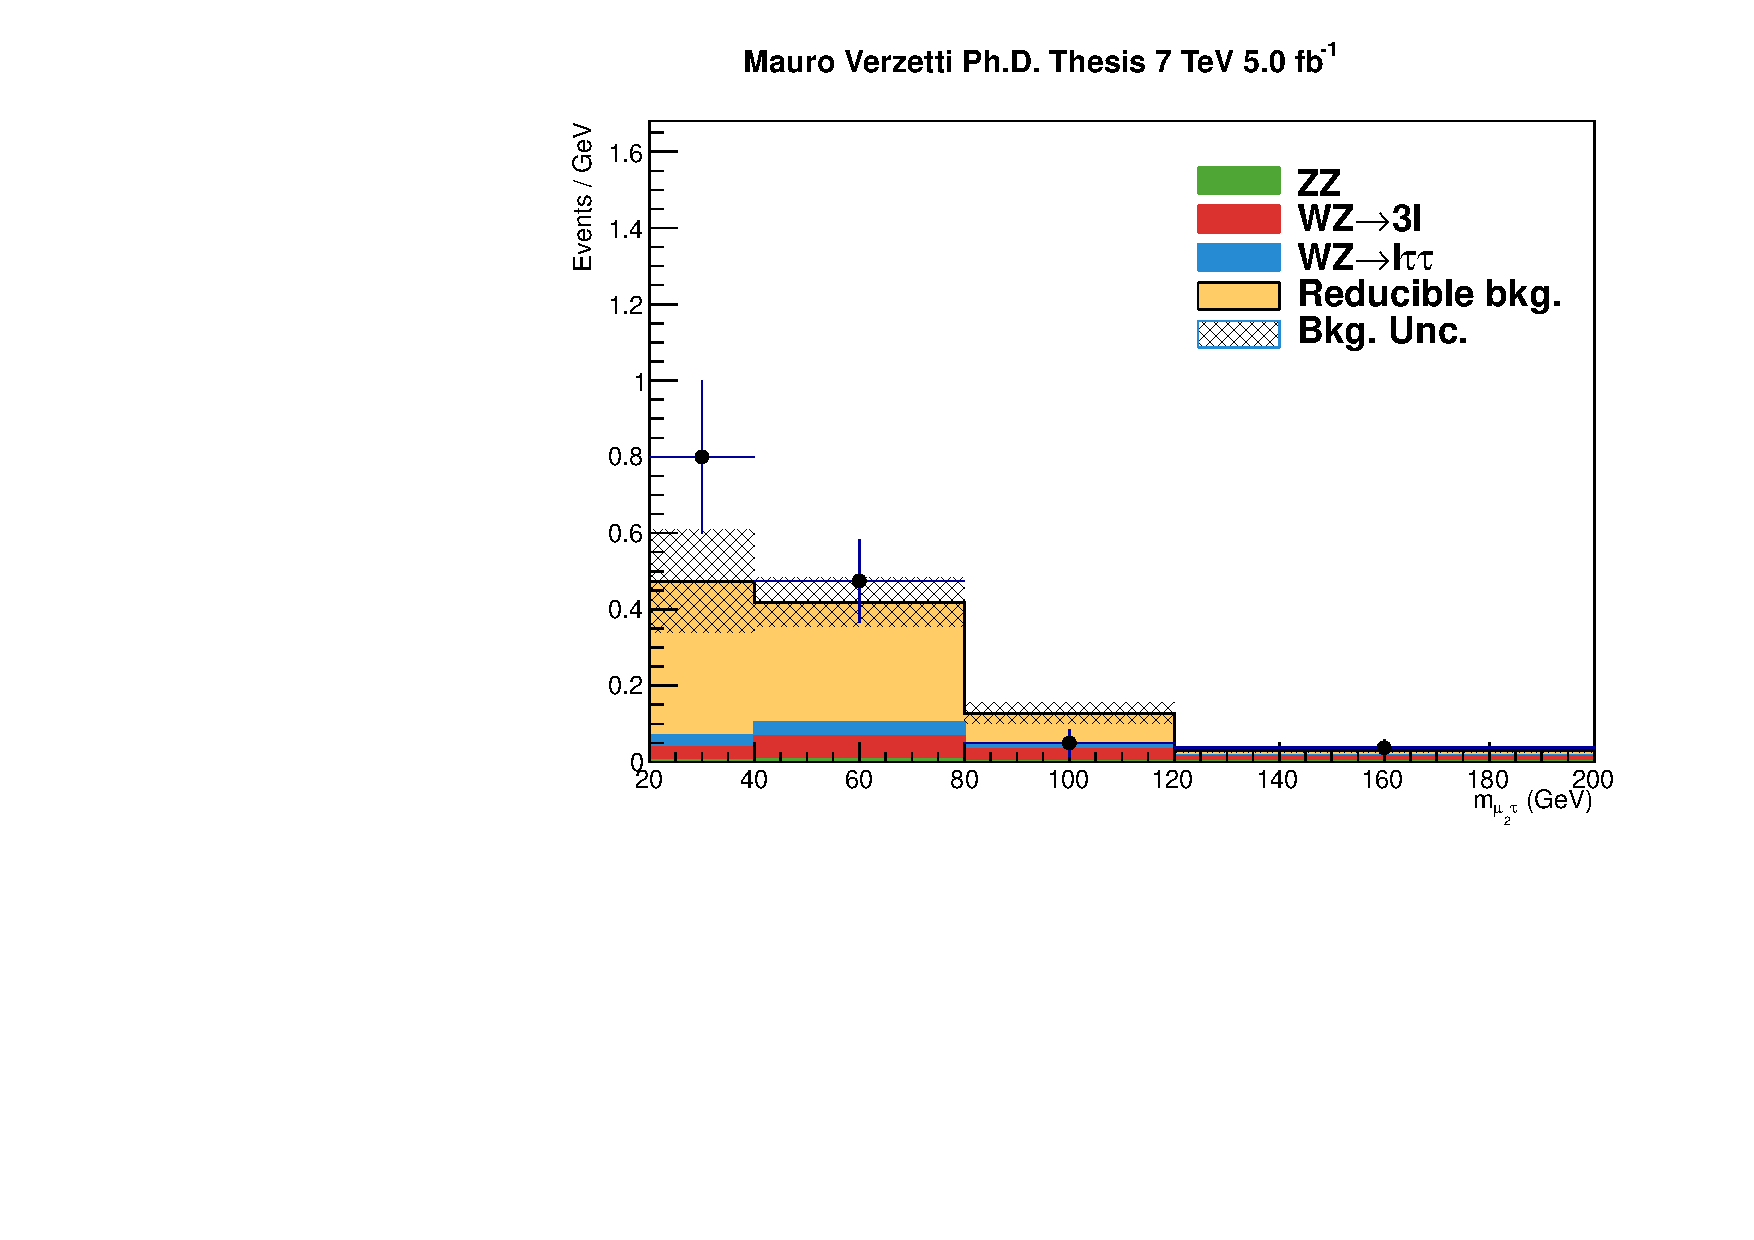
\includegraphics[width=0.49\textwidth]{4_Analisys/pics/7TeV/plots/mmt/f3/Full/final-f3-subMass-Full.pdf}
  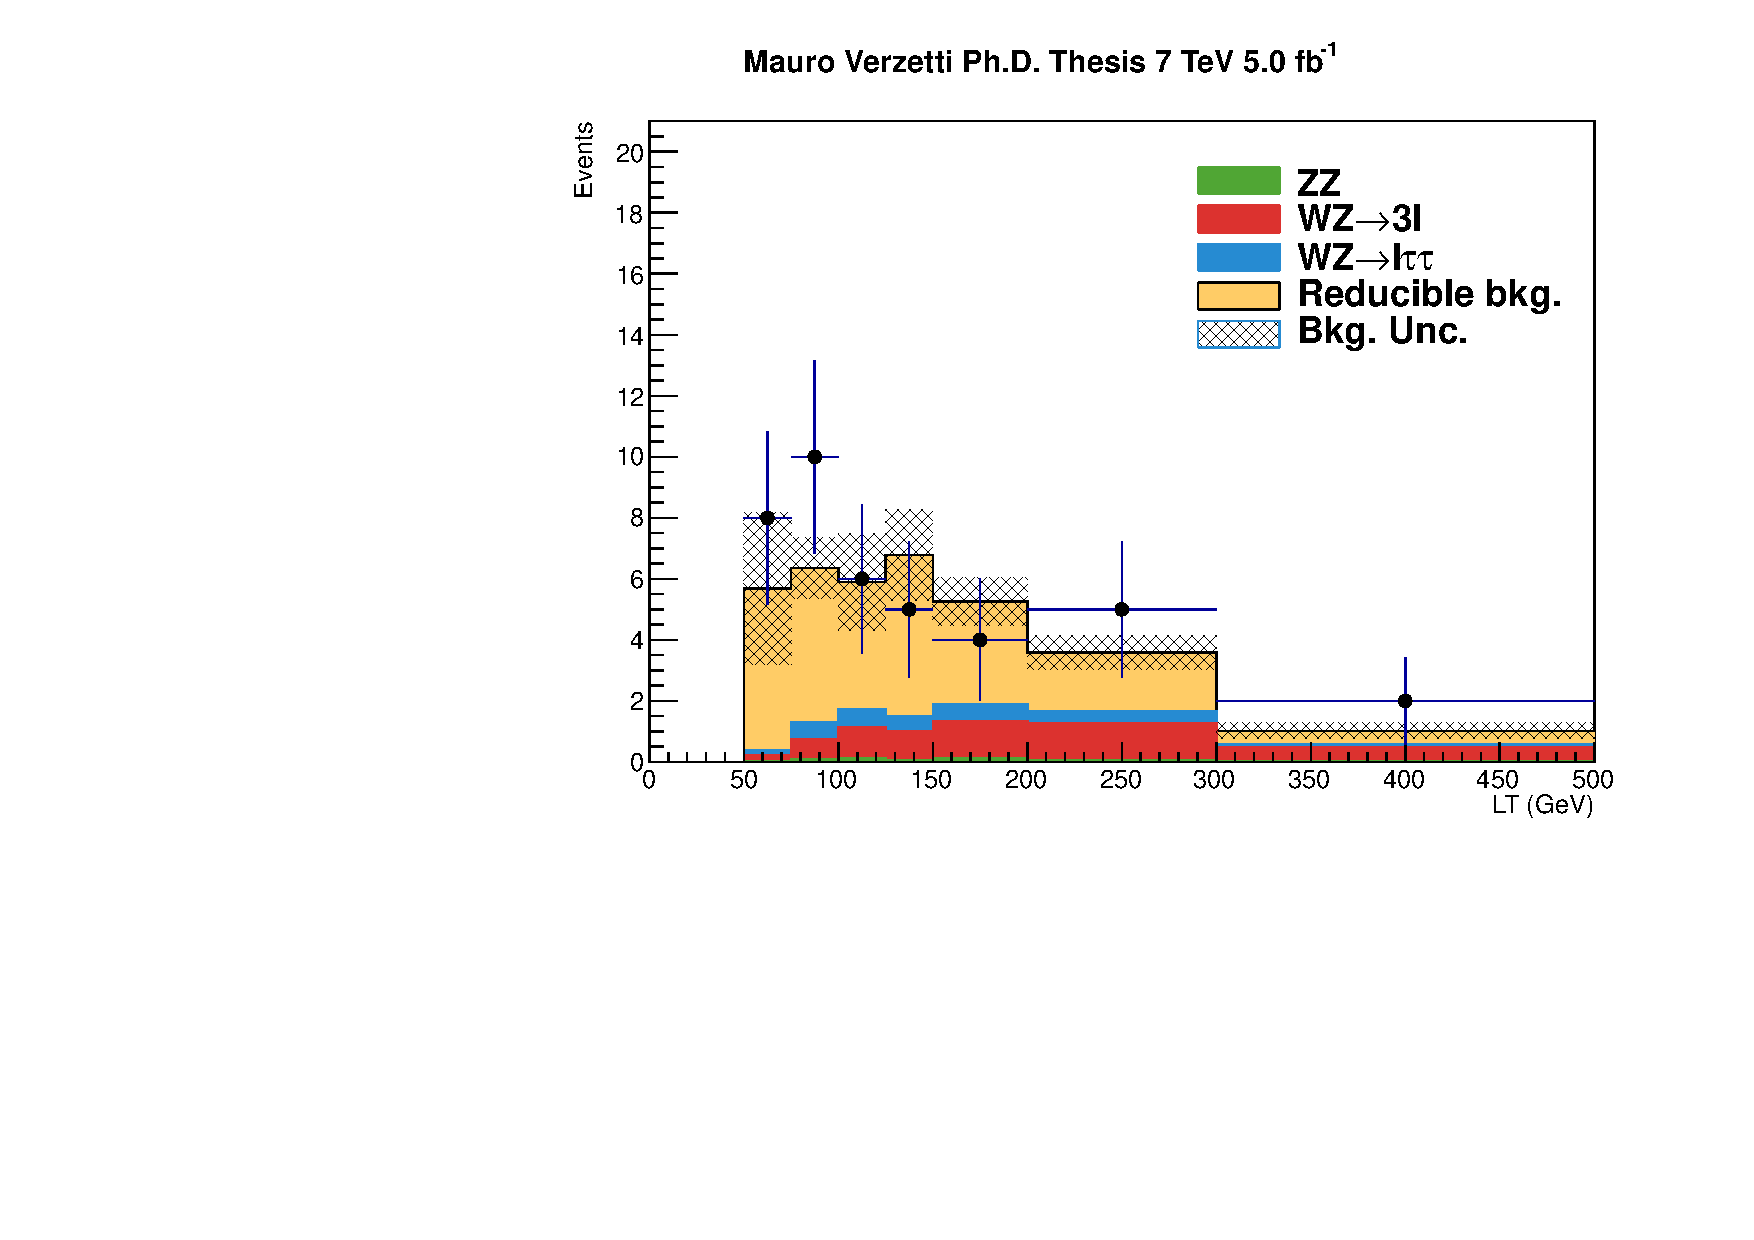
\includegraphics[width=0.49\textwidth]{4_Analisys/pics/7TeV/plots/mmt/f3/final-LT.pdf}\\
  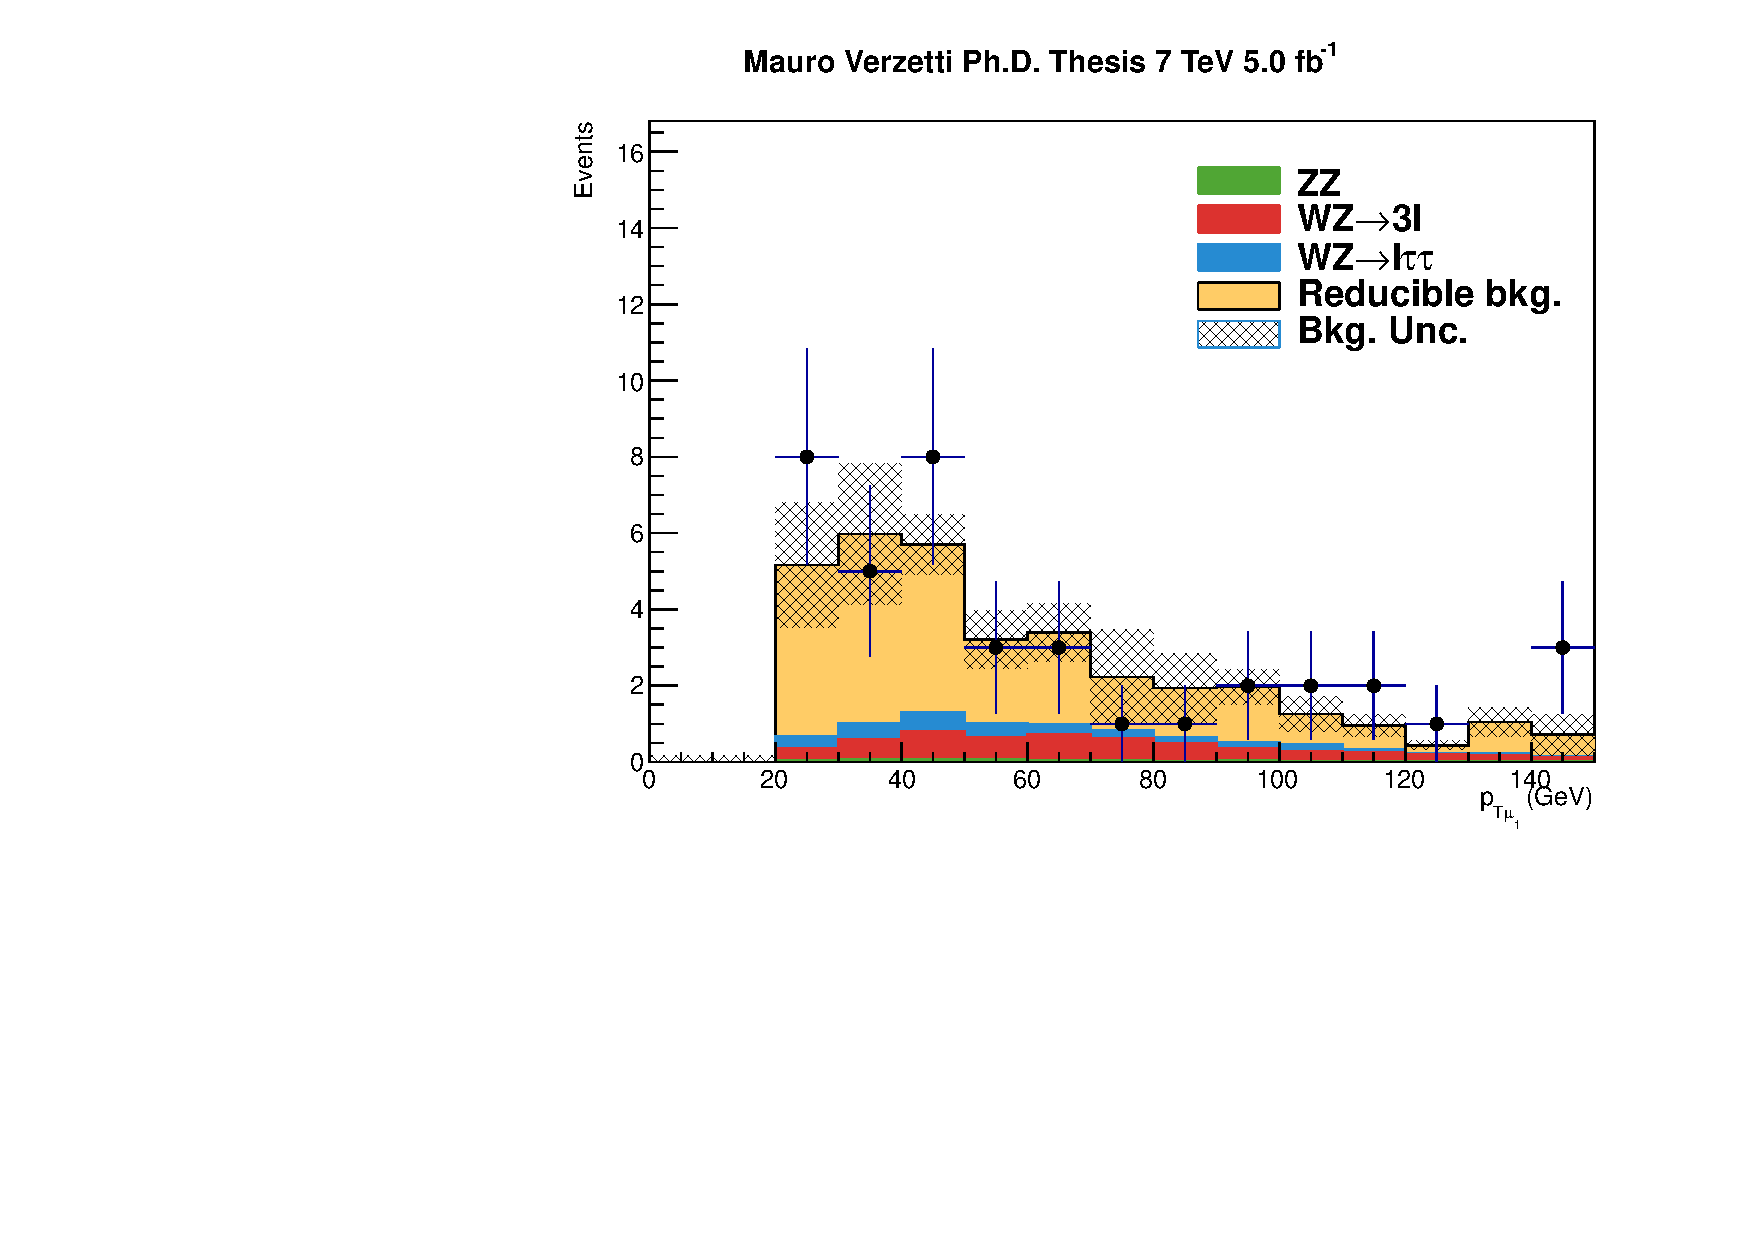
\includegraphics[width=0.49\textwidth]{4_Analisys/pics/7TeV/plots/mmt/f3/Full/final-f3-m1Pt-Full.pdf}
  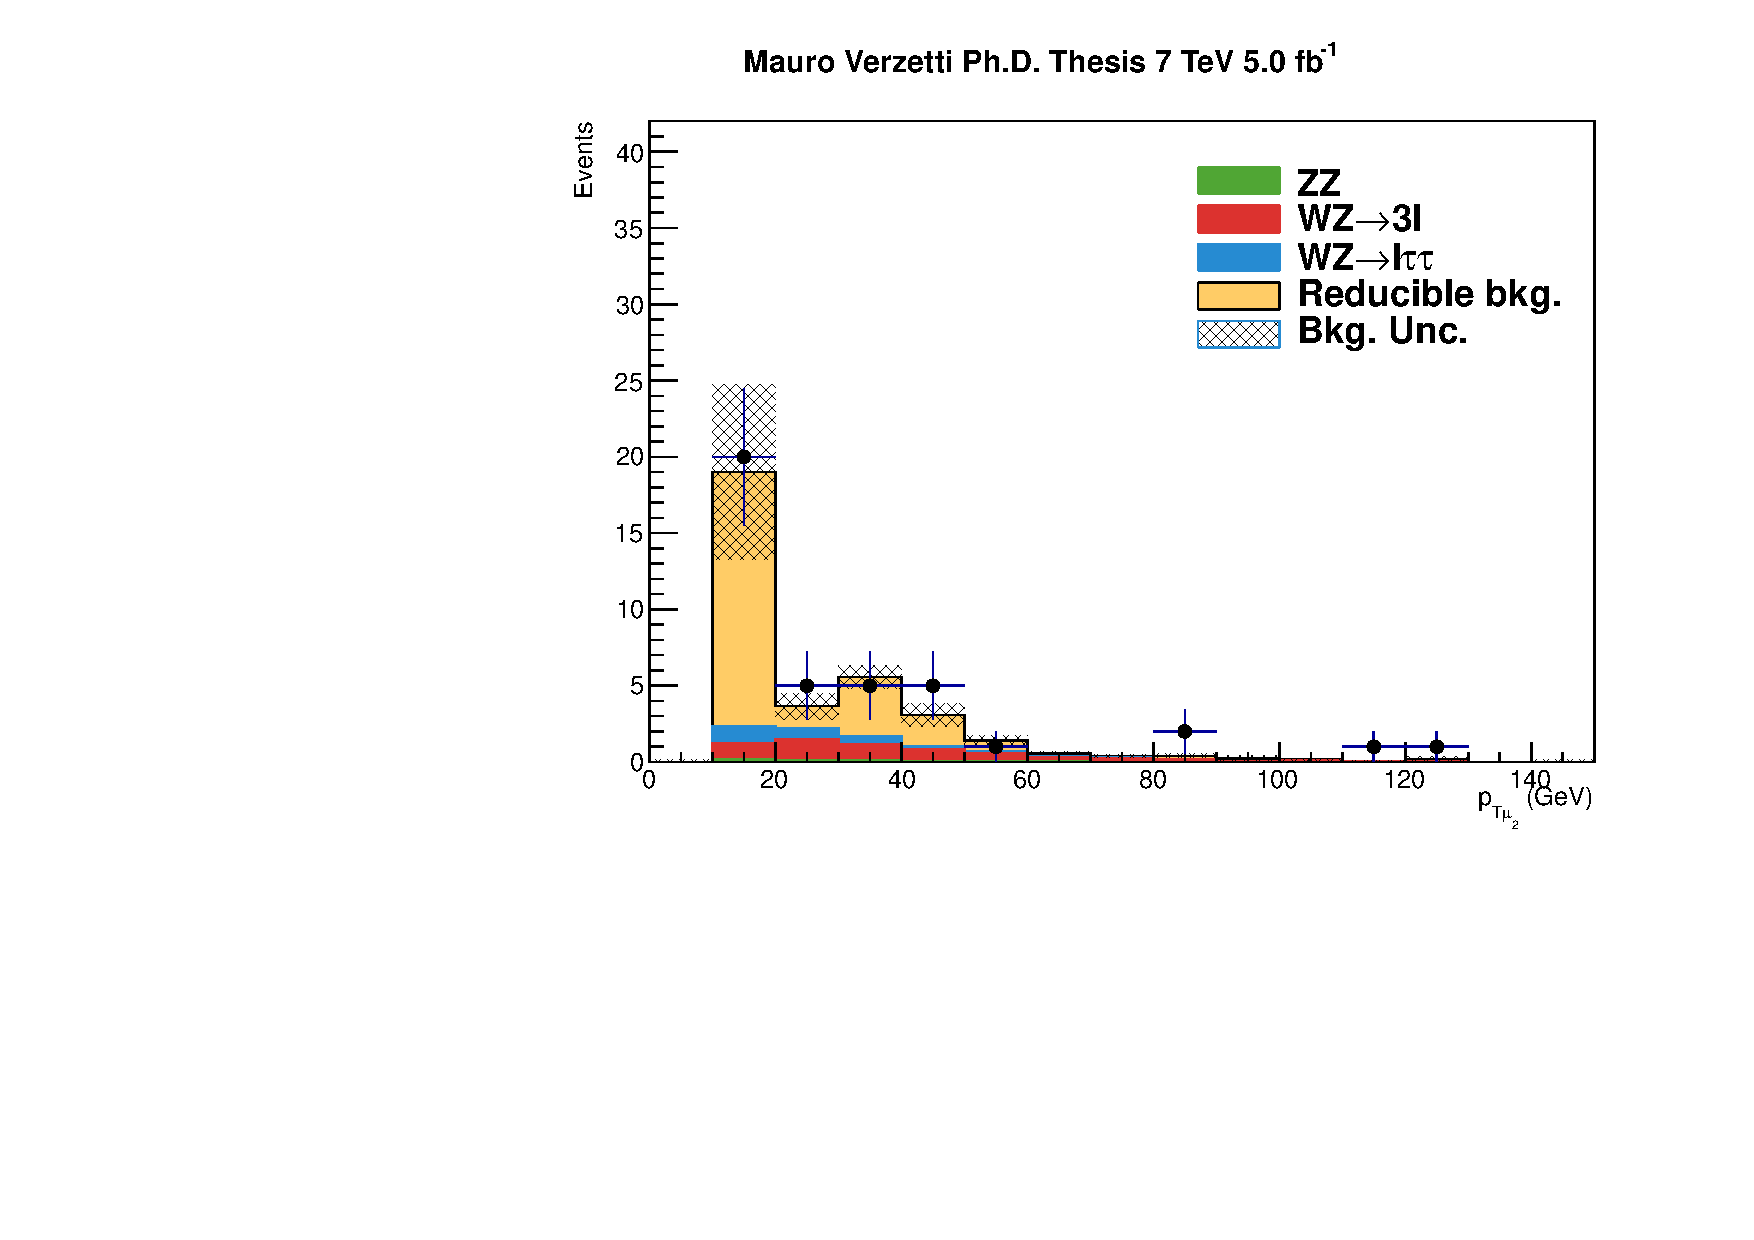
\includegraphics[width=0.49\textwidth]{4_Analisys/pics/7TeV/plots/mmt/f3/Full/final-f3-m2Pt-Full.pdf}\\
  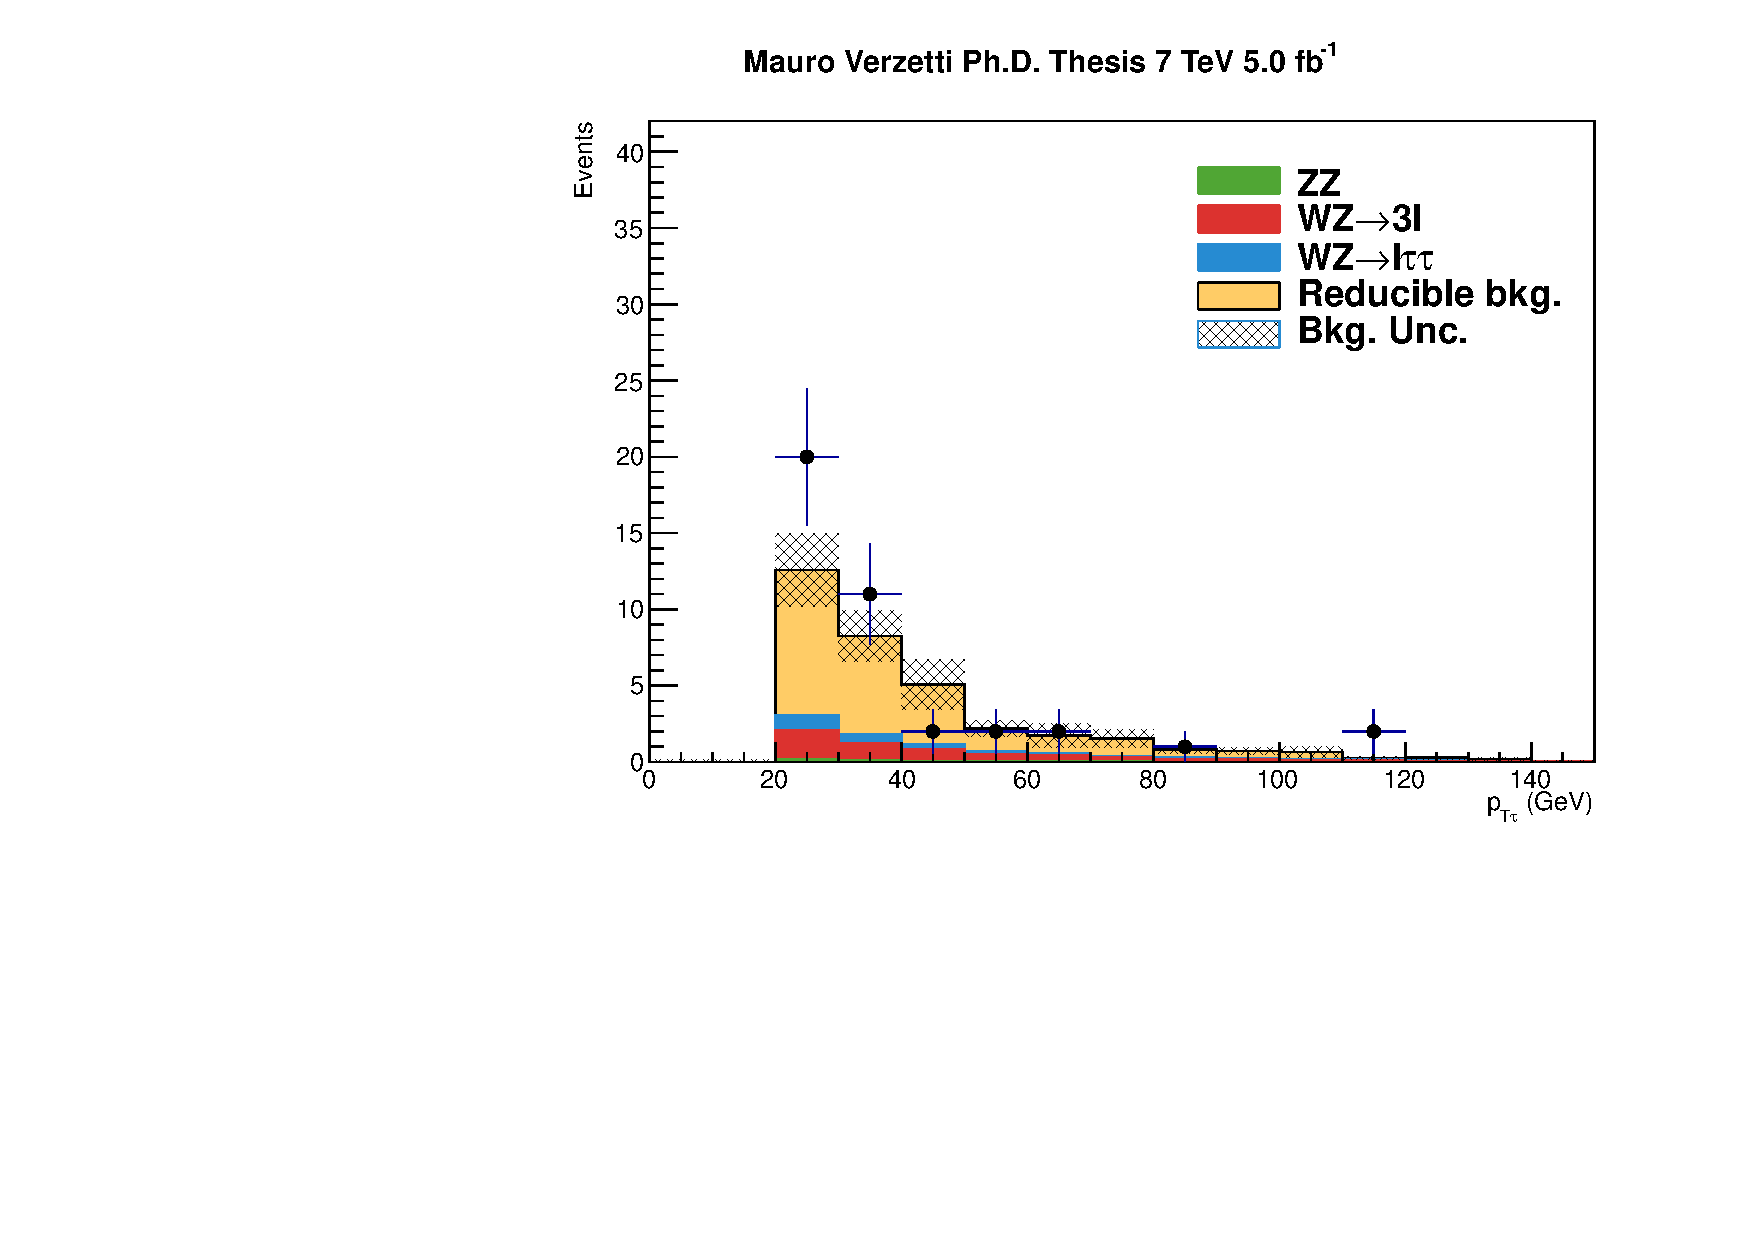
\includegraphics[width=0.49\textwidth]{4_Analisys/pics/7TeV/plots/mmt/f3/Full/final-f3-tPt-Full.pdf}
  \caption{Comparison of measured and predicted backgrounds in the $\mu\mu\tau_h$ ``fake tau'' control region for 7 TeV data.
  From top left to bottom: mass of the sub-leading muon and the tau system, scalar sum of the leptons \pT ($L_T$), \pT of the leading and sub-leading muon, and \pT of the hadronic tau.
  The non-prompt background estimate is computed in the same manner as that in the signal region.
  The shaded band represents the background uncertainty.
  }
  \label{fig:LLT_mmt_f3_control_7TeV}
\end{center}
\end{figure}

\begin{figure}
\begin{center}
  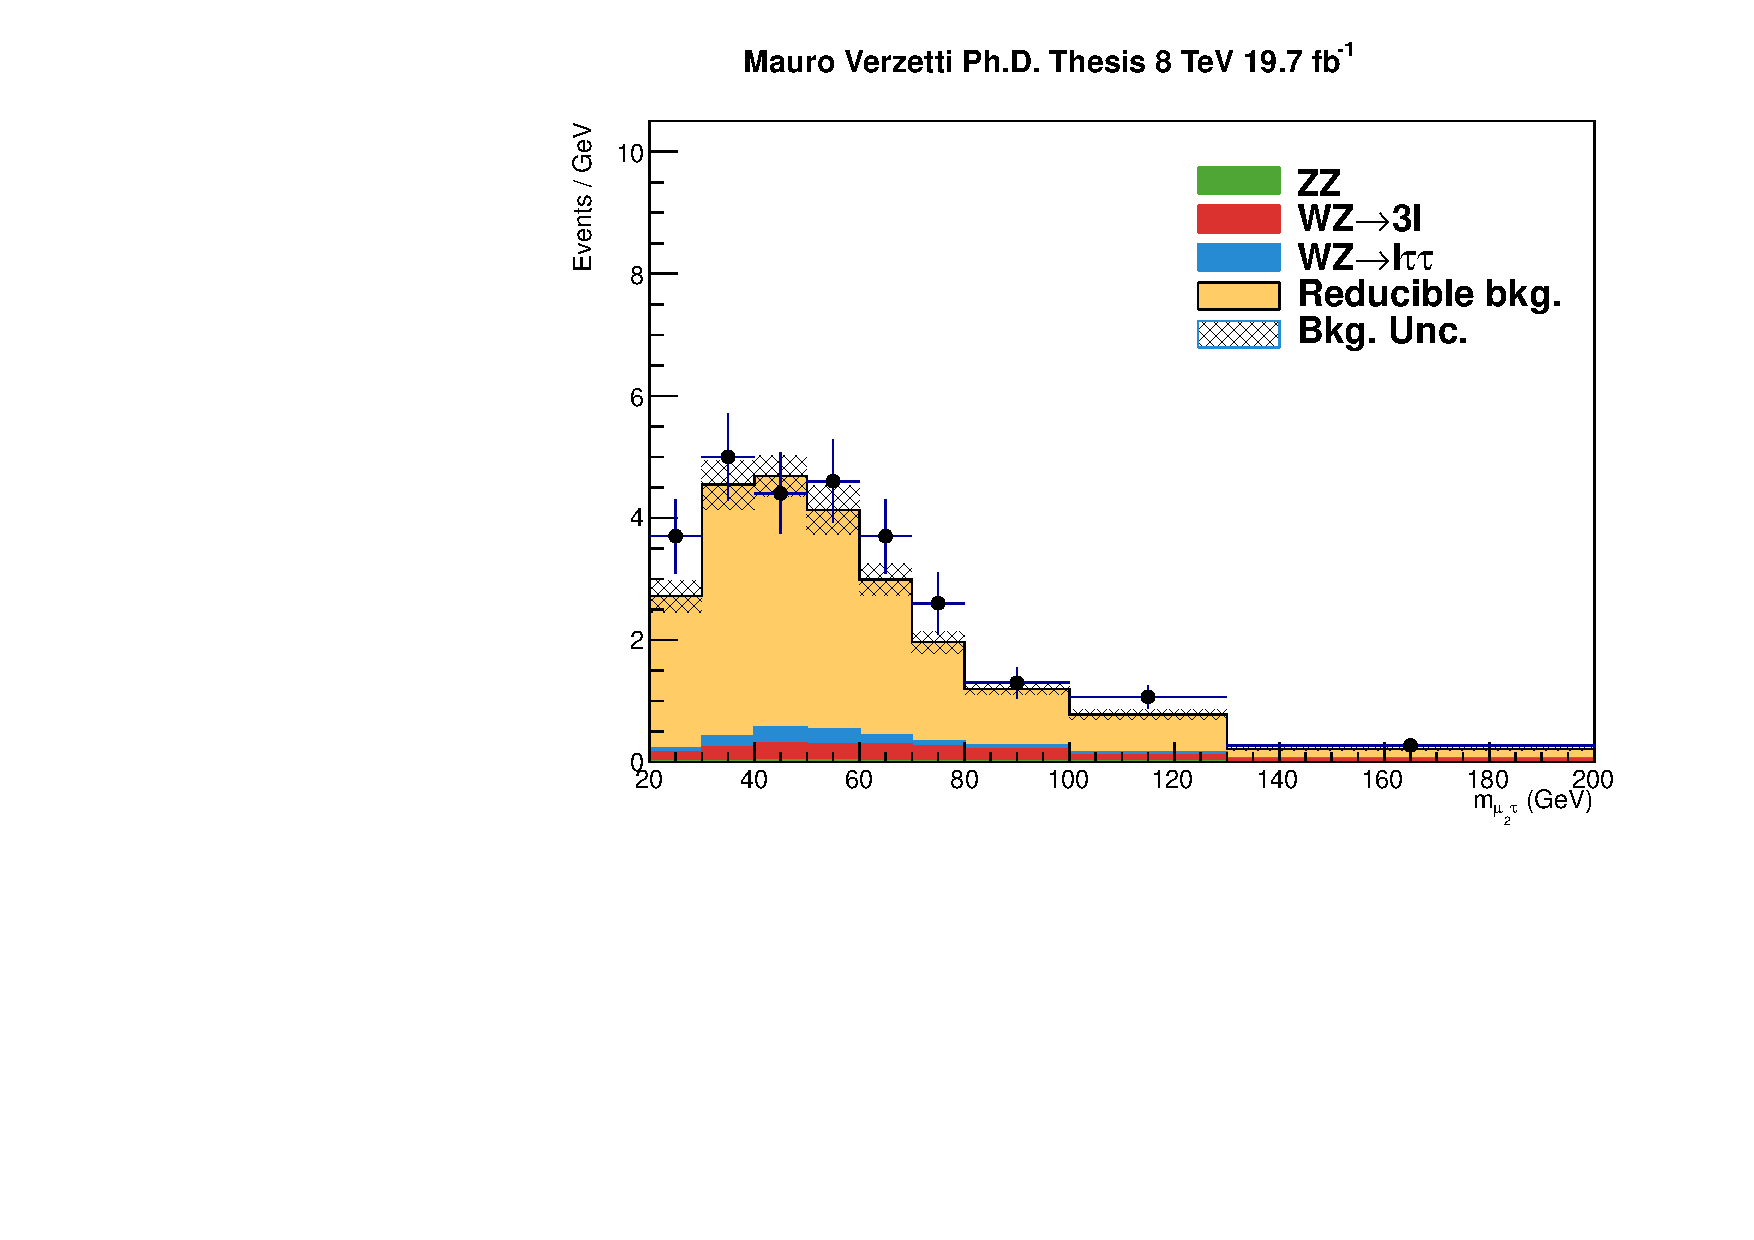
\includegraphics[width=0.49\textwidth]{4_Analisys/pics/8TeV/plots/mmt/f3/Full/final-f3-subMass-Full.pdf}
  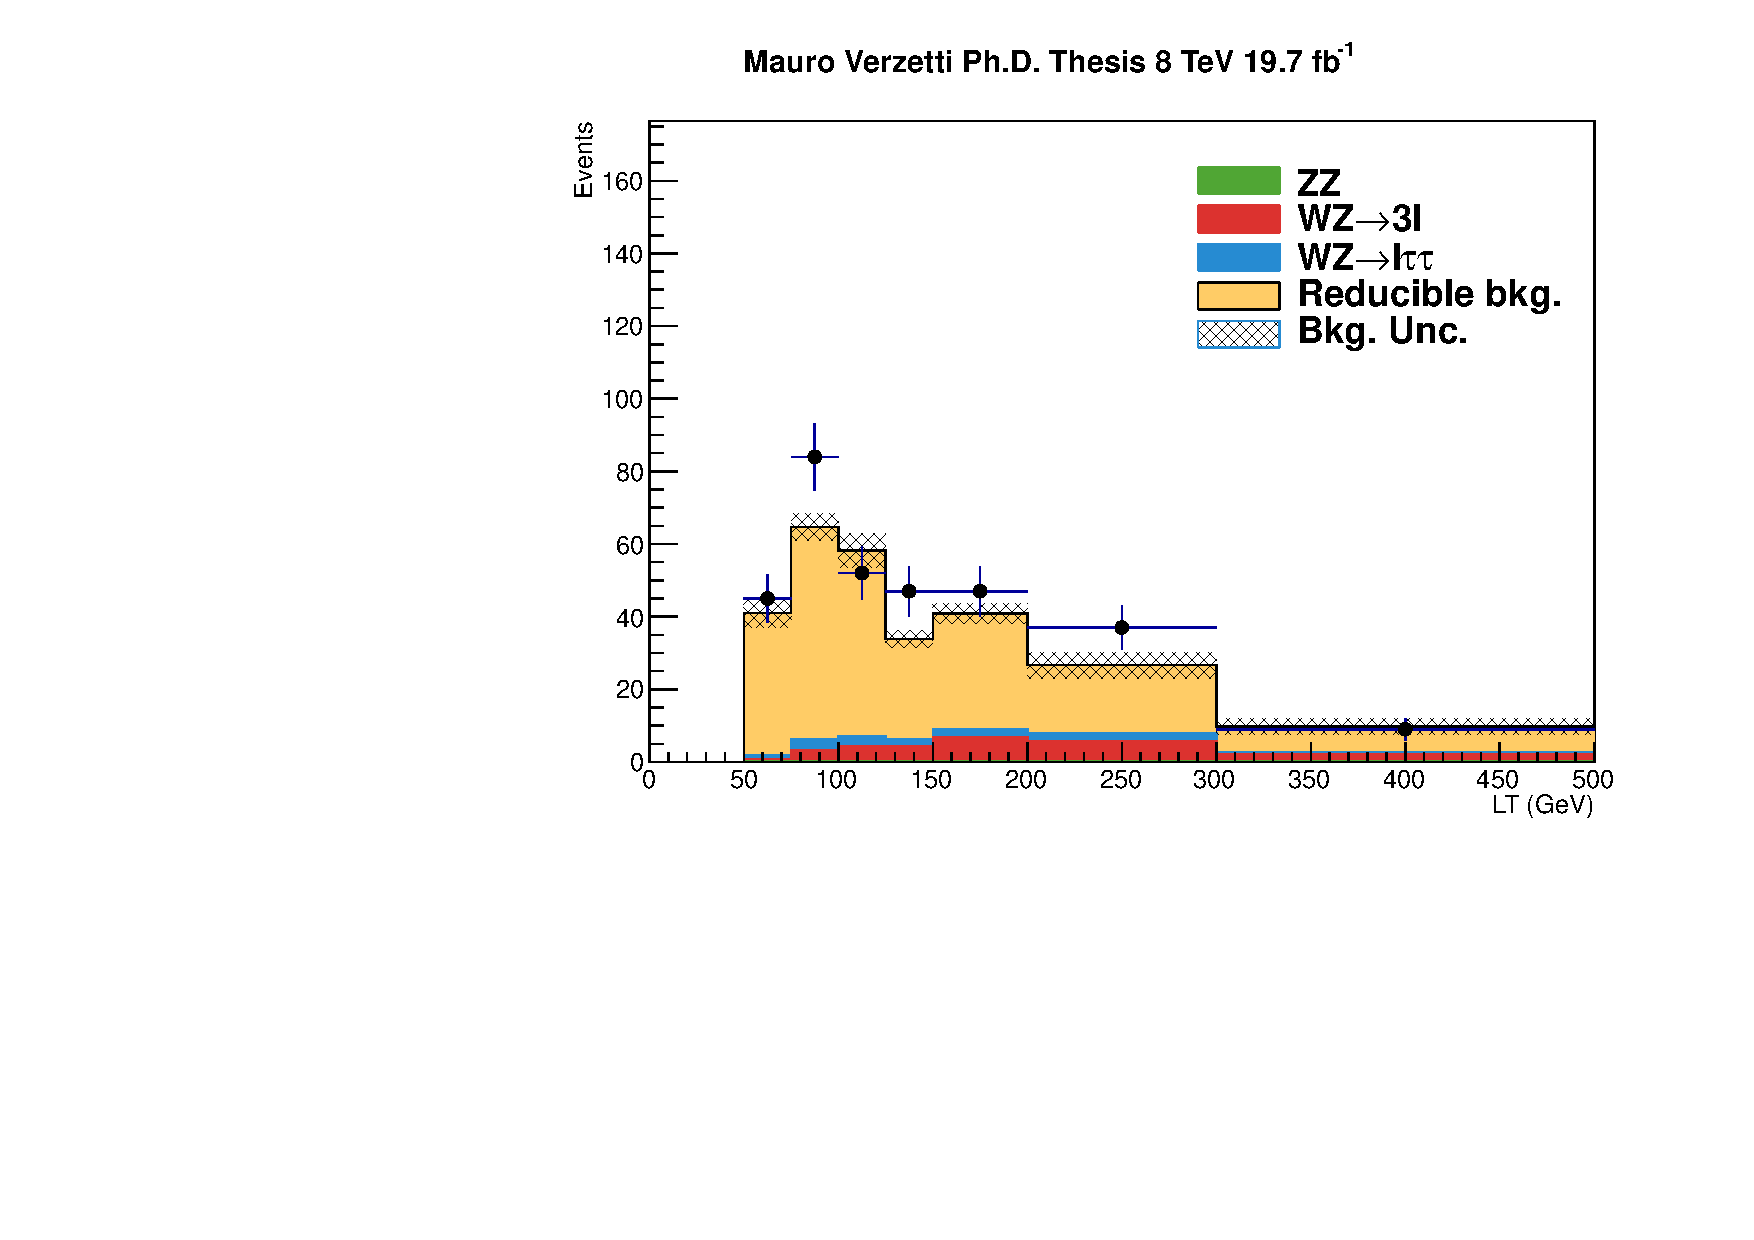
\includegraphics[width=0.49\textwidth]{4_Analisys/pics/8TeV/plots/mmt/f3/final-LT.pdf}\\
  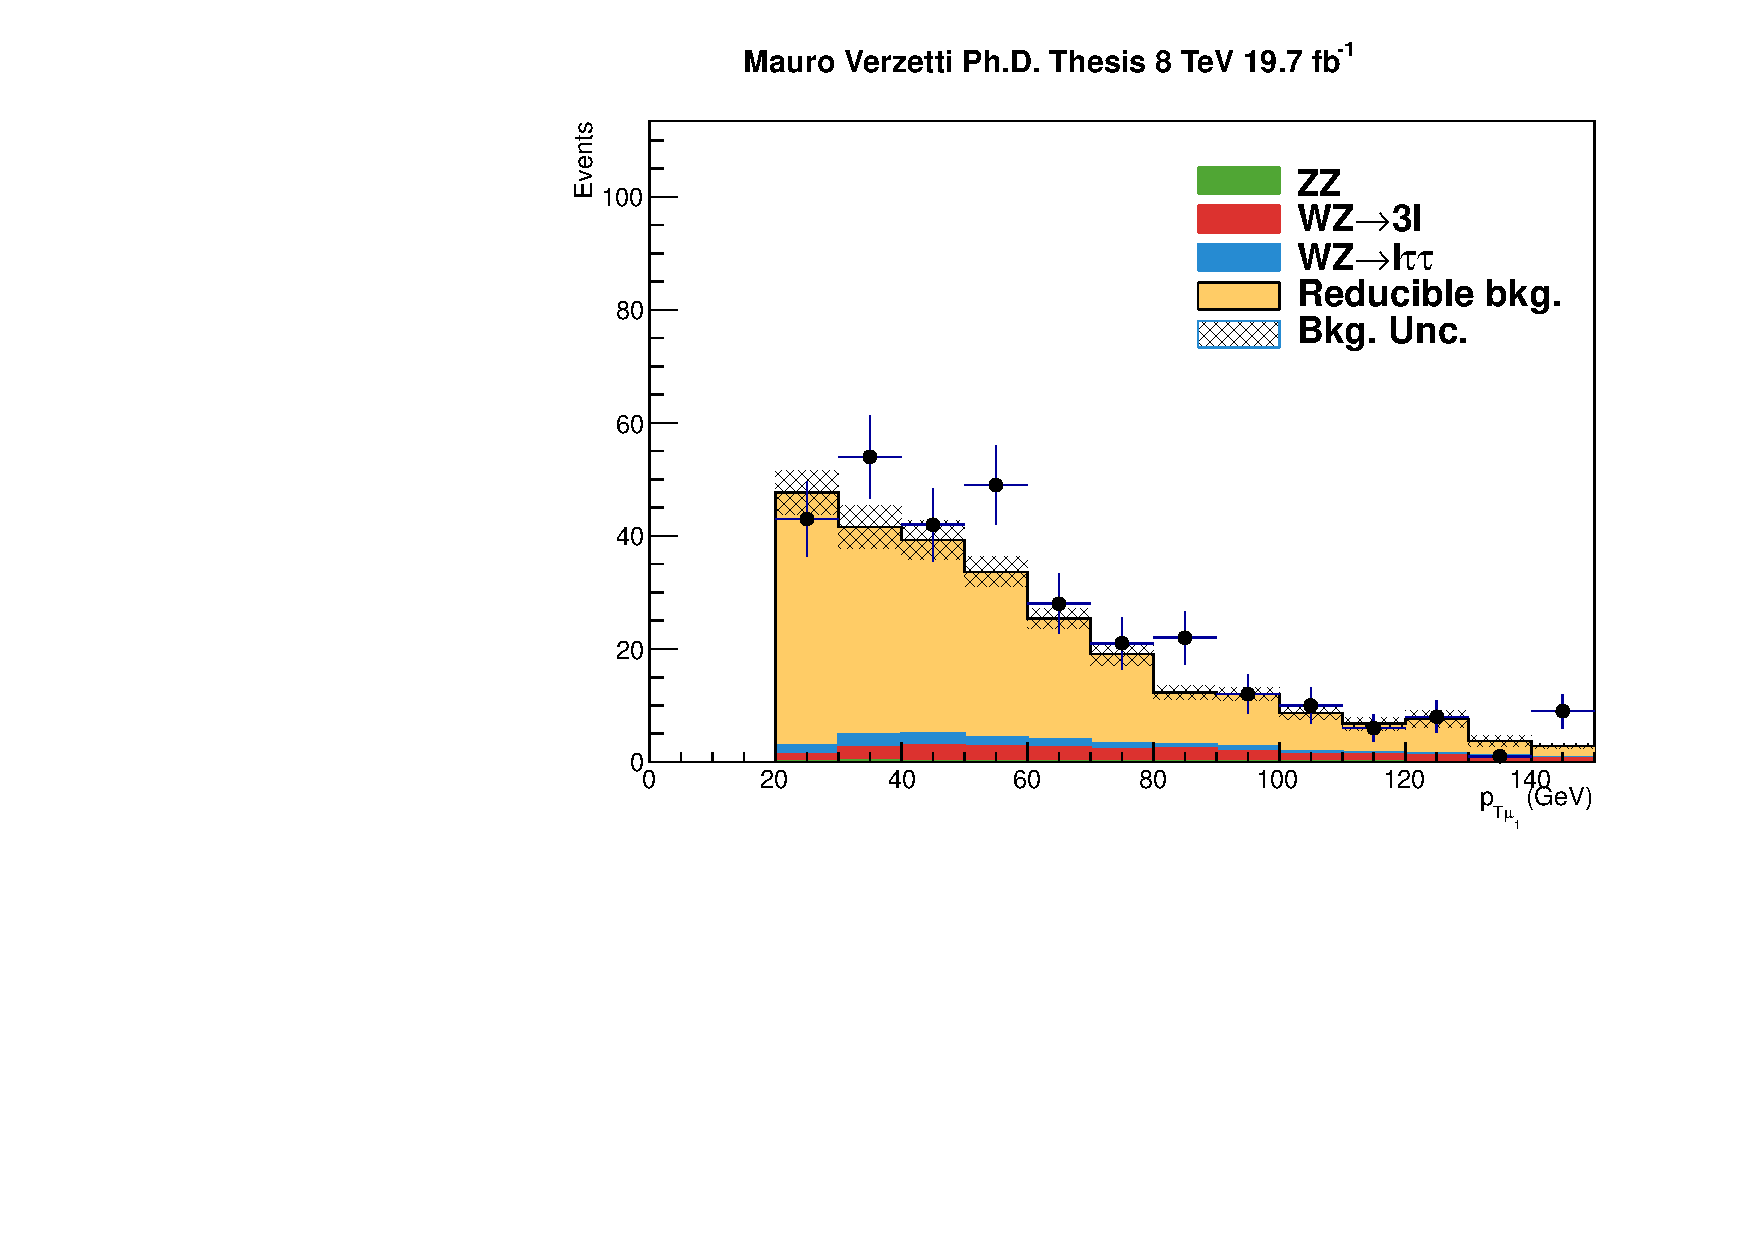
\includegraphics[width=0.49\textwidth]{4_Analisys/pics/8TeV/plots/mmt/f3/Full/final-f3-m1Pt-Full.pdf}
  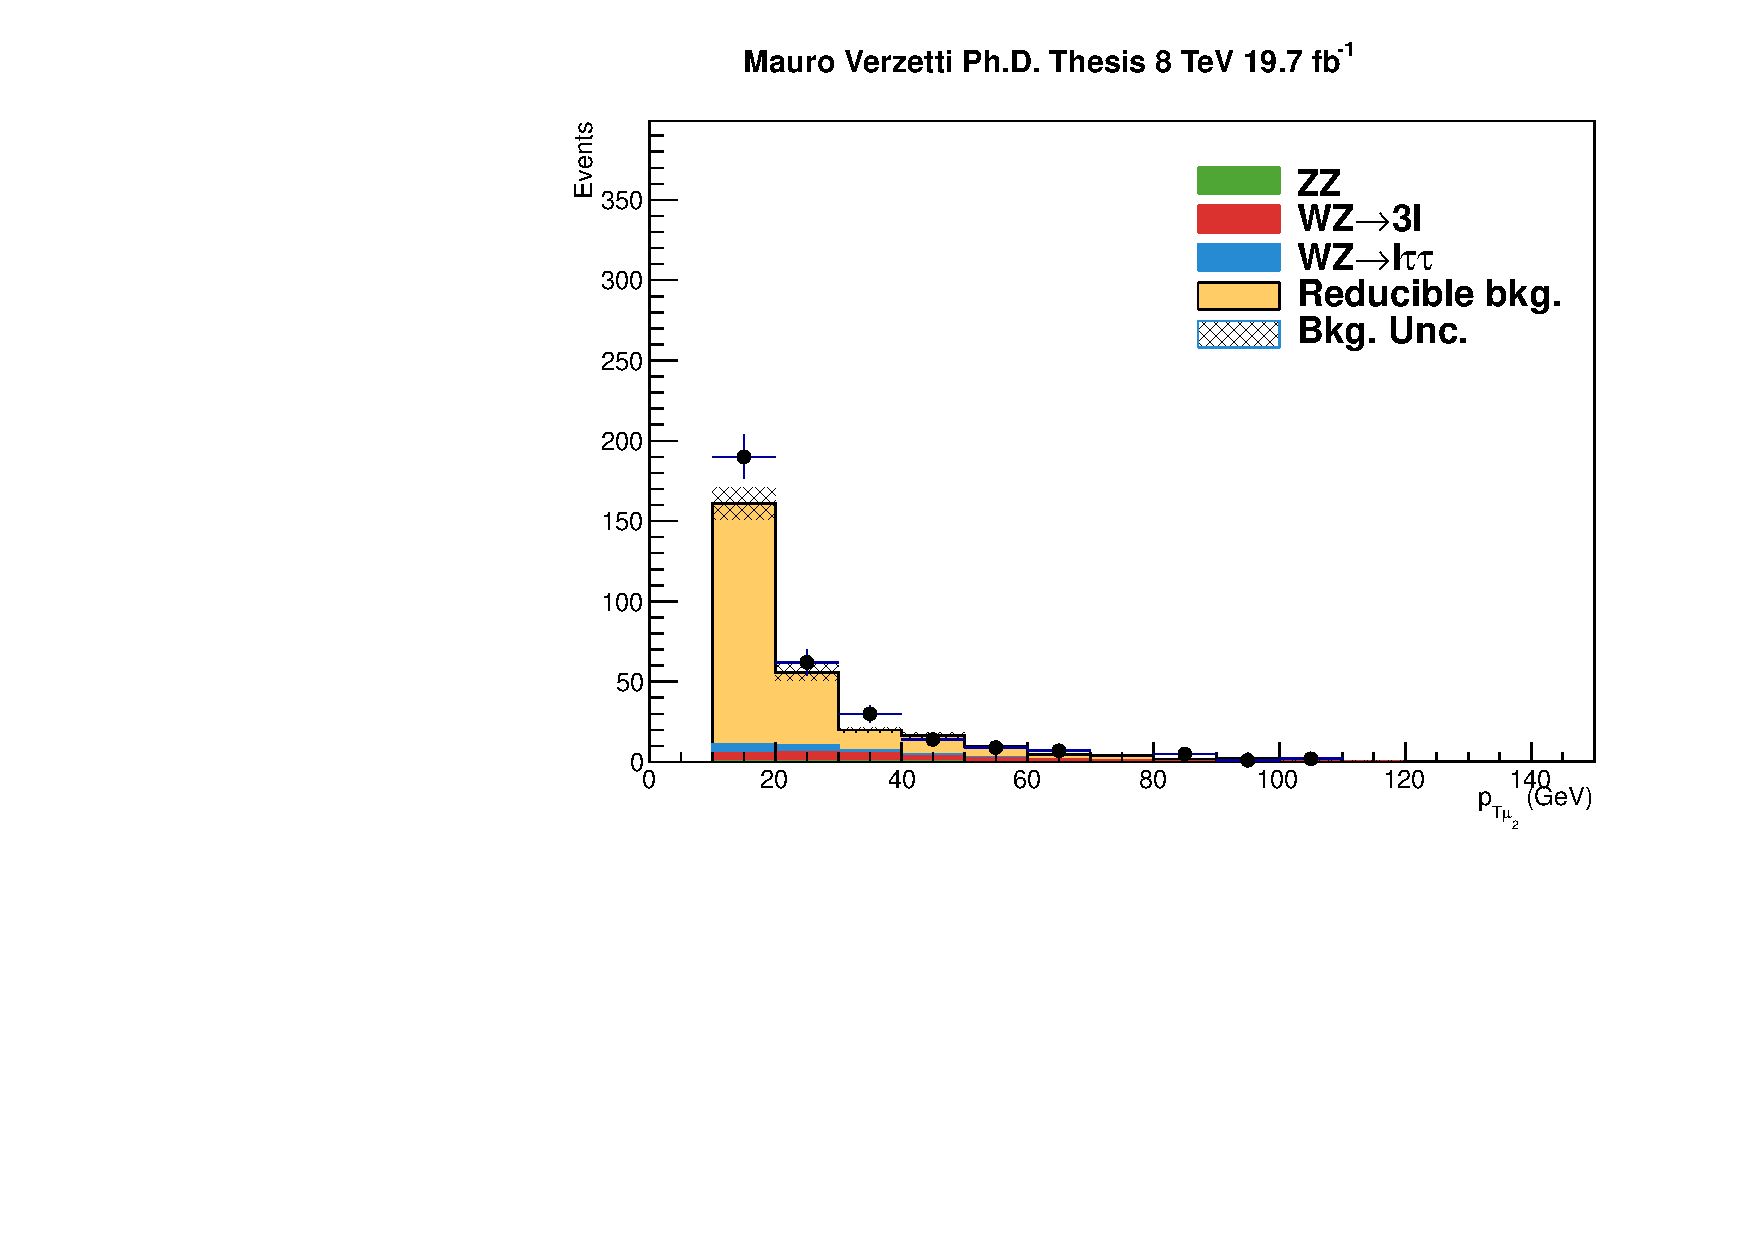
\includegraphics[width=0.49\textwidth]{4_Analisys/pics/8TeV/plots/mmt/f3/Full/final-f3-m2Pt-Full.pdf}\\
  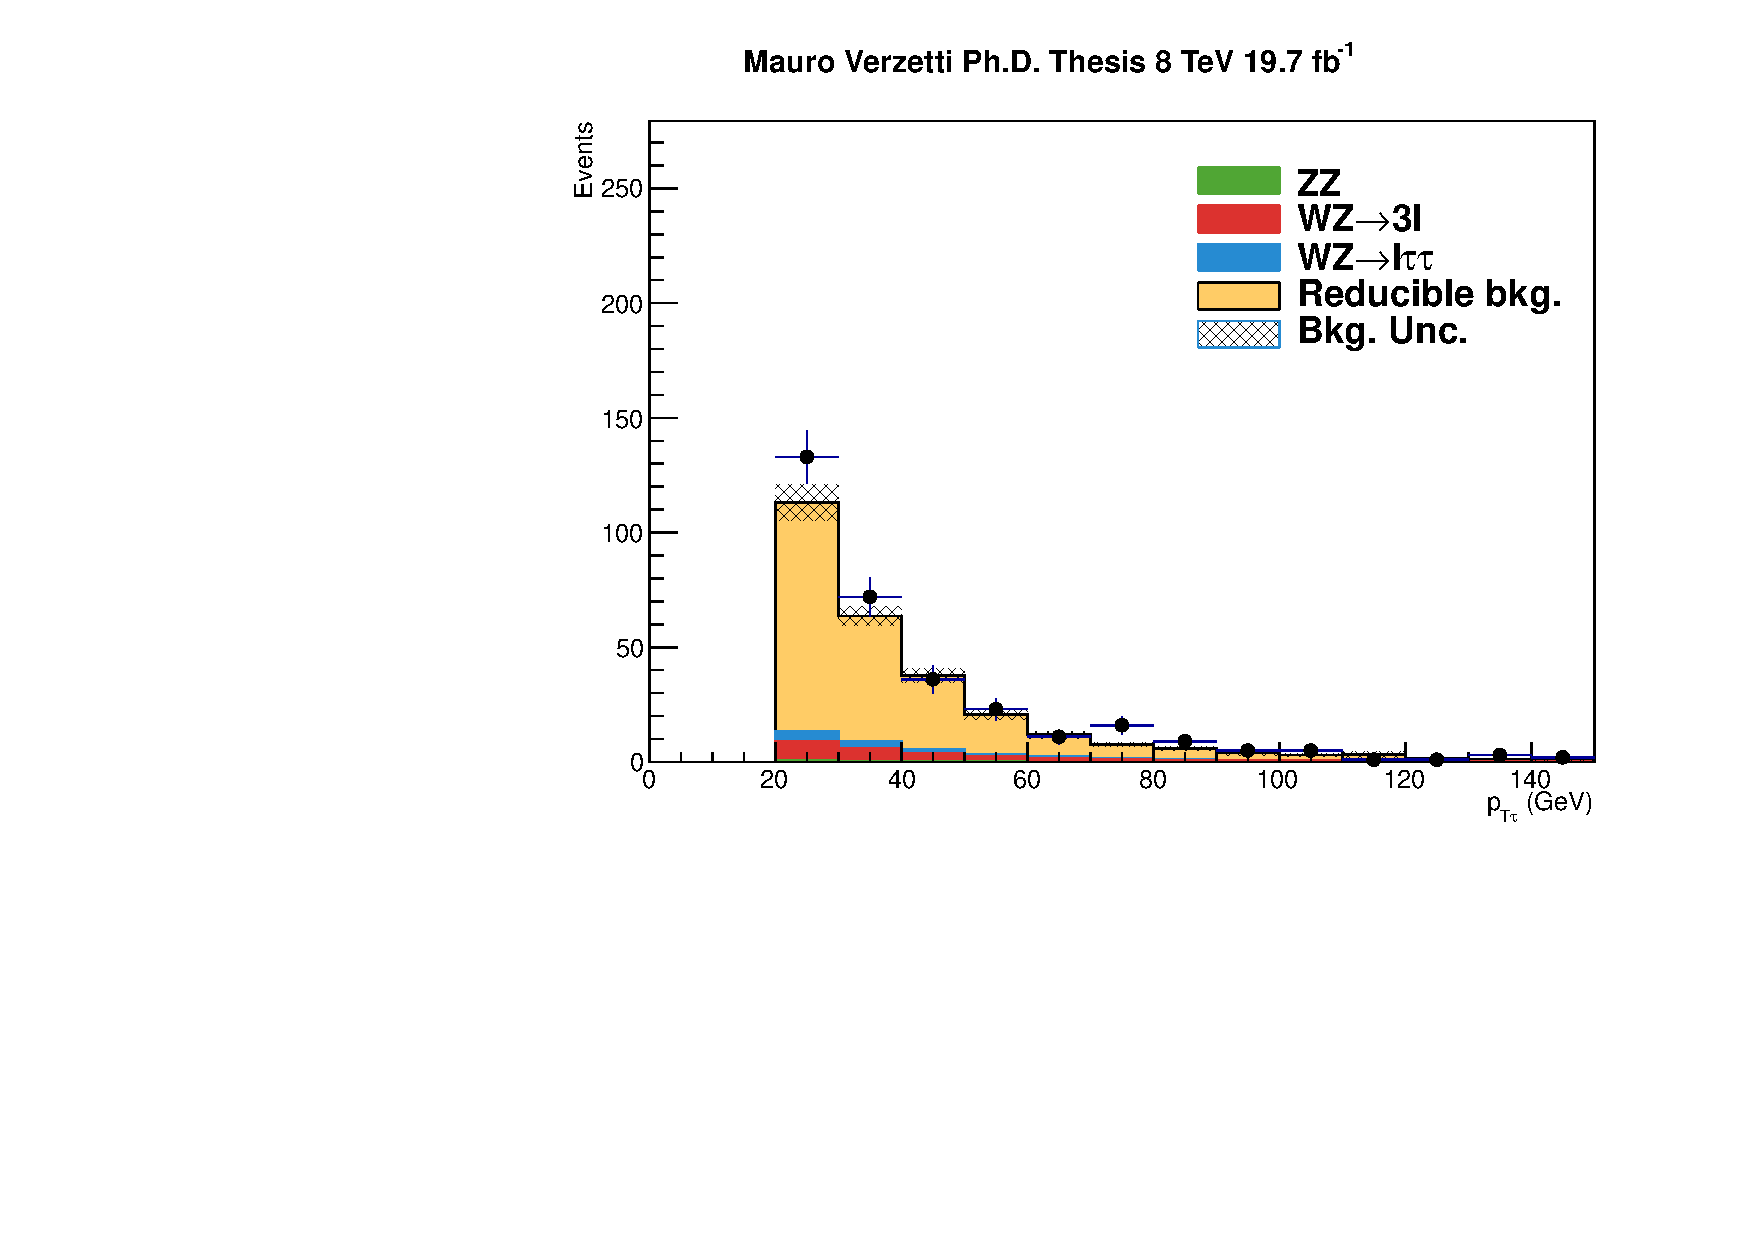
\includegraphics[width=0.49\textwidth]{4_Analisys/pics/8TeV/plots/mmt/f3/Full/final-f3-tPt-Full.pdf}
  \caption{Comparison of measured and predicted backgrounds in the $\mu\mu\tau_h$ ``fake tau'' control region for 8 TeV data.
  From top left to bottom: mass of the sub-leading muon and the tau system, scalar sum of the leptons \pT ($L_T$), \pT of the leading and sub-leading muon, and \pT of the hadronic tau.
  The non-prompt background estimate is computed in the same manner as that in the signal region.
  The shaded band represents the background uncertainty.
  }
  \label{fig:LLT_mmt_f3_control_8TeV}
\end{center}
\end{figure}

\begin{figure}
\begin{center}
  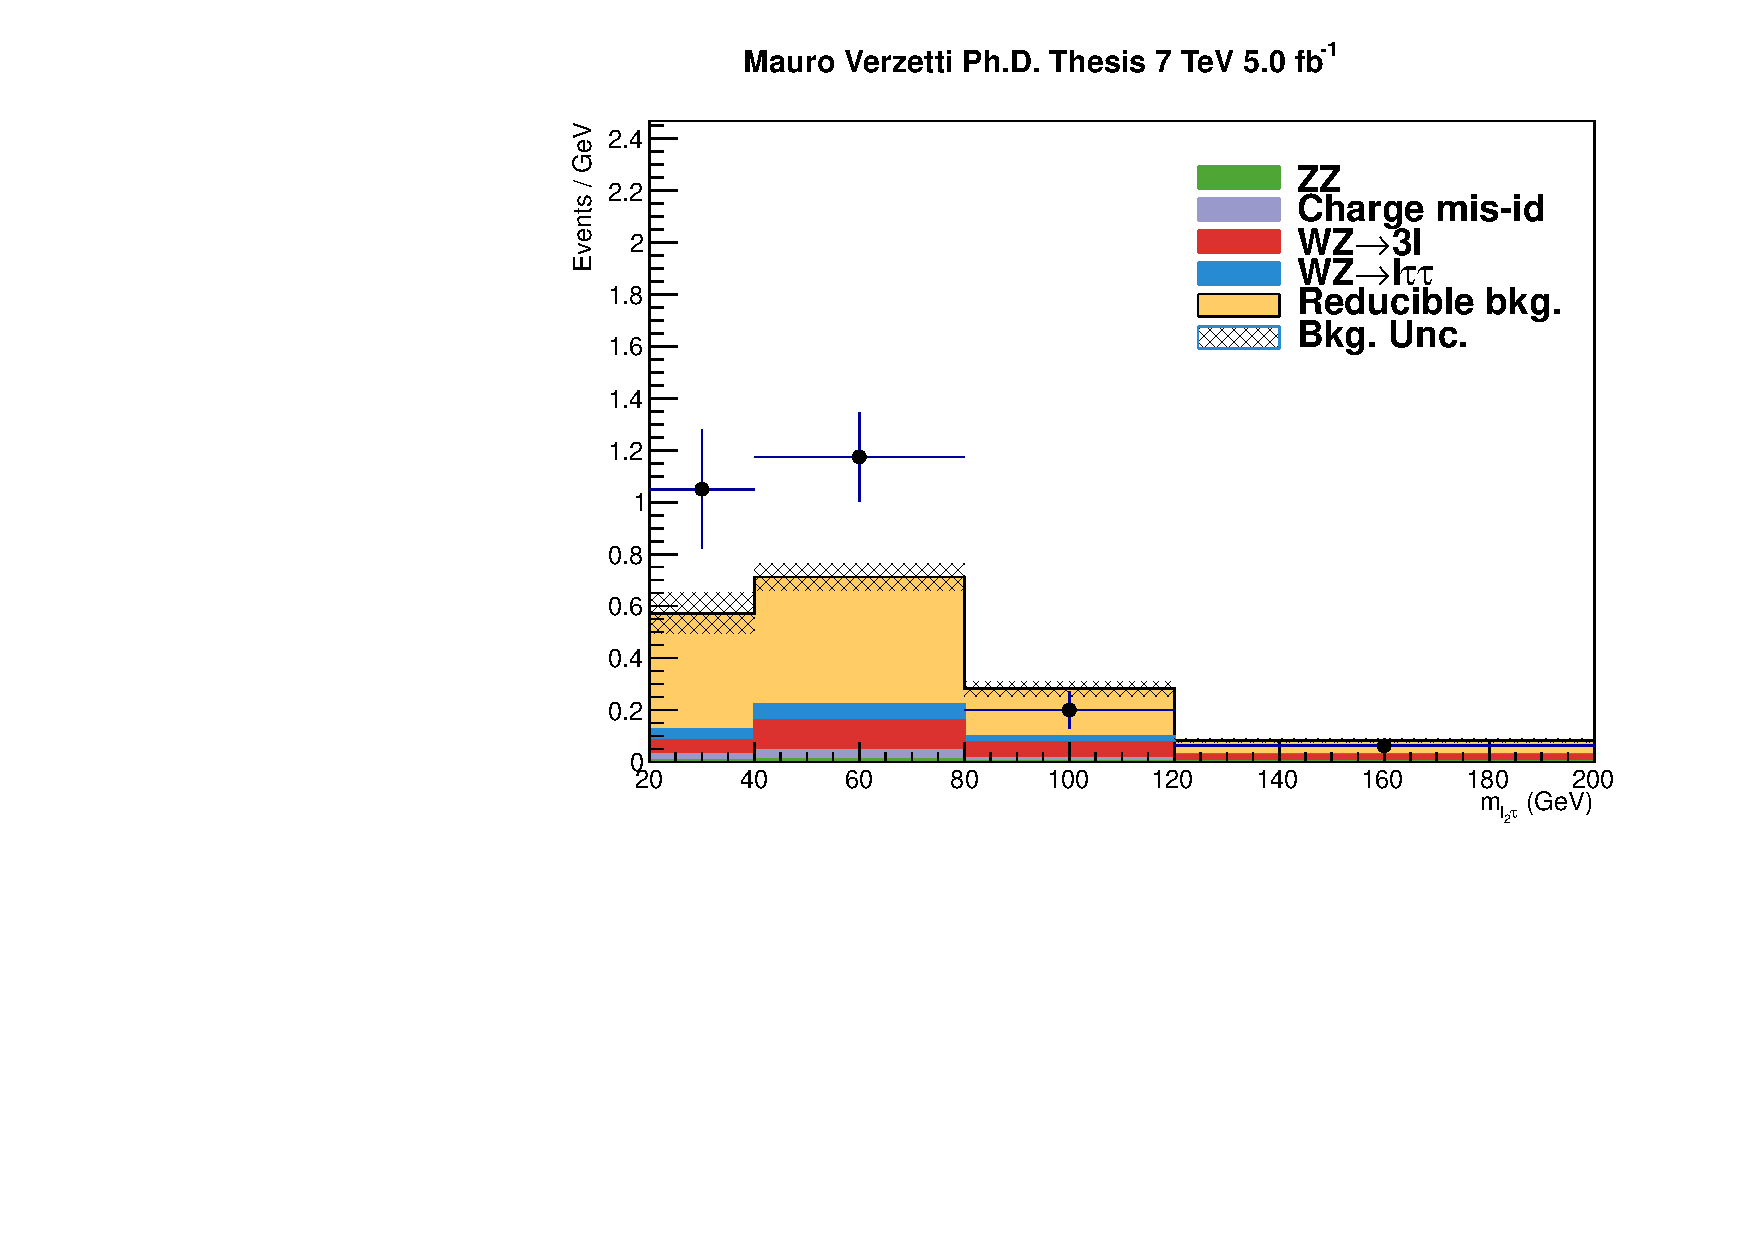
\includegraphics[width=0.49\textwidth]{4_Analisys/pics/7TeV/plots/emt/f3/Full/final-f3-subMass-Full.pdf}
  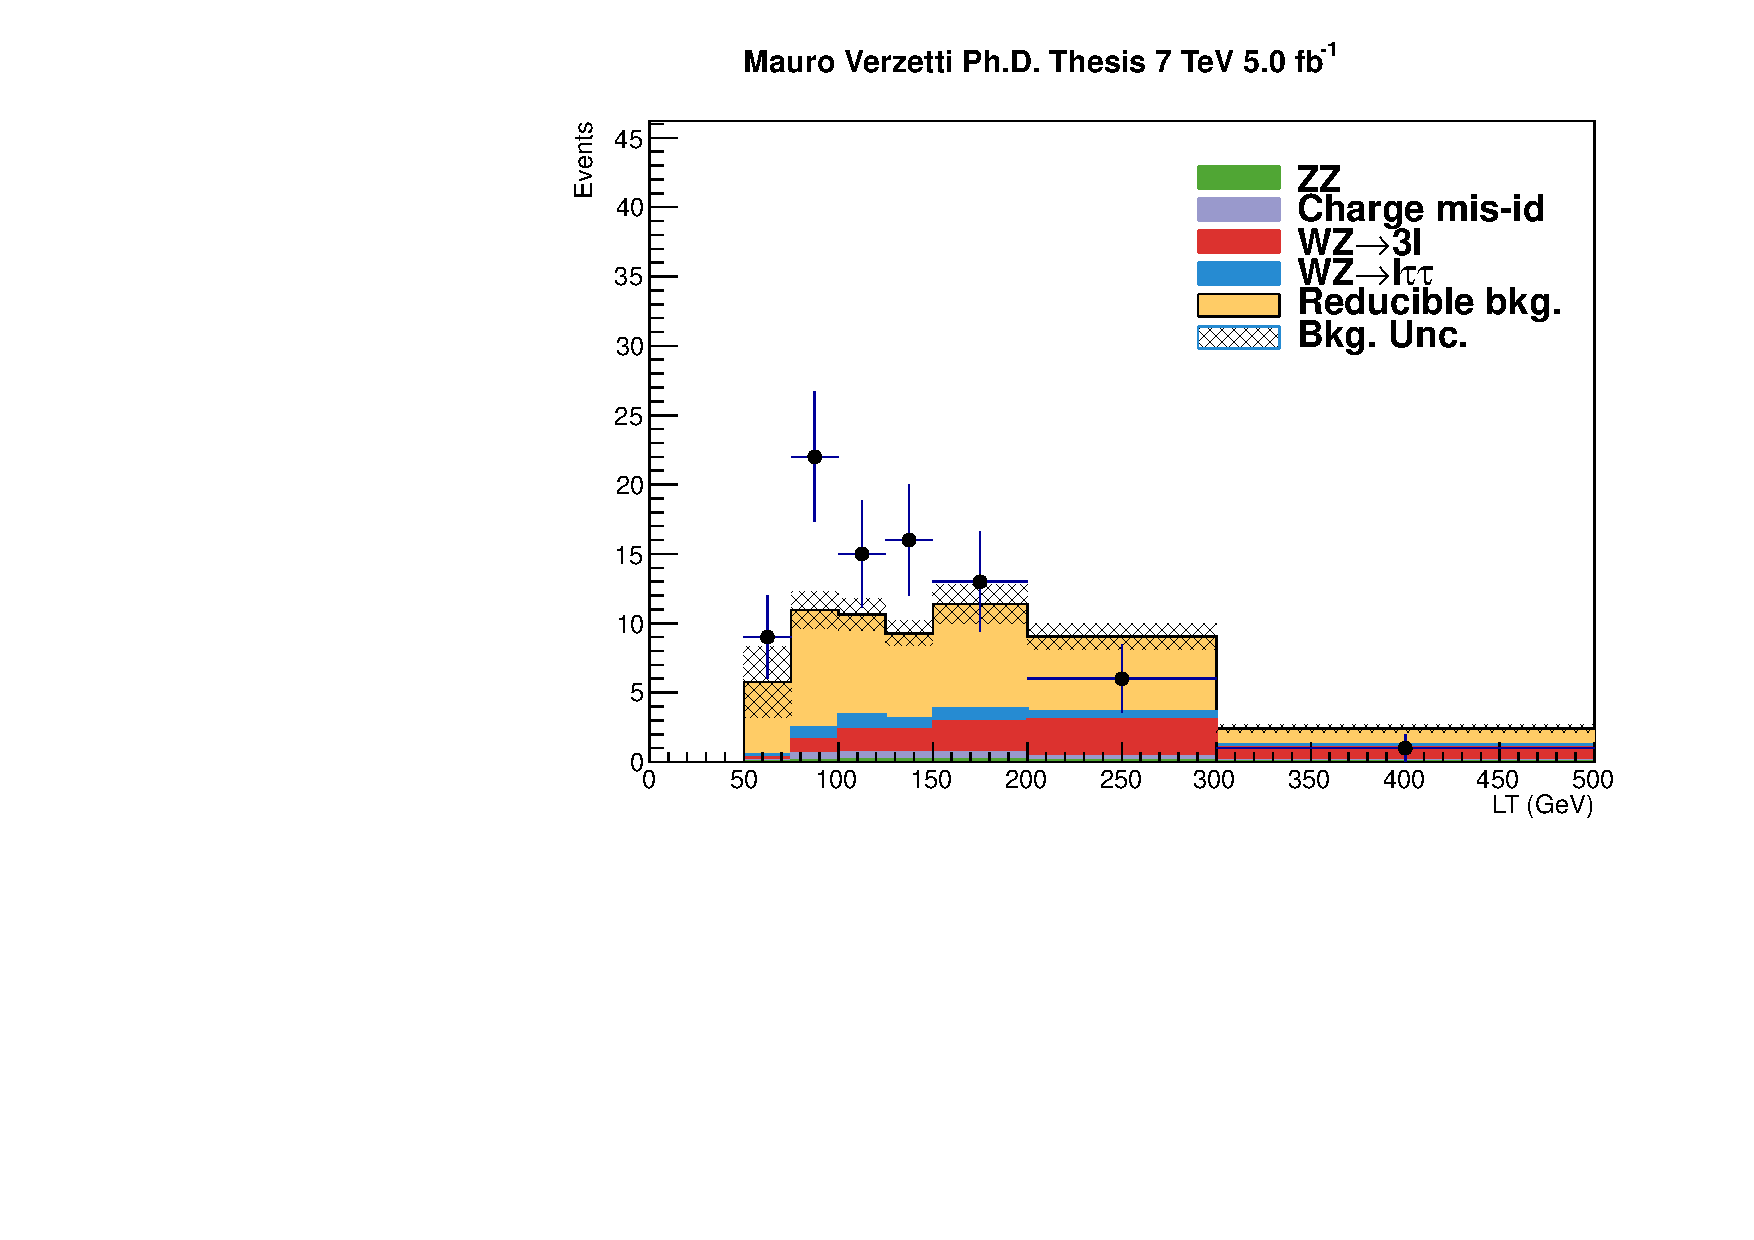
\includegraphics[width=0.49\textwidth]{4_Analisys/pics/7TeV/plots/emt/f3/final-f3-LT.pdf}\\
  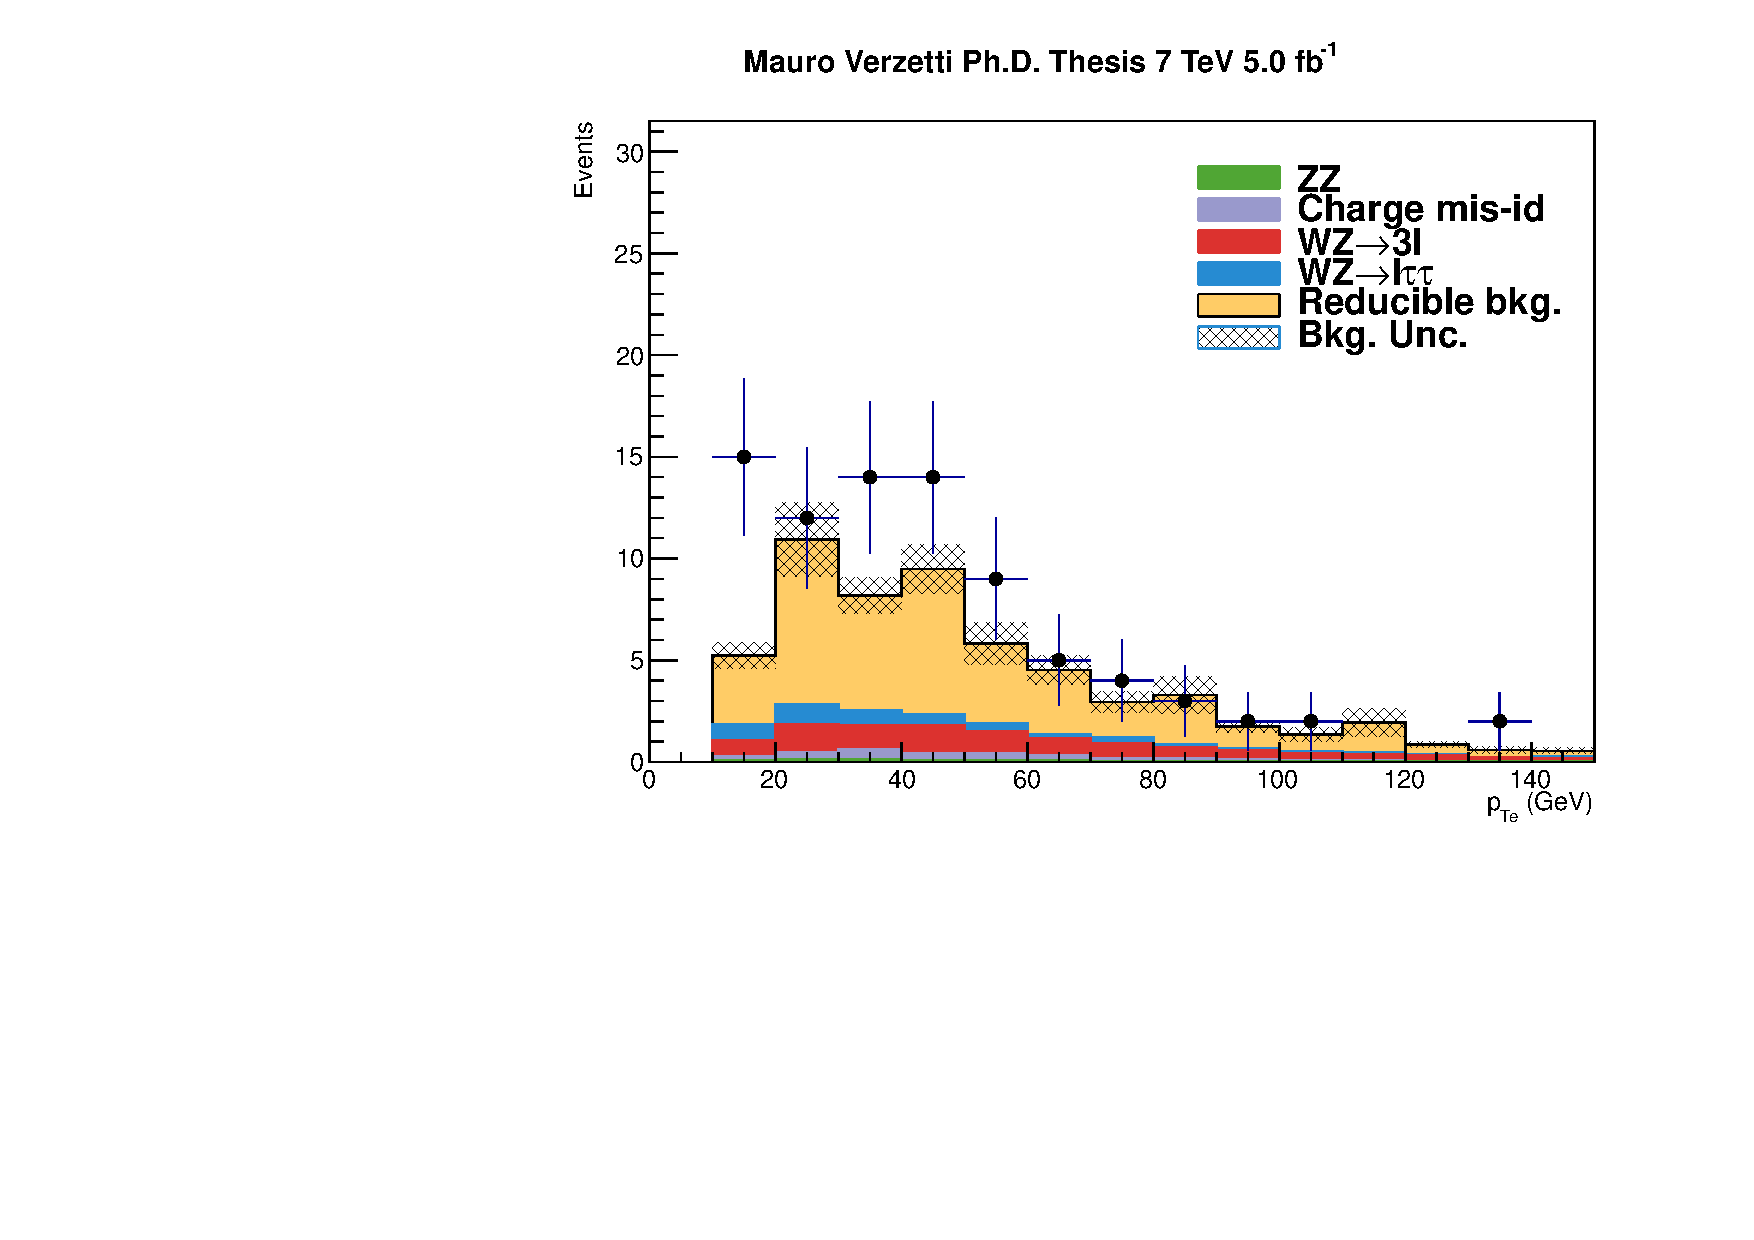
\includegraphics[width=0.49\textwidth]{4_Analisys/pics/7TeV/plots/emt/f3/Full/final-f3-ePt-Full.pdf}
  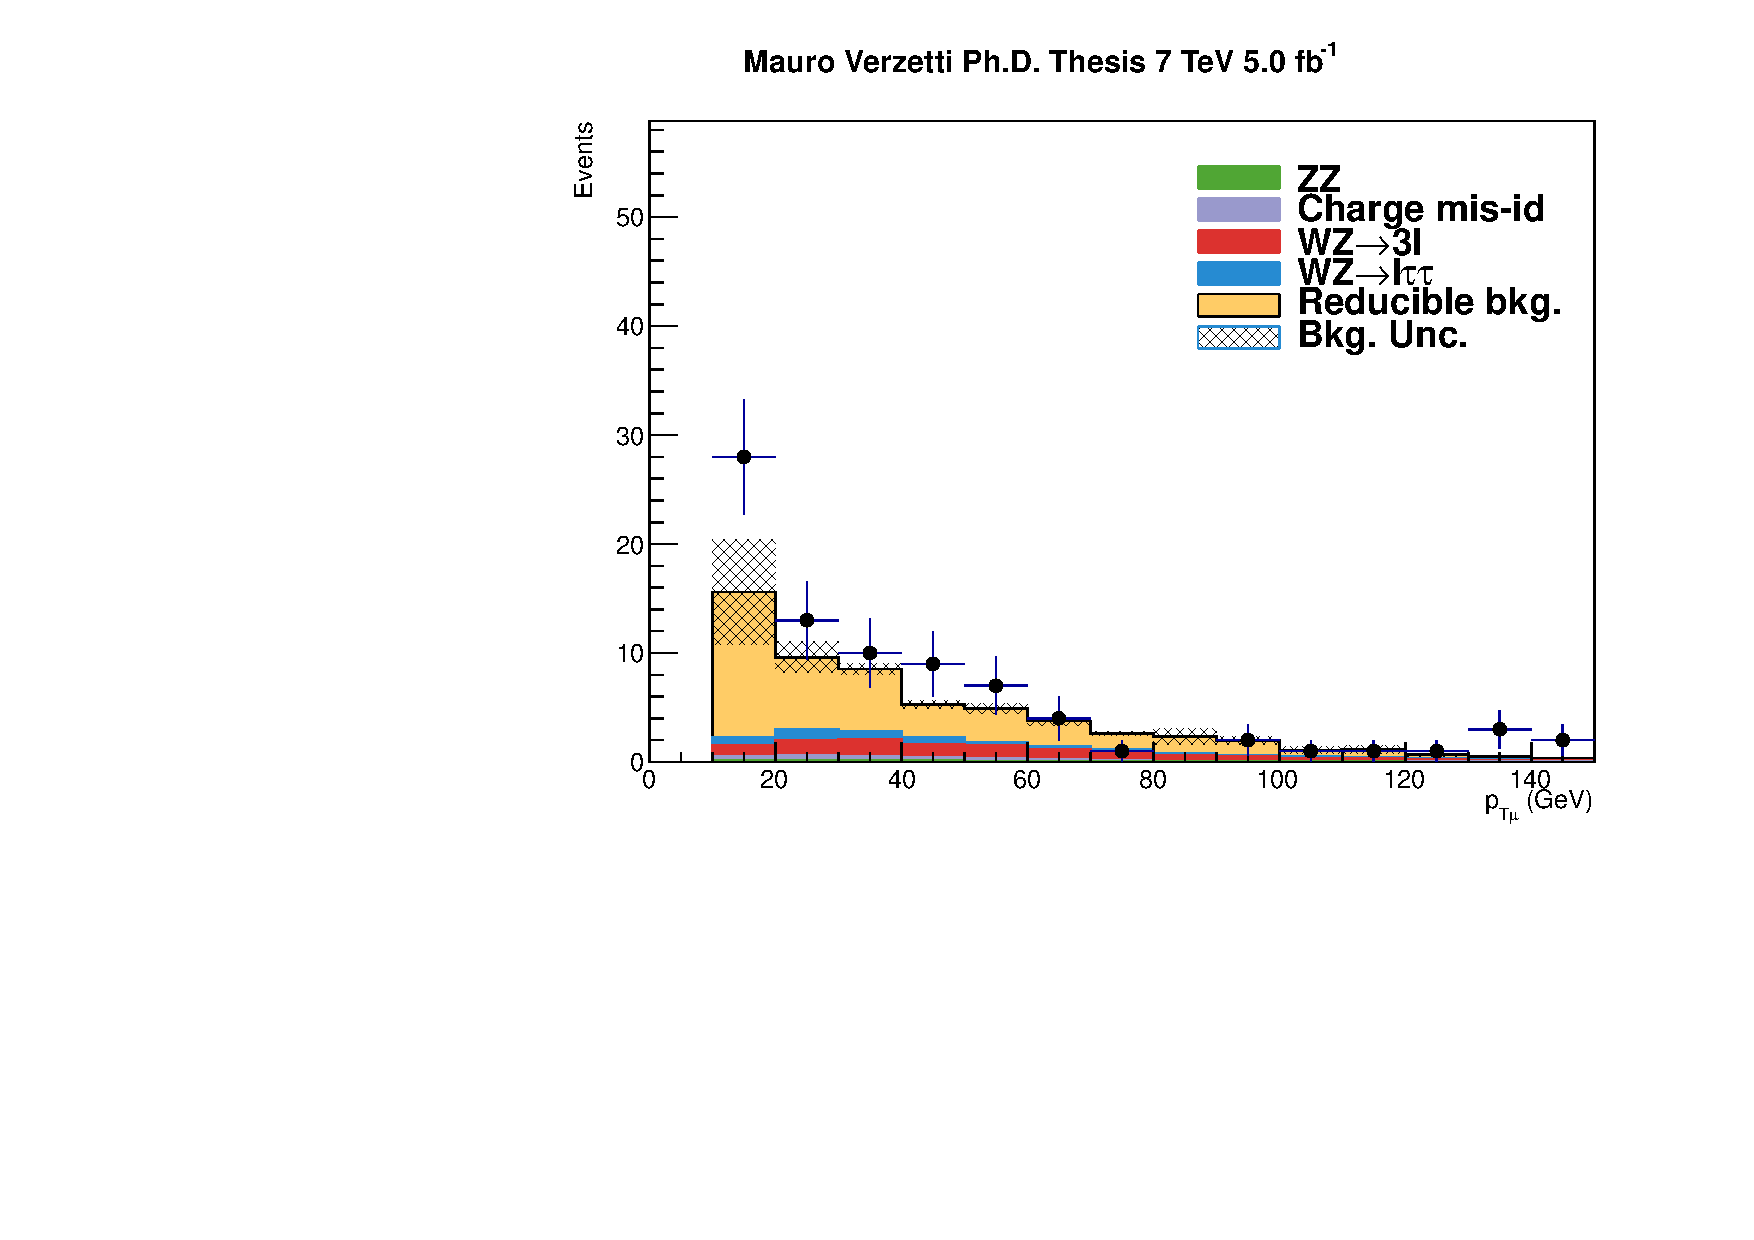
\includegraphics[width=0.49\textwidth]{4_Analisys/pics/7TeV/plots/emt/f3/Full/final-f3-mPt-Full.pdf}\\
  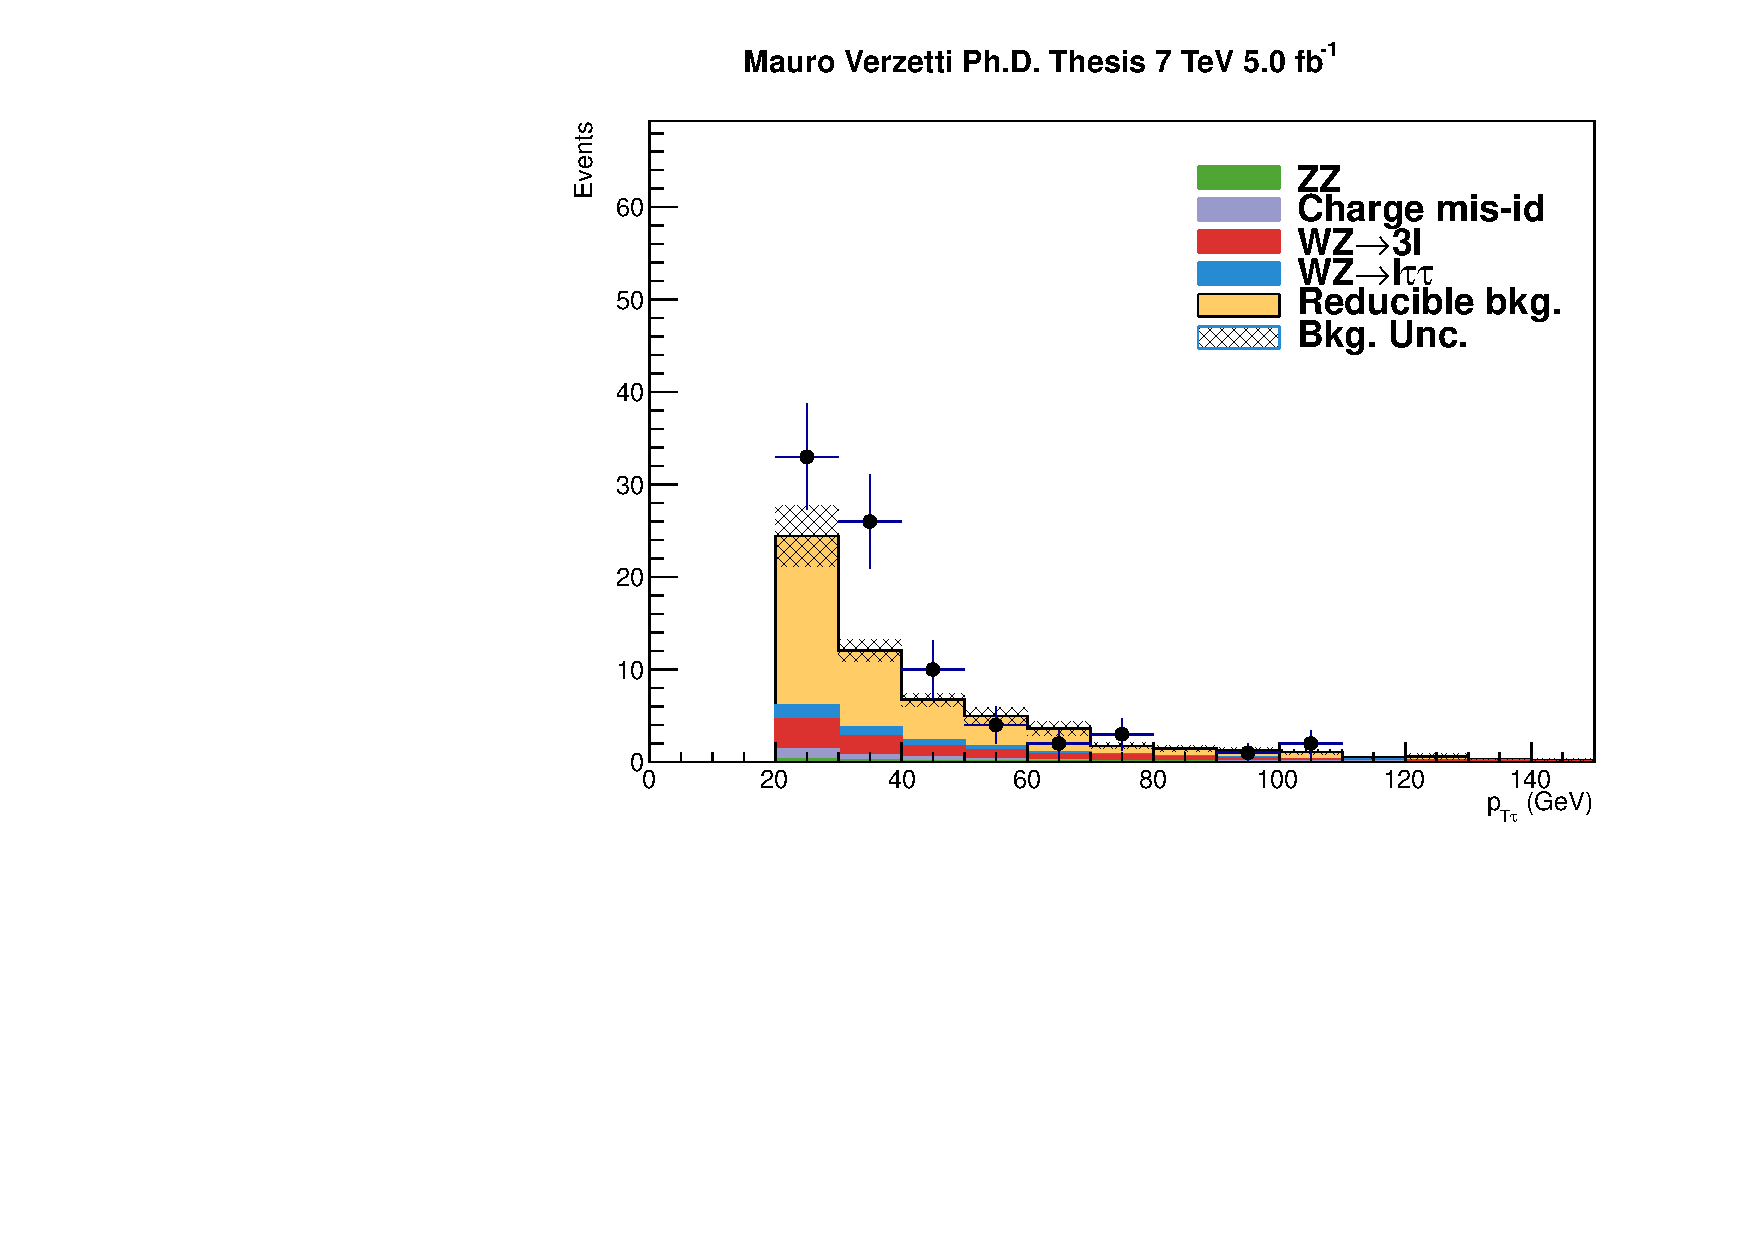
\includegraphics[width=0.49\textwidth]{4_Analisys/pics/7TeV/plots/emt/f3/Full/final-f3-tPt-Full.pdf}
  \caption{Comparison of measured and predicted backgrounds in the $e\mu\tau_h$ ``fake tau'' control region for 7 TeV data.
  From top left to bottom: mass of the sub-leading lepton and the tau system, scalar sum of the leptons \pT ($L_T$), \pT of the electron, muon, and hadronic tau.
  The non-prompt background estimate is computed in the same manner as that in the signal region.
  The shaded band represents the background uncertainty.
  }
  \label{fig:LLT_emt_f3_control_7TeV}
\end{center}
\end{figure}

\begin{figure}
\begin{center}
  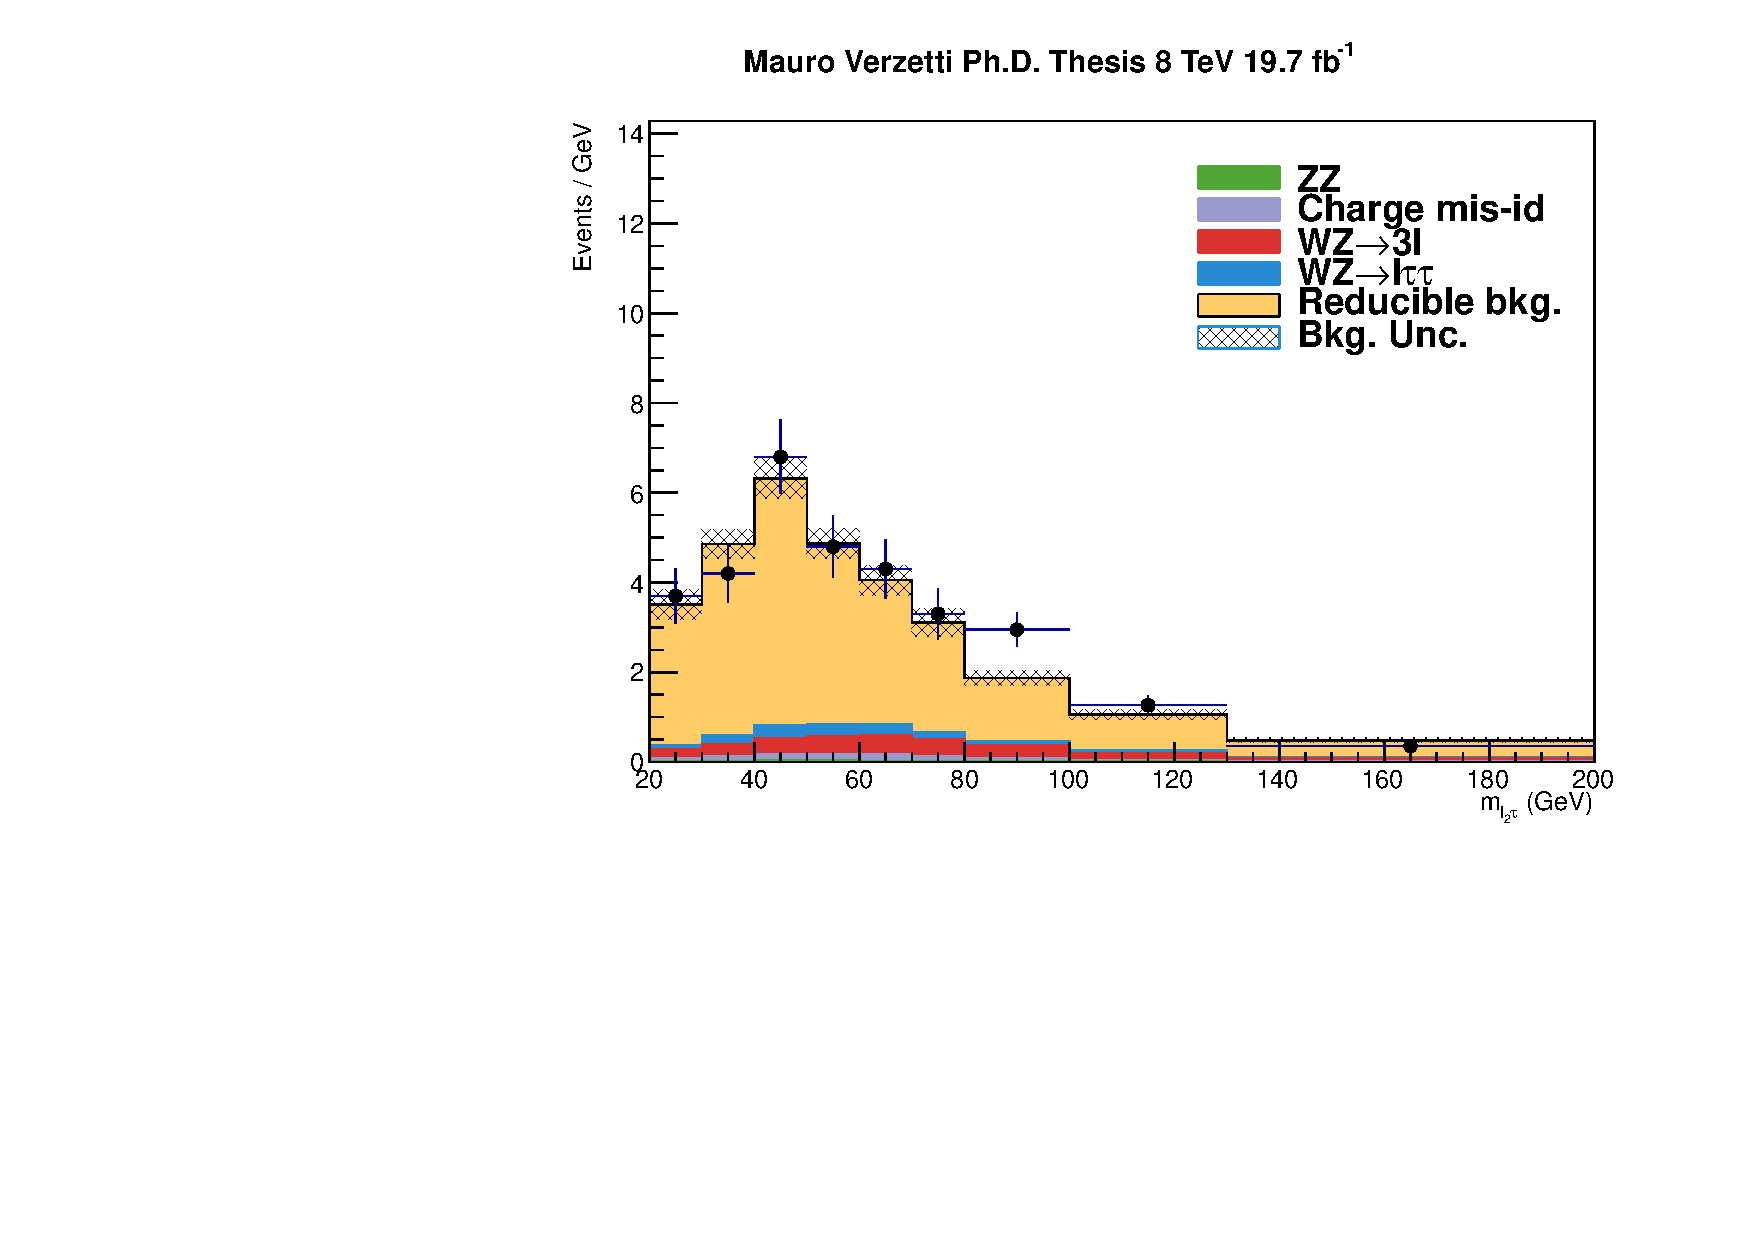
\includegraphics[width=0.49\textwidth]{4_Analisys/pics/8TeV/plots/emt/f3/Full/final-f3-subMass-Full.pdf}
  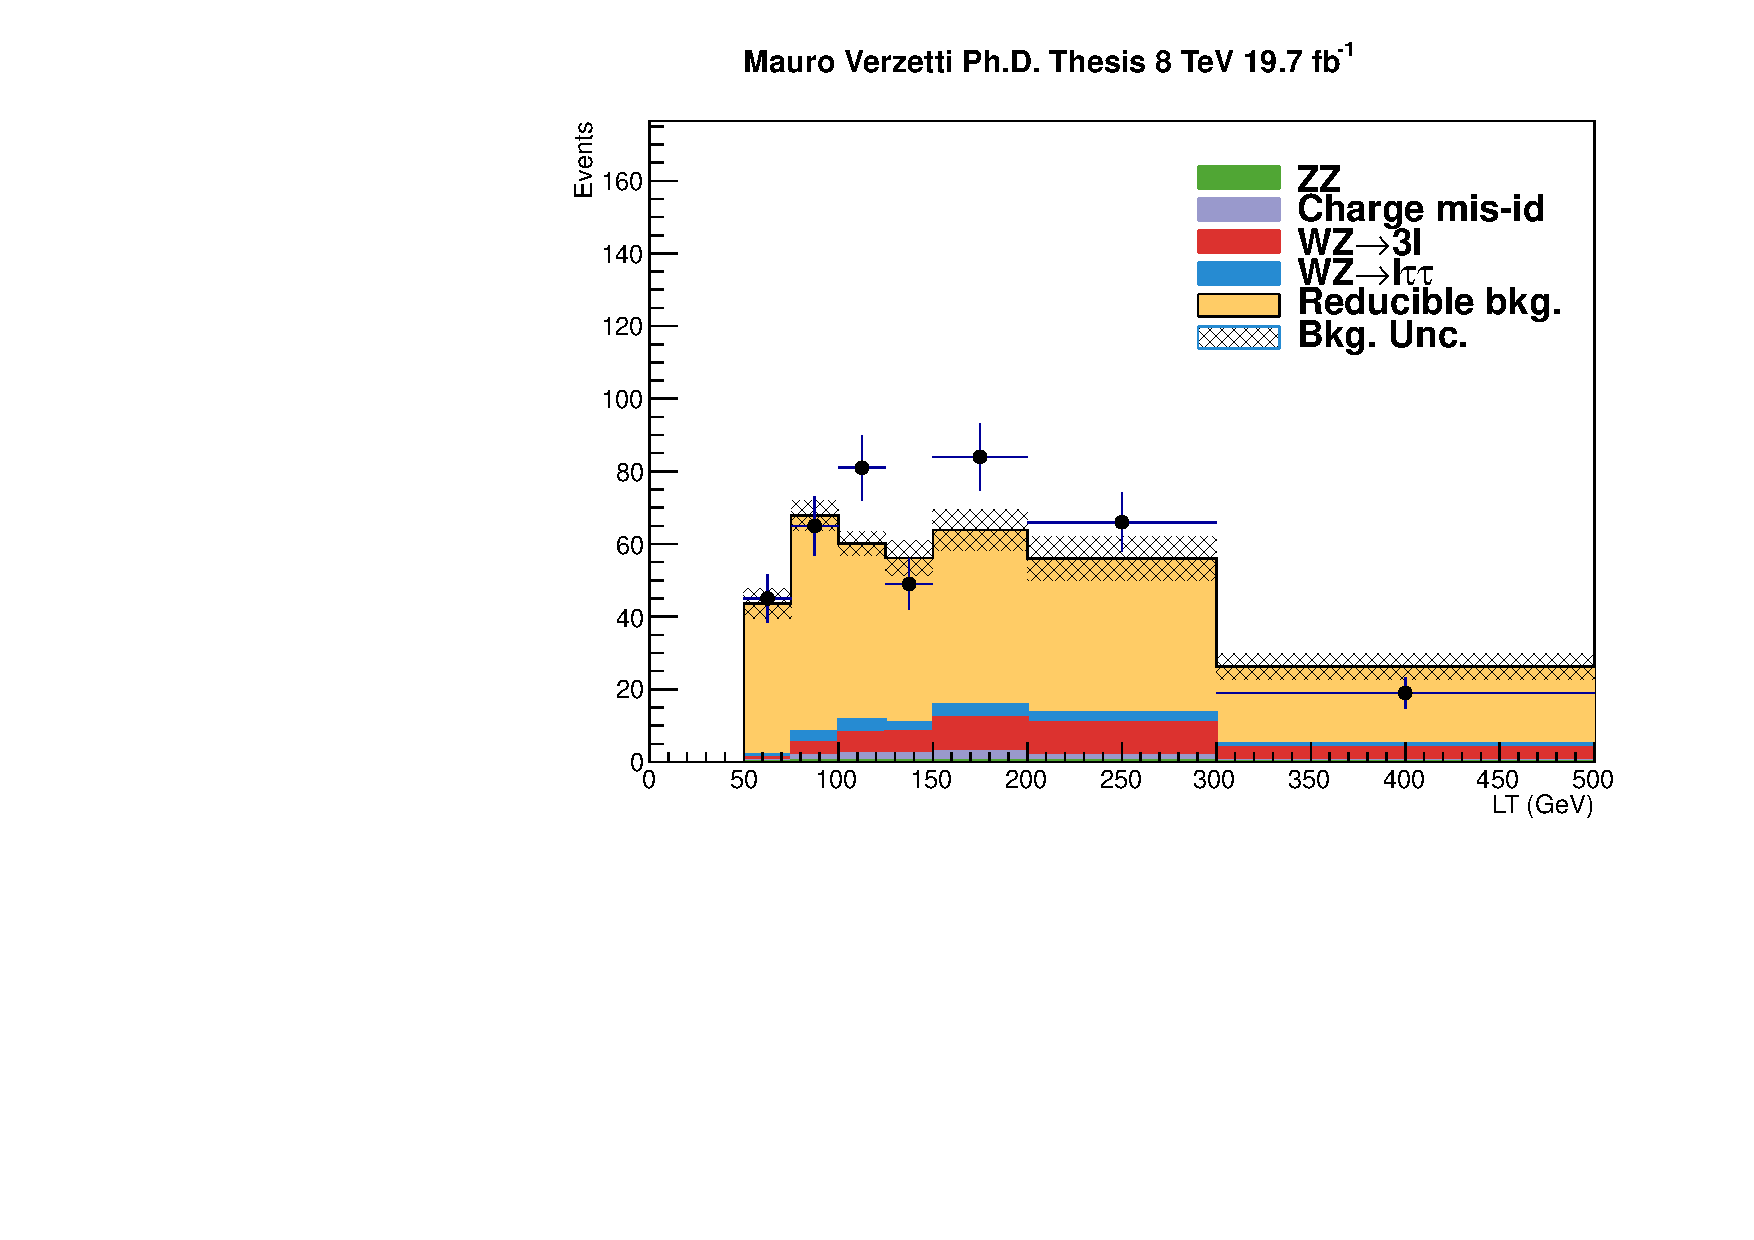
\includegraphics[width=0.49\textwidth]{4_Analisys/pics/8TeV/plots/emt/f3/final-f3-LT.pdf}\\
  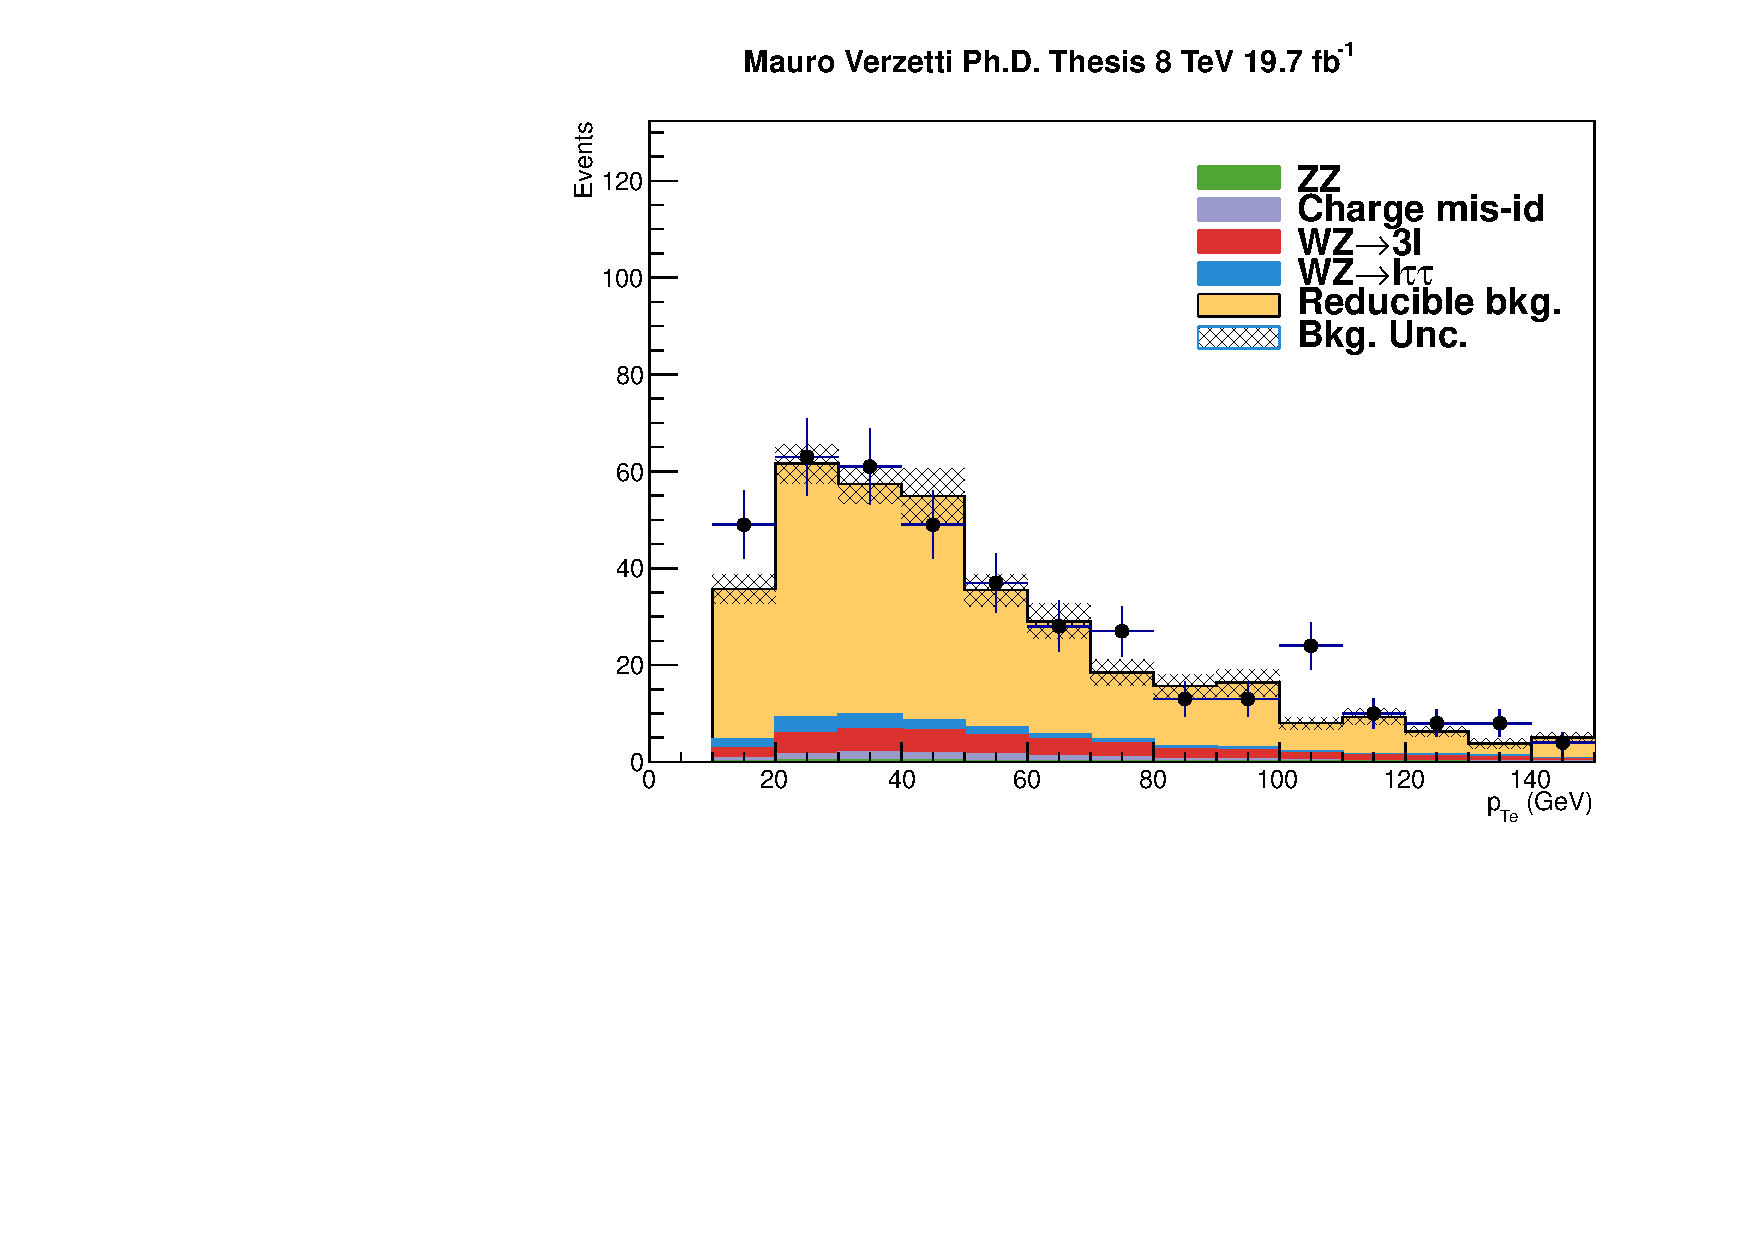
\includegraphics[width=0.49\textwidth]{4_Analisys/pics/8TeV/plots/emt/f3/Full/final-f3-ePt-Full.pdf}
  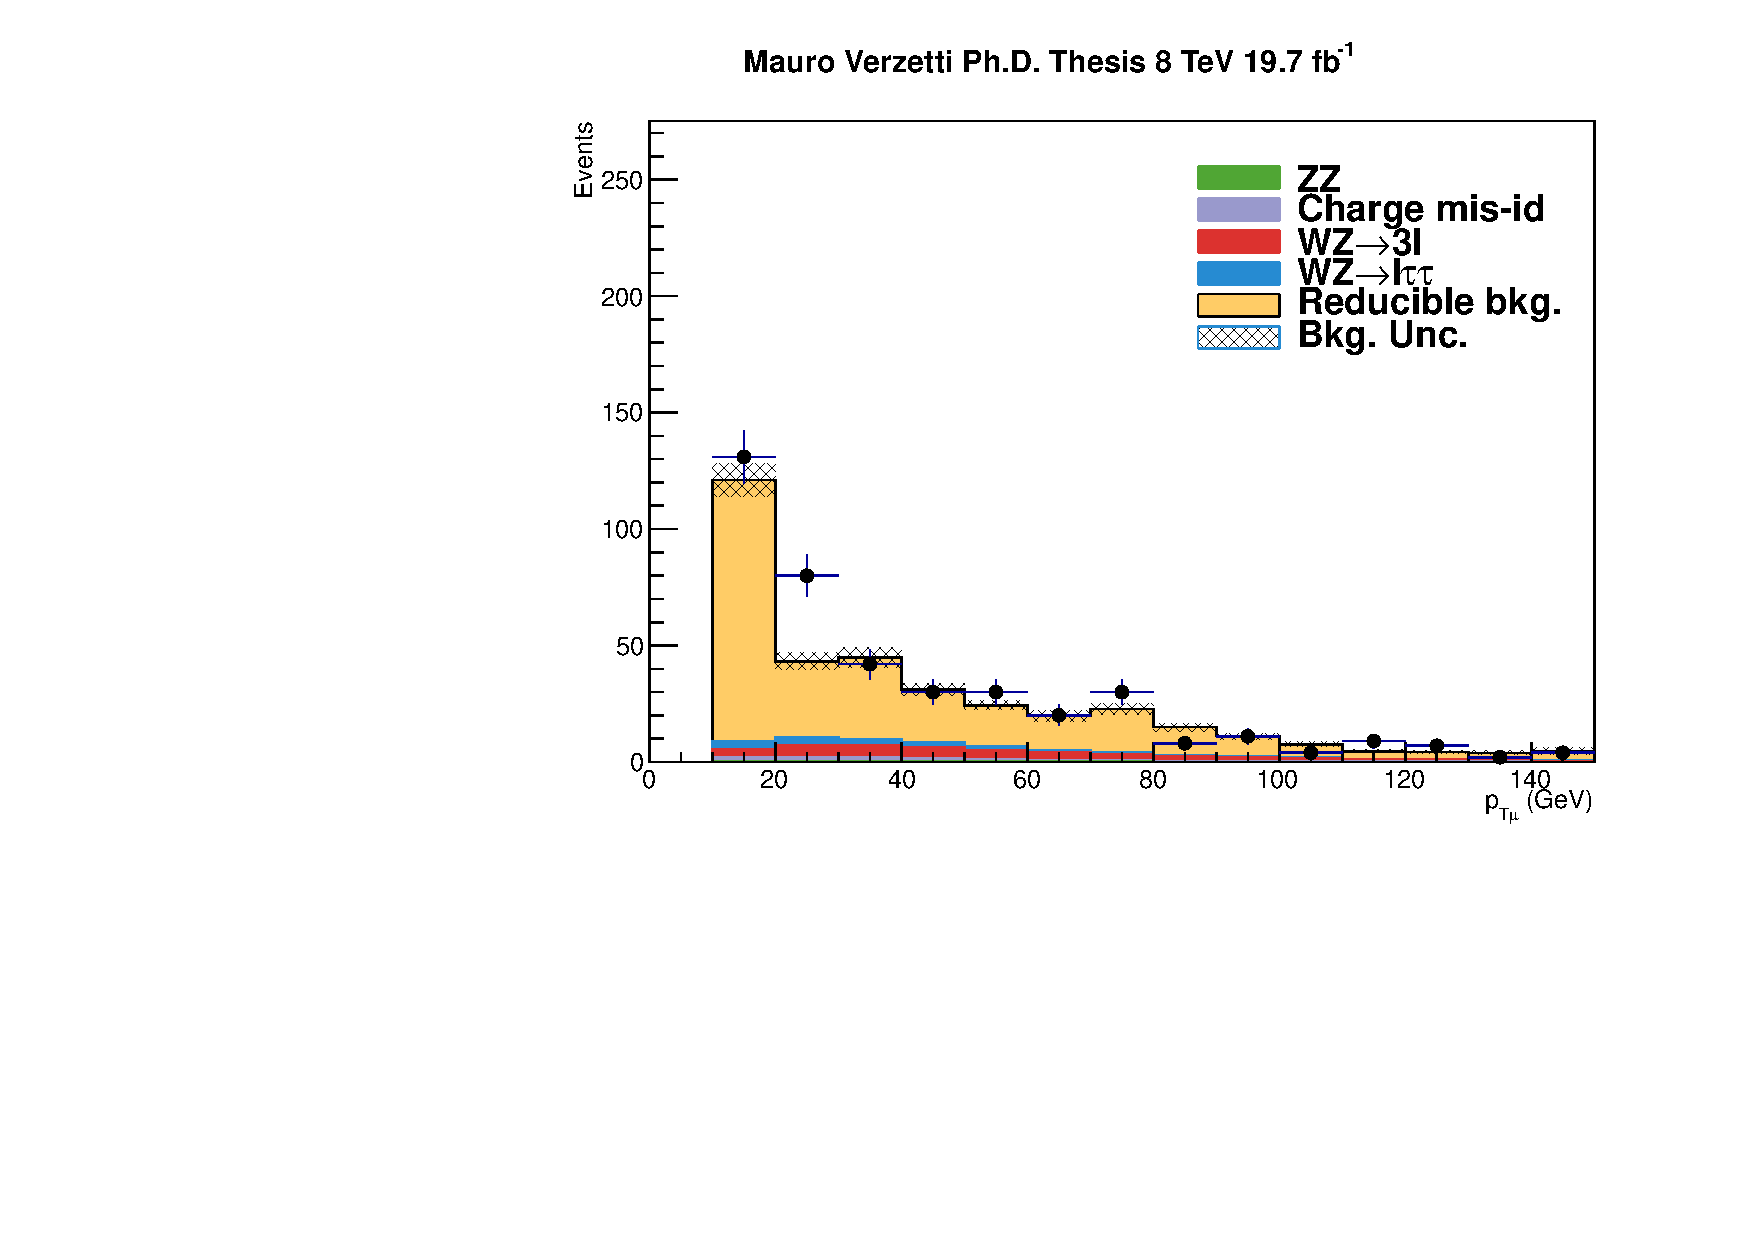
\includegraphics[width=0.49\textwidth]{4_Analisys/pics/8TeV/plots/emt/f3/Full/final-f3-mPt-Full.pdf}\\
  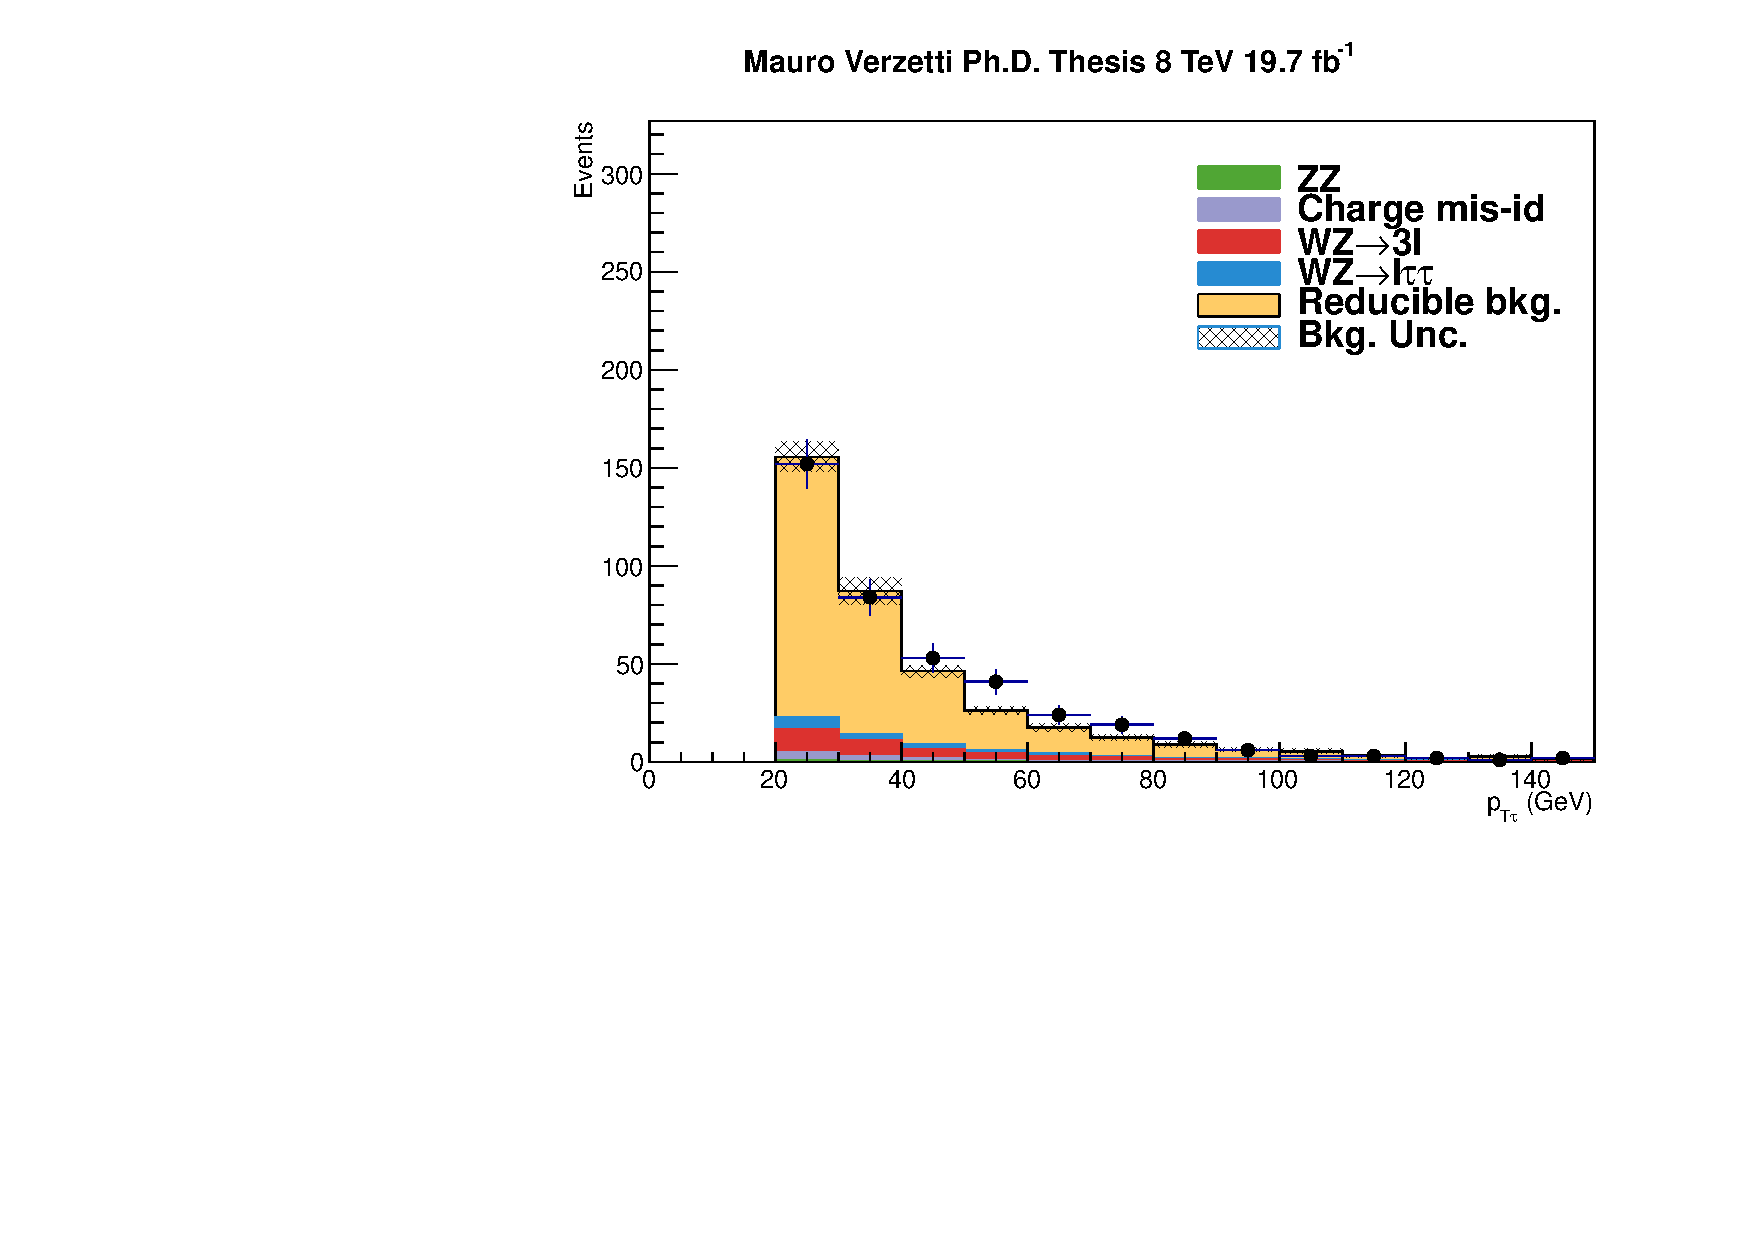
\includegraphics[width=0.49\textwidth]{4_Analisys/pics/8TeV/plots/emt/f3/Full/final-f3-tPt-Full.pdf}
  \caption{Comparison of measured and predicted backgrounds in the $e\mu\tau_h$ ``fake tau'' control region for 8 TeV data.
  From top left to bottom: mass of the sub-leading lepton and the tau system, scalar sum of the leptons \pT ($L_T$), \pT of the electron, muon, and hadronic tau.
  The non-prompt background estimate is computed in the same manner as that in the signal region.
  The shaded band represents the background uncertainty.
  }
  \label{fig:LLT_emt_f3_control_8TeV}
\end{center}
\end{figure}


\begin{figure}
\begin{center}
  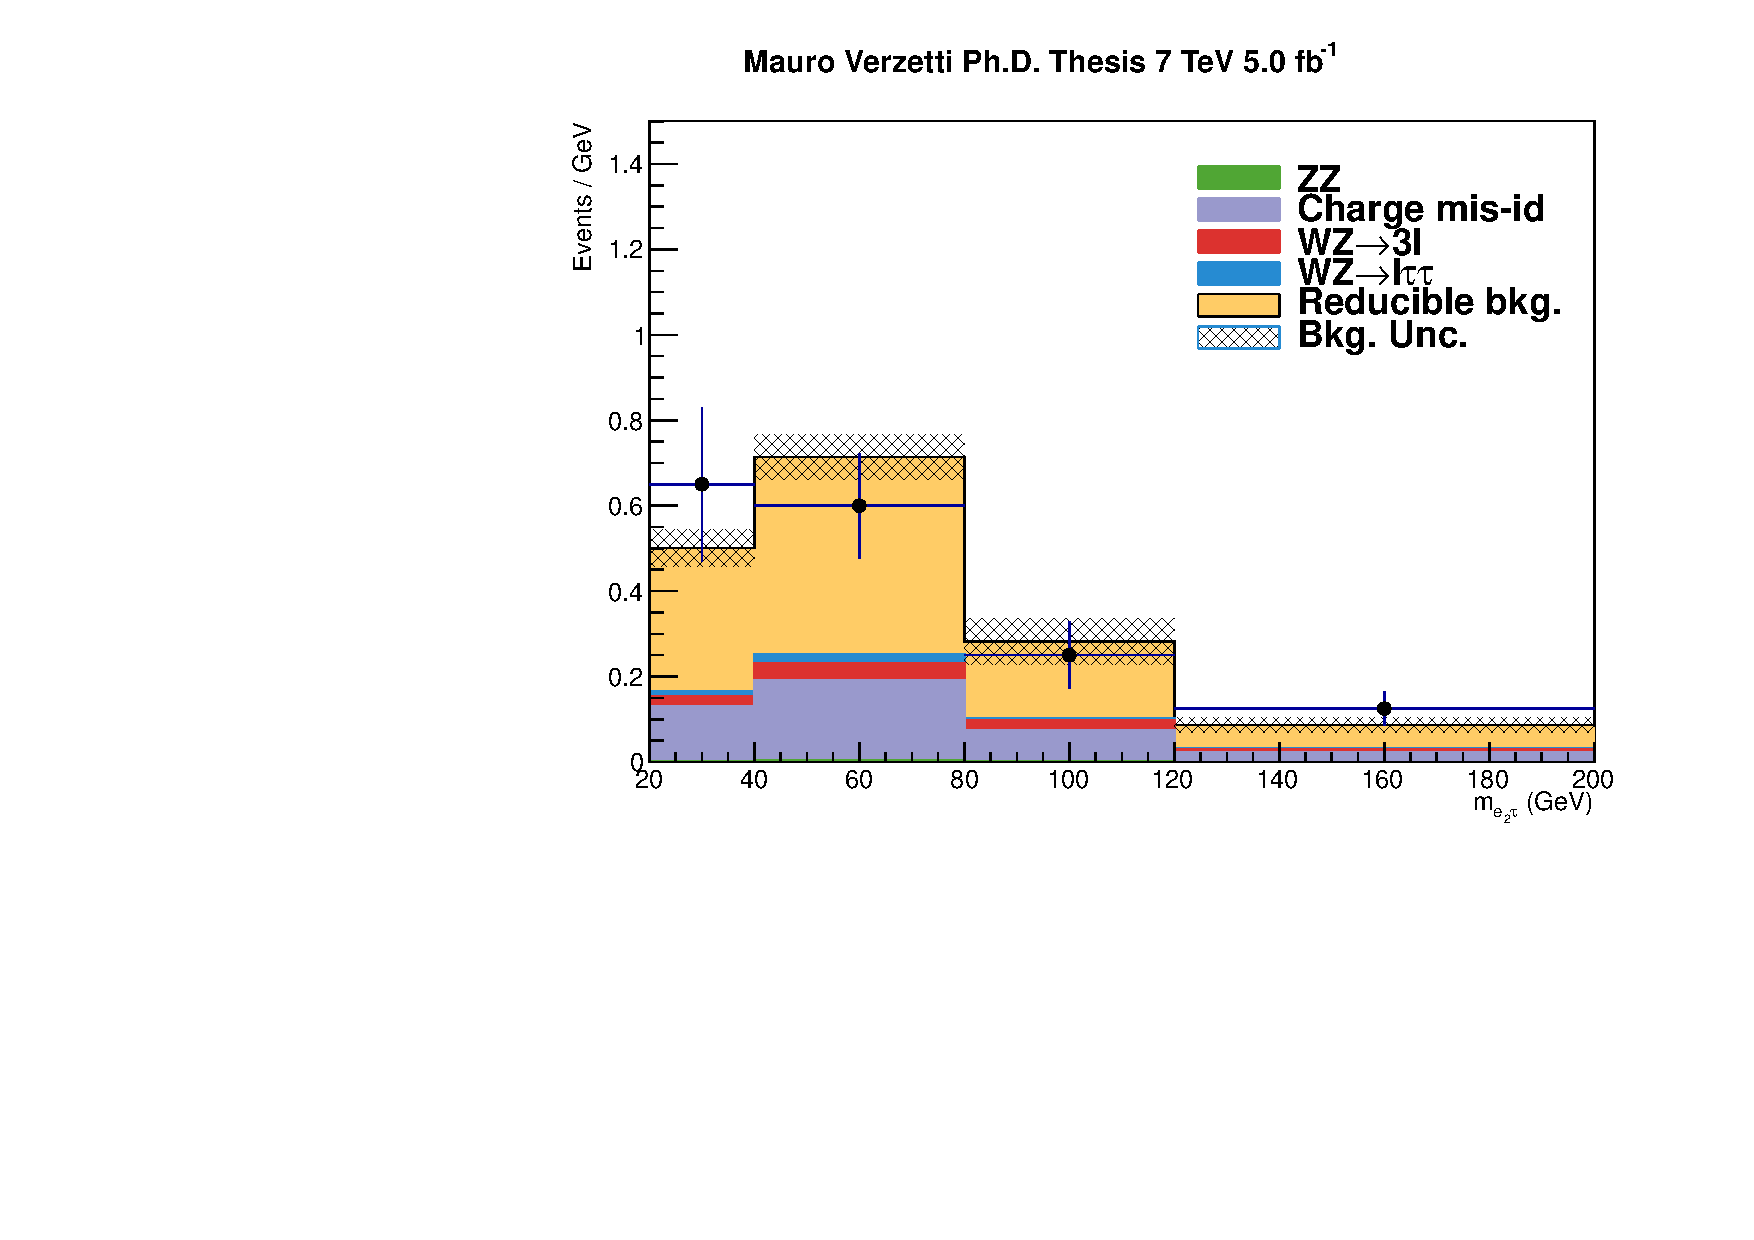
\includegraphics[width=0.49\textwidth]{4_Analisys/pics/7TeV/plots/eet/f3/Full/final-f3-subMass-Full.pdf}
  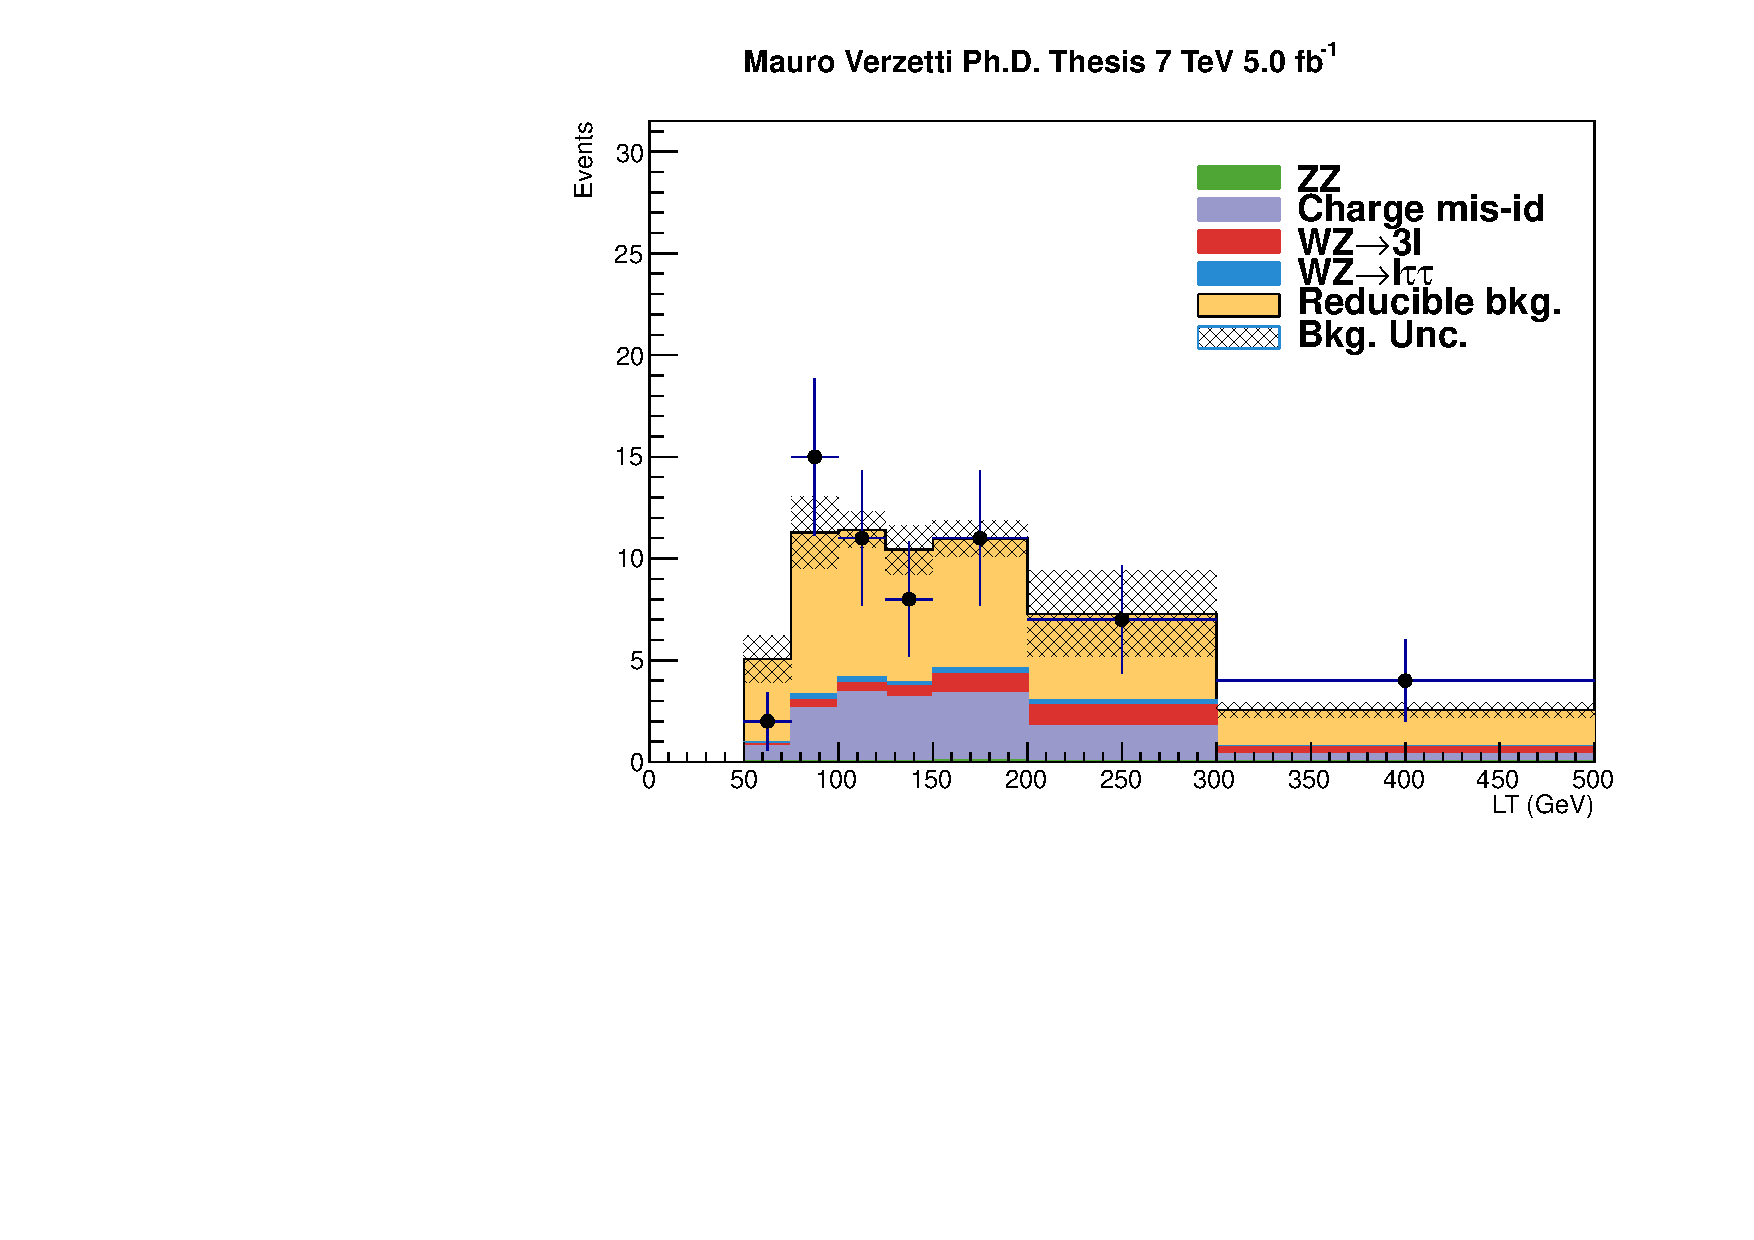
\includegraphics[width=0.49\textwidth]{4_Analisys/pics/7TeV/plots/eet/f3/final-f3-LT.pdf}\\
  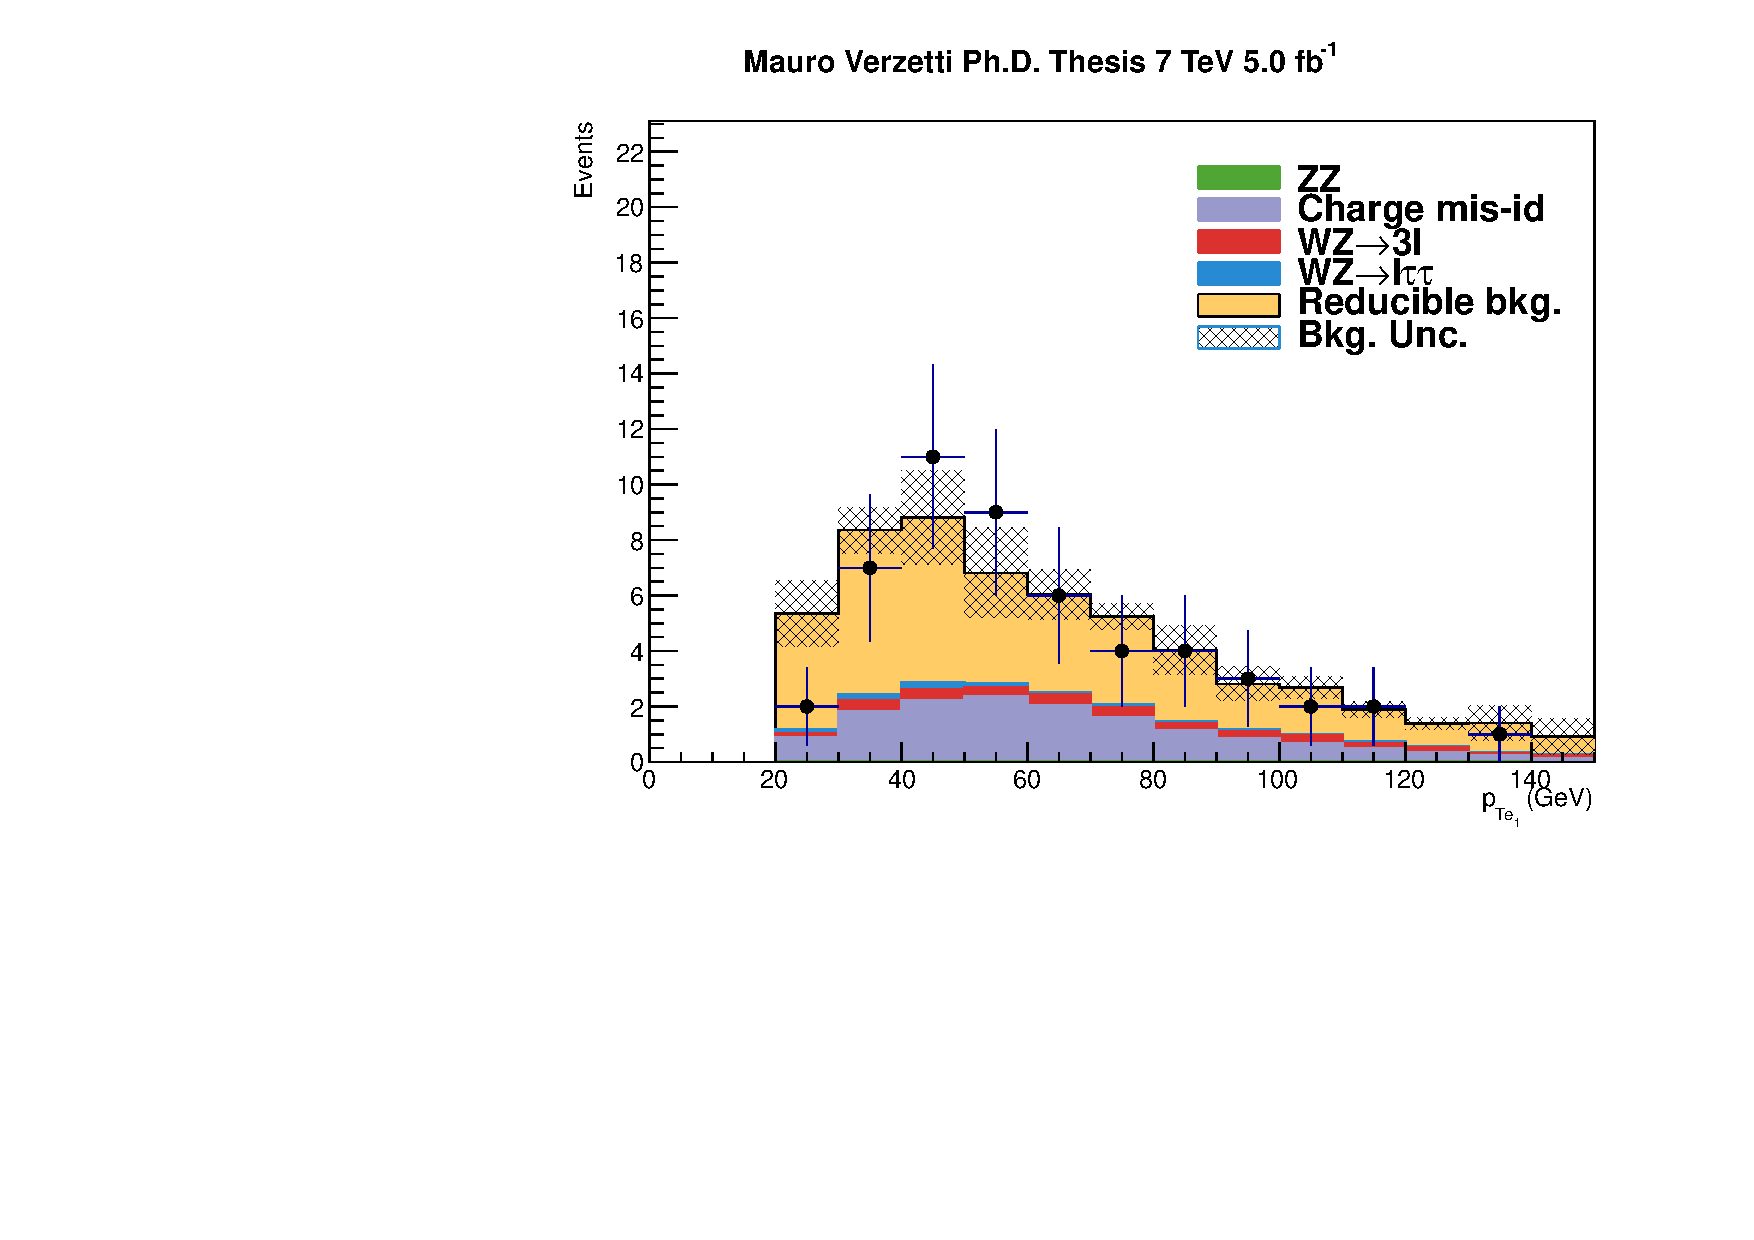
\includegraphics[width=0.49\textwidth]{4_Analisys/pics/7TeV/plots/eet/f3/Full/final-f3-e1Pt-Full.pdf}
  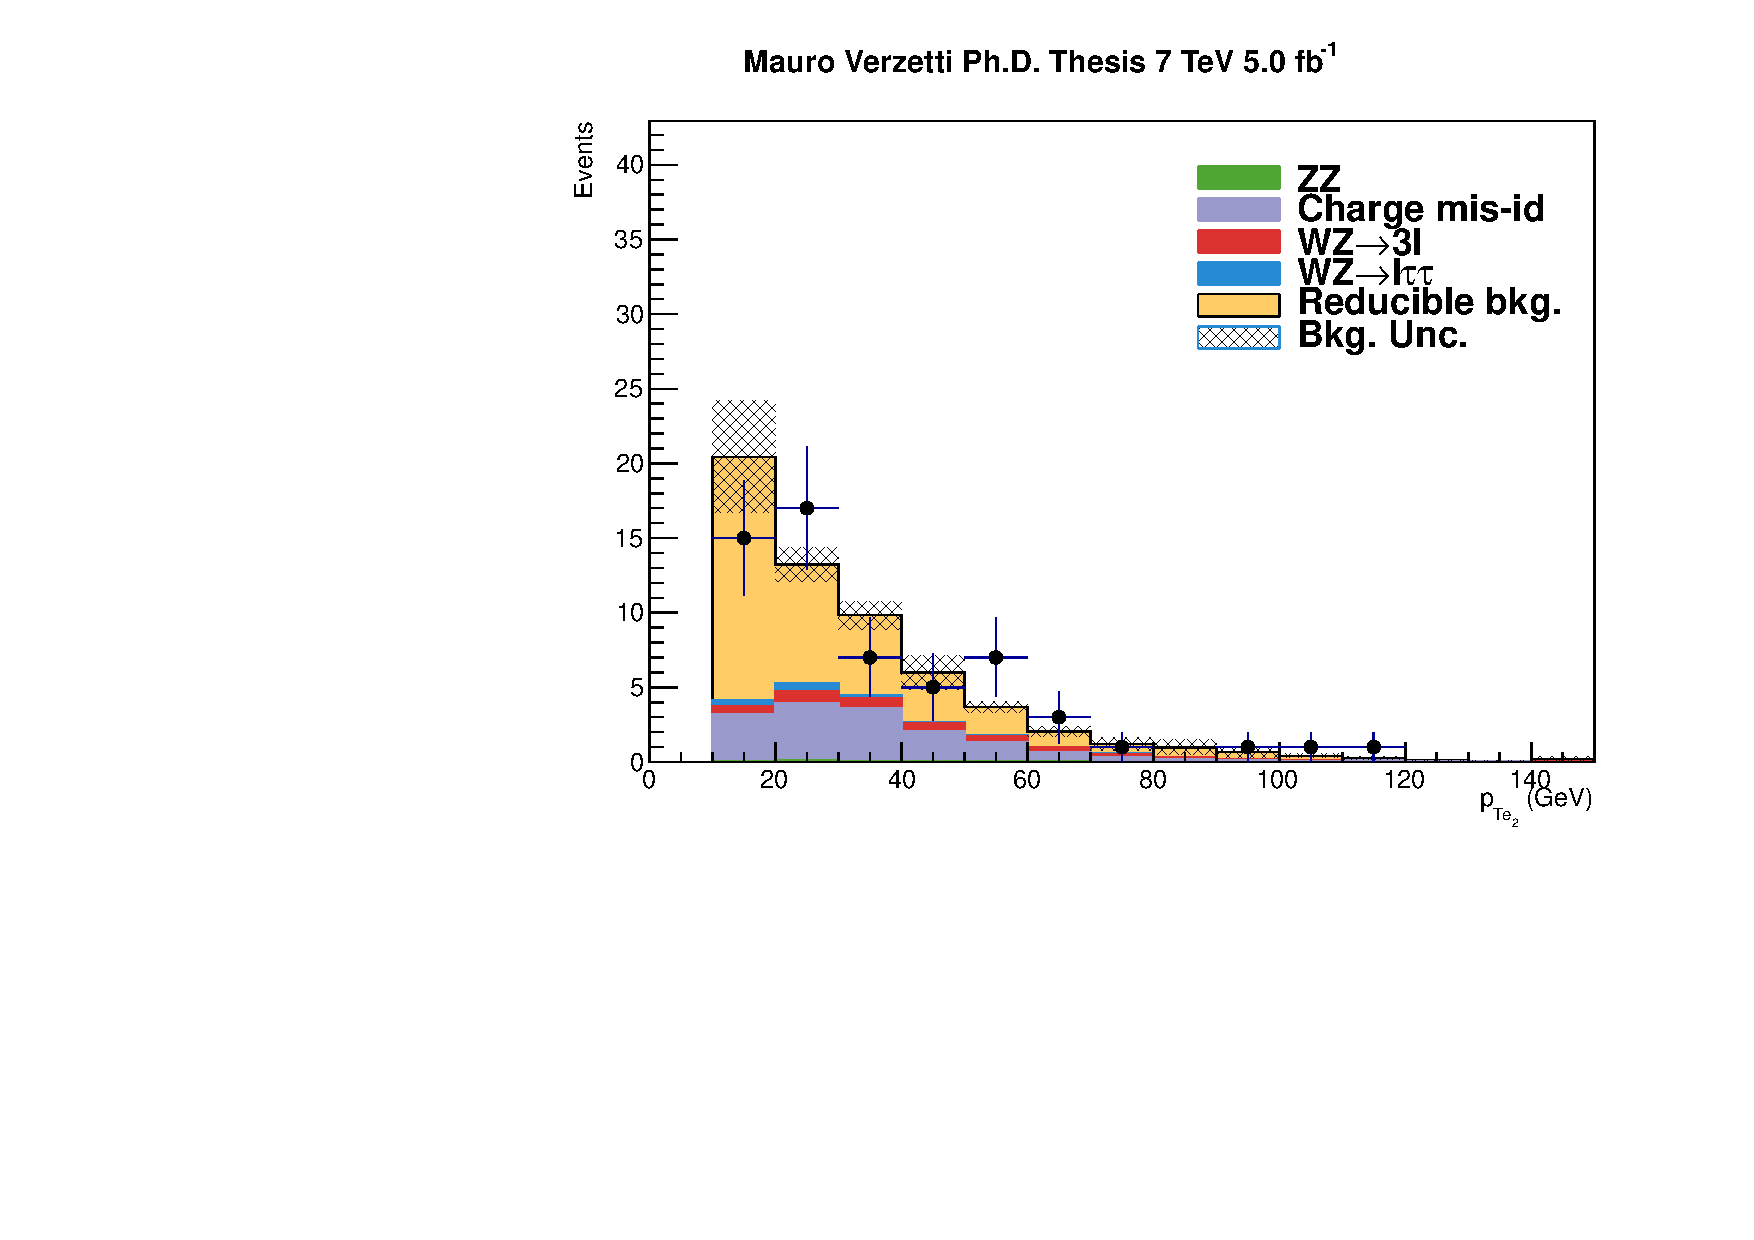
\includegraphics[width=0.49\textwidth]{4_Analisys/pics/7TeV/plots/eet/f3/Full/final-f3-e2Pt-Full.pdf}\\
  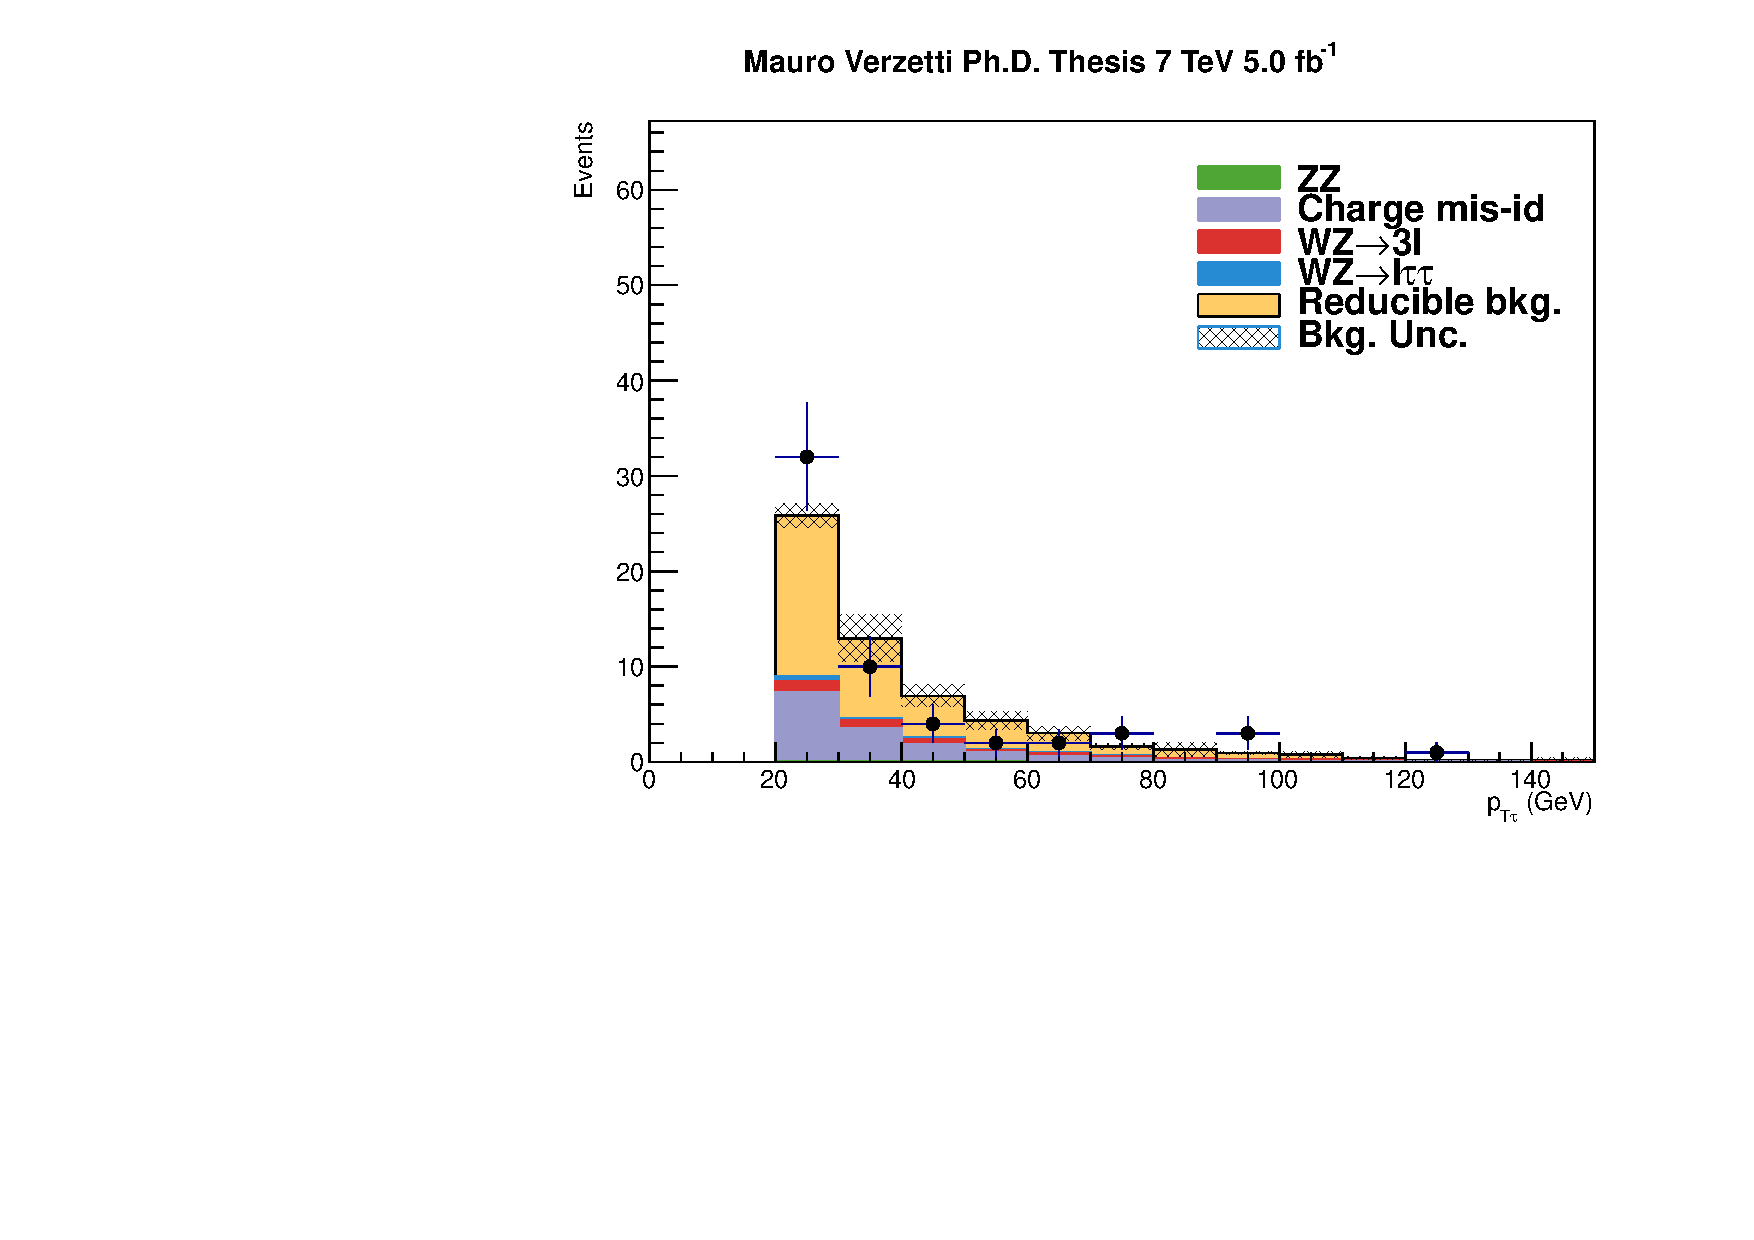
\includegraphics[width=0.49\textwidth]{4_Analisys/pics/7TeV/plots/eet/f3/Full/final-f3-tPt-Full.pdf}
  \caption{Comparison of measured and predicted backgrounds in the $ee\tau_h$ ``fake tau'' control region for 7 TeV data.
  From top left to bottom: mass of the sub-leading electron and the tau system, scalar sum of the leptons \pT ($L_T$), \pT of the leading and sub-leading electron, and \pT of the hadronic tau.
  The non-prompt background estimate is computed in the same manner as that in the signal region.
  The shaded band represents the background uncertainty.
  }
  \label{fig:LLT_eet_f3_control_7TeV}
\end{center}
\end{figure}

\begin{figure}
\begin{center}
  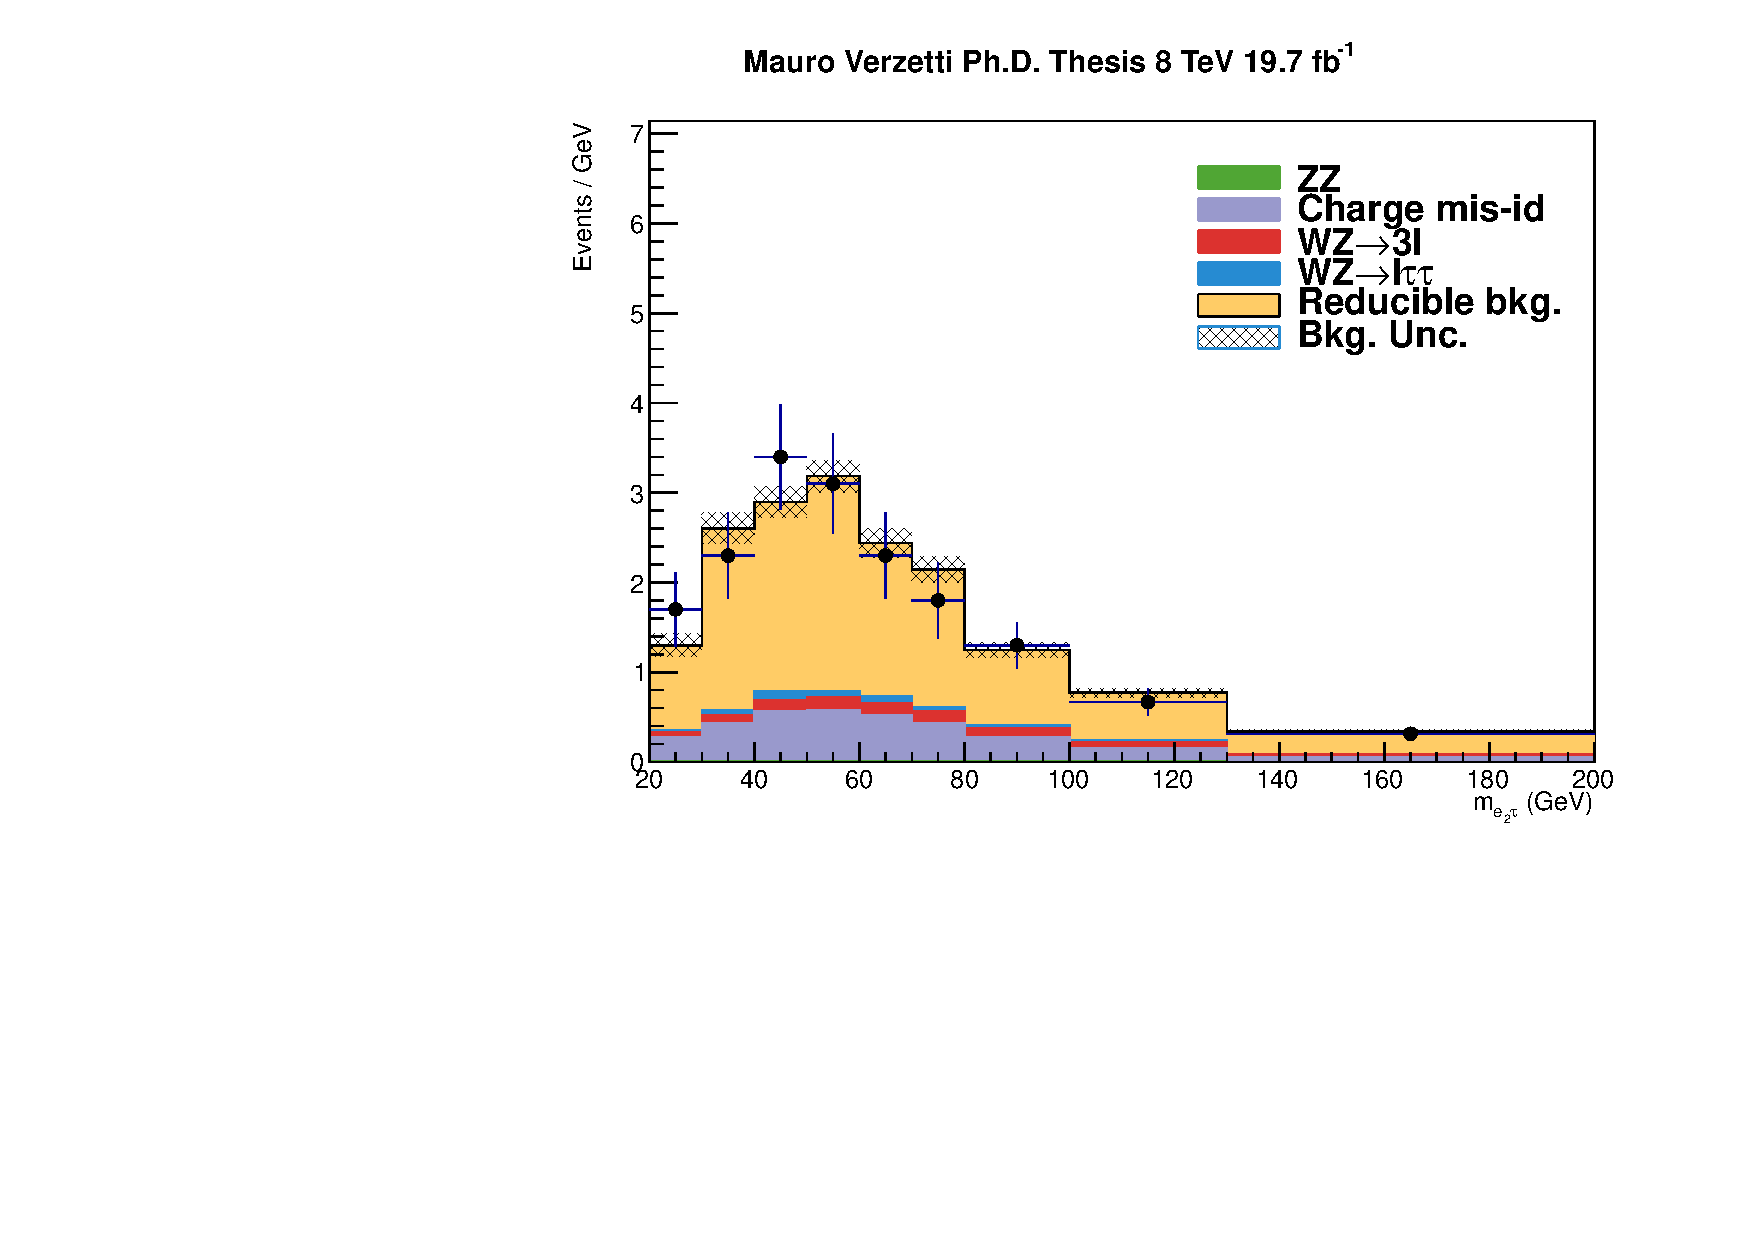
\includegraphics[width=0.49\textwidth]{4_Analisys/pics/8TeV/plots/eet/f3/Full/final-f3-subMass-Full.pdf}
  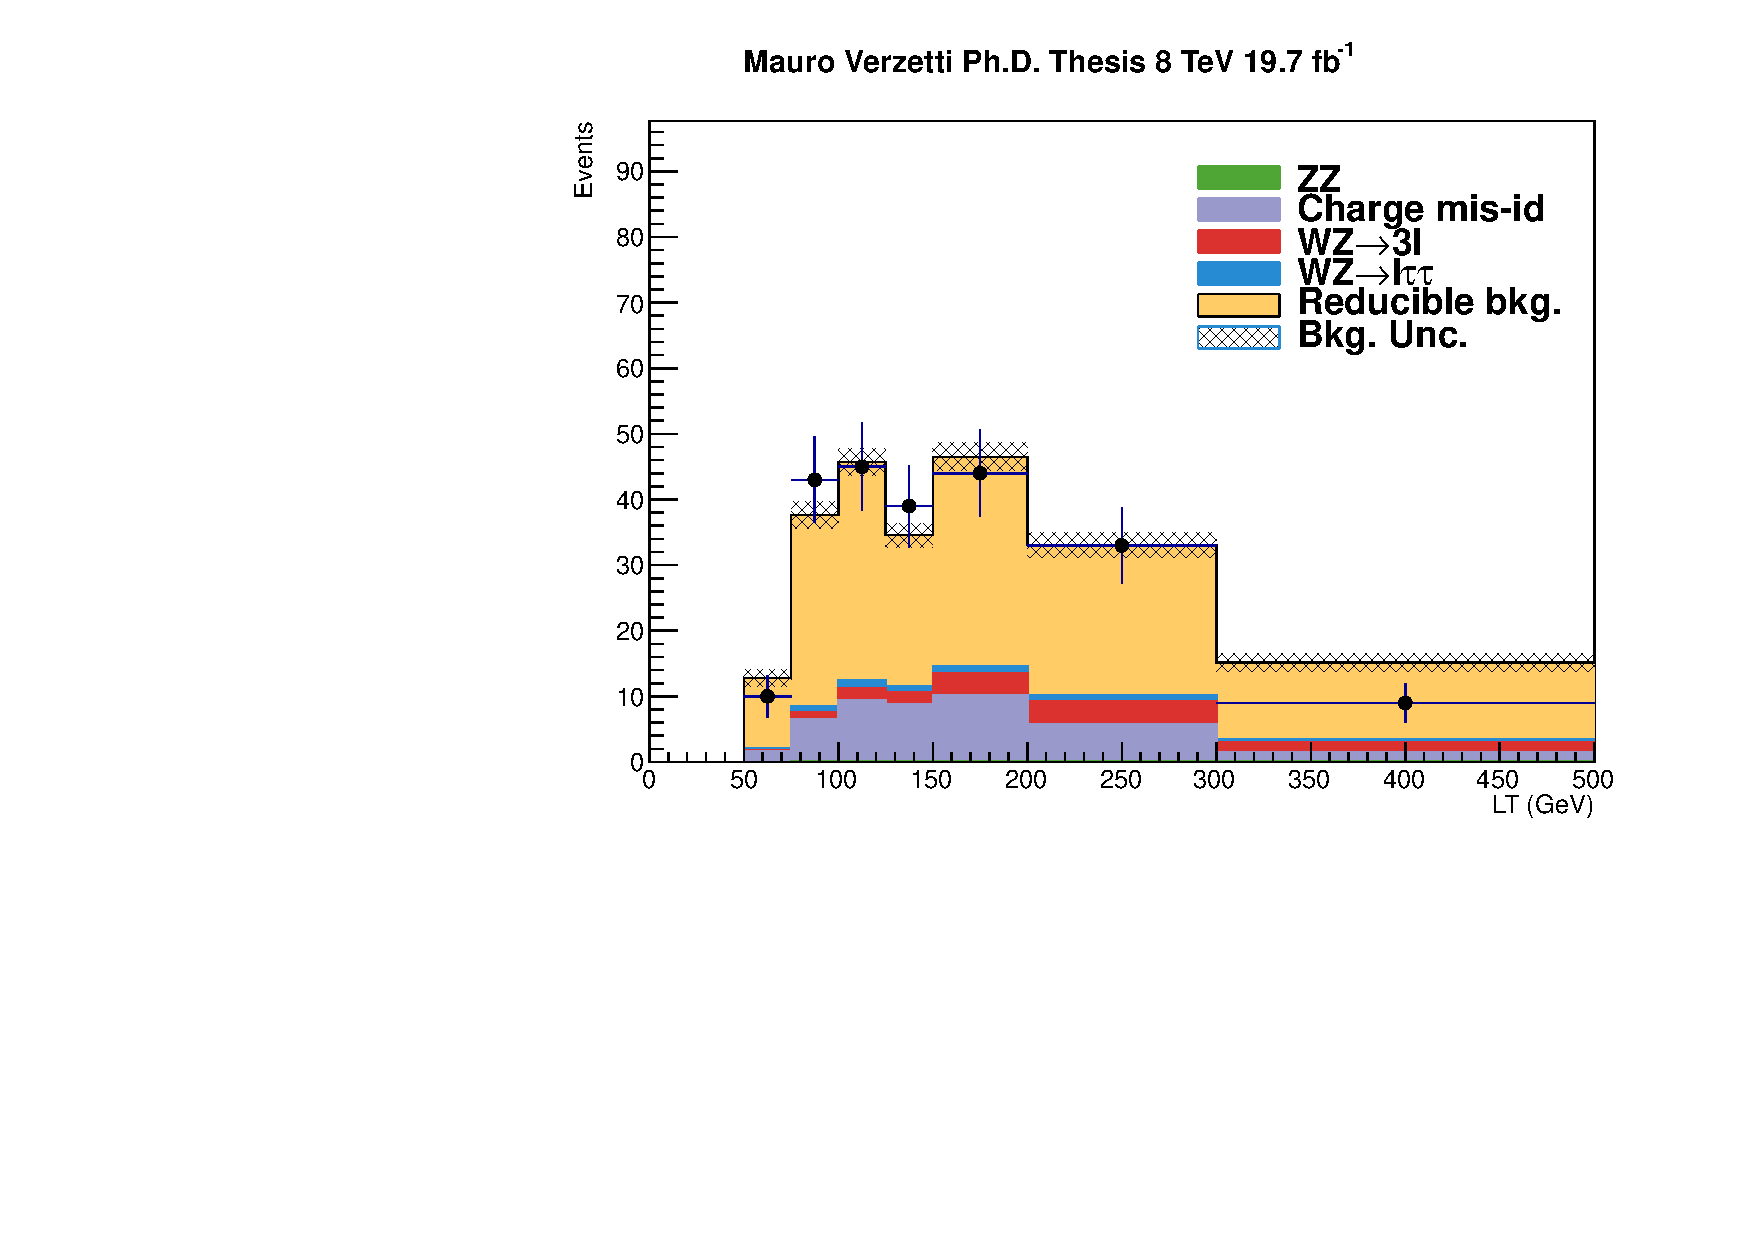
\includegraphics[width=0.49\textwidth]{4_Analisys/pics/8TeV/plots/eet/f3/final-f3-LT.pdf}\\
  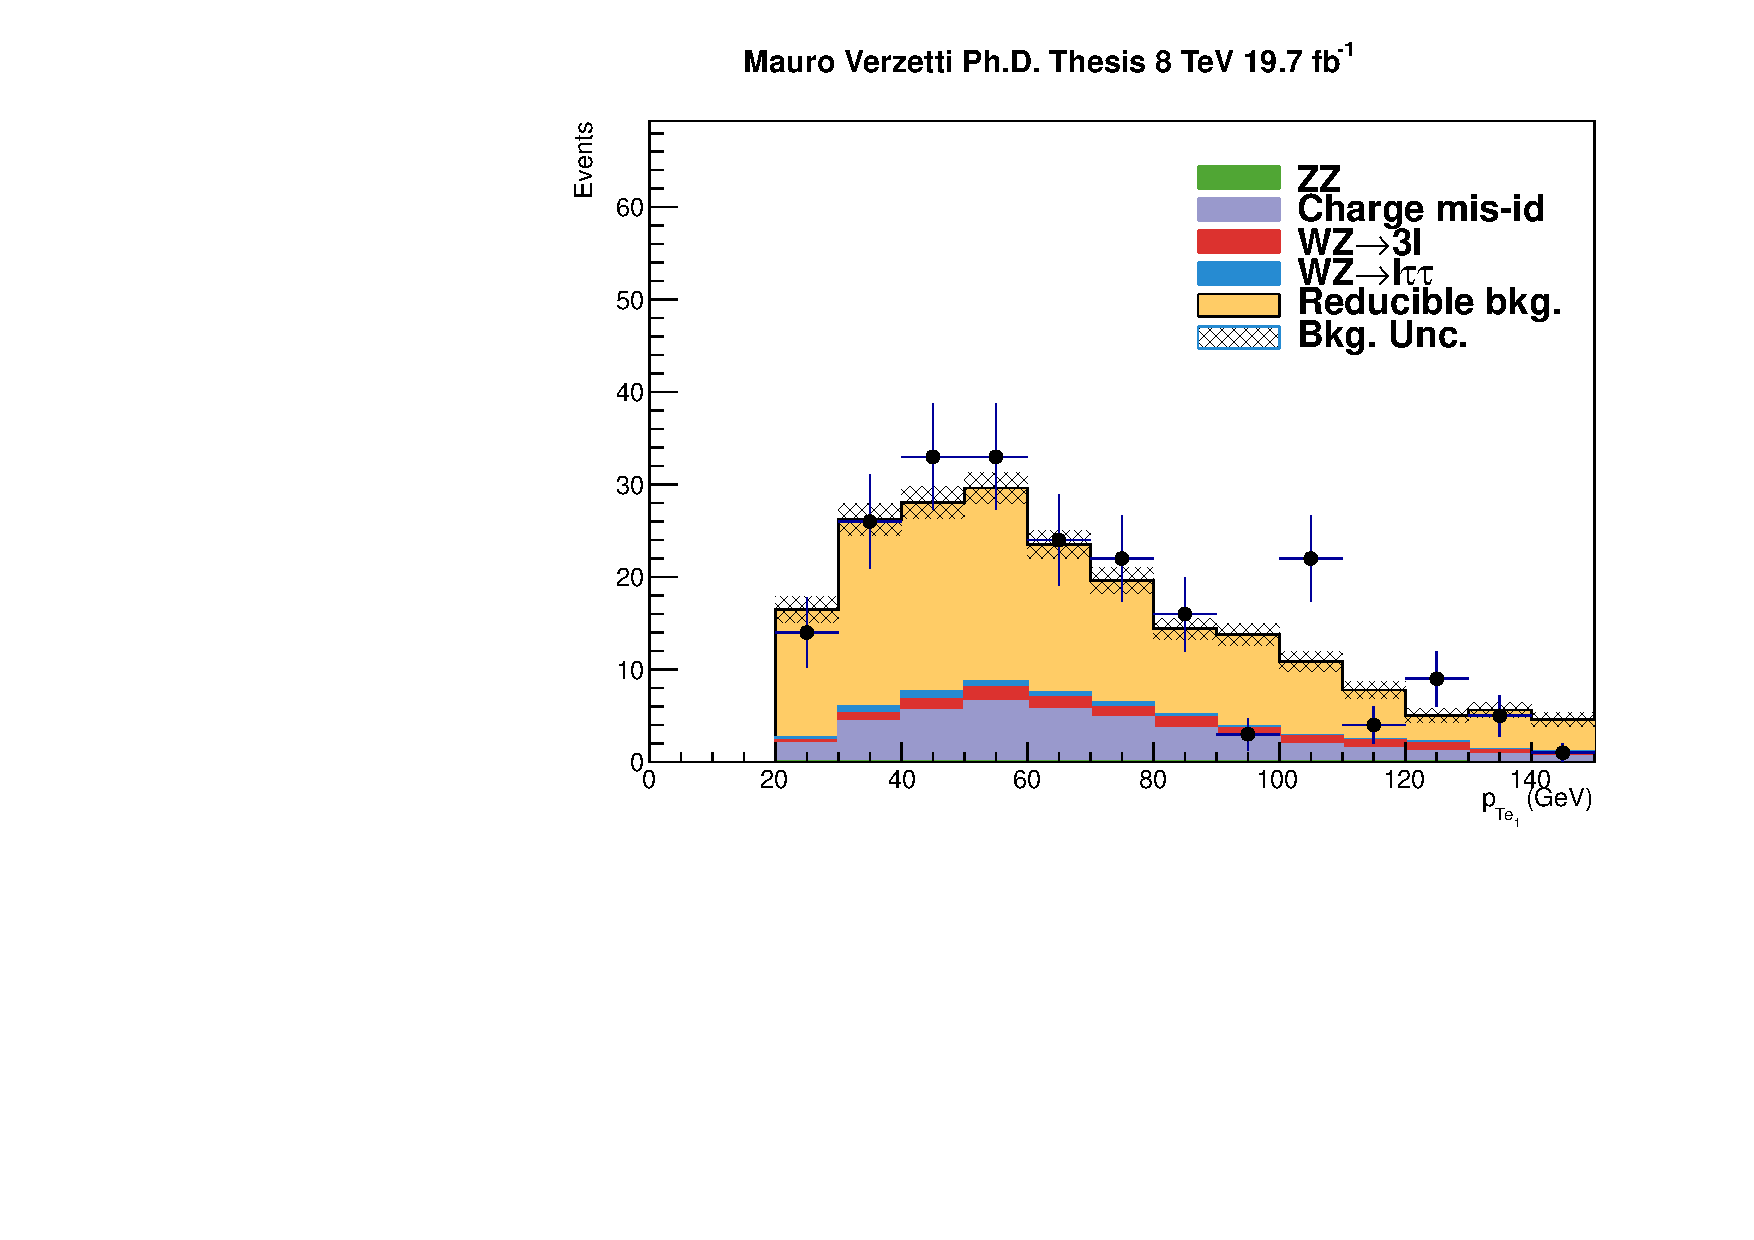
\includegraphics[width=0.49\textwidth]{4_Analisys/pics/8TeV/plots/eet/f3/Full/final-f3-e1Pt-Full.pdf}
  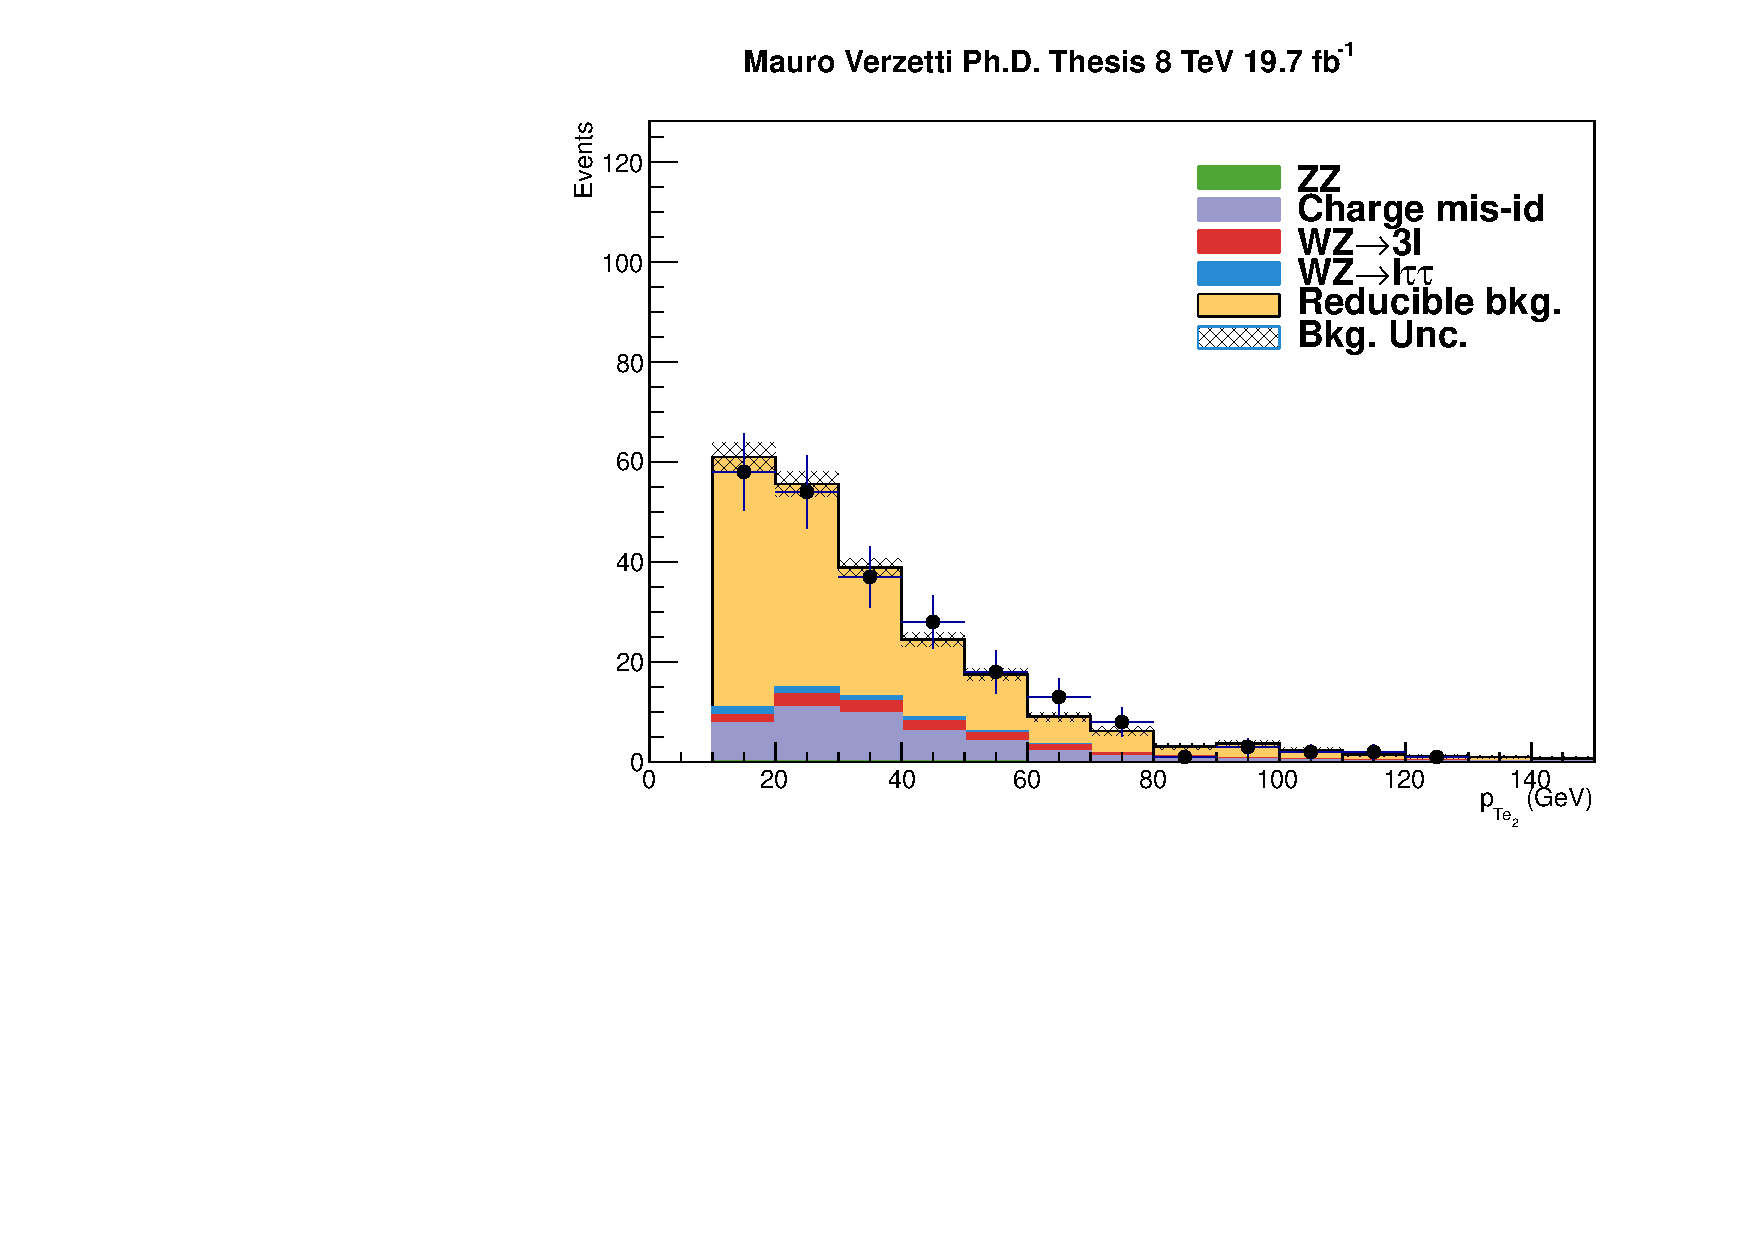
\includegraphics[width=0.49\textwidth]{4_Analisys/pics/8TeV/plots/eet/f3/Full/final-f3-e2Pt-Full.pdf}\\
  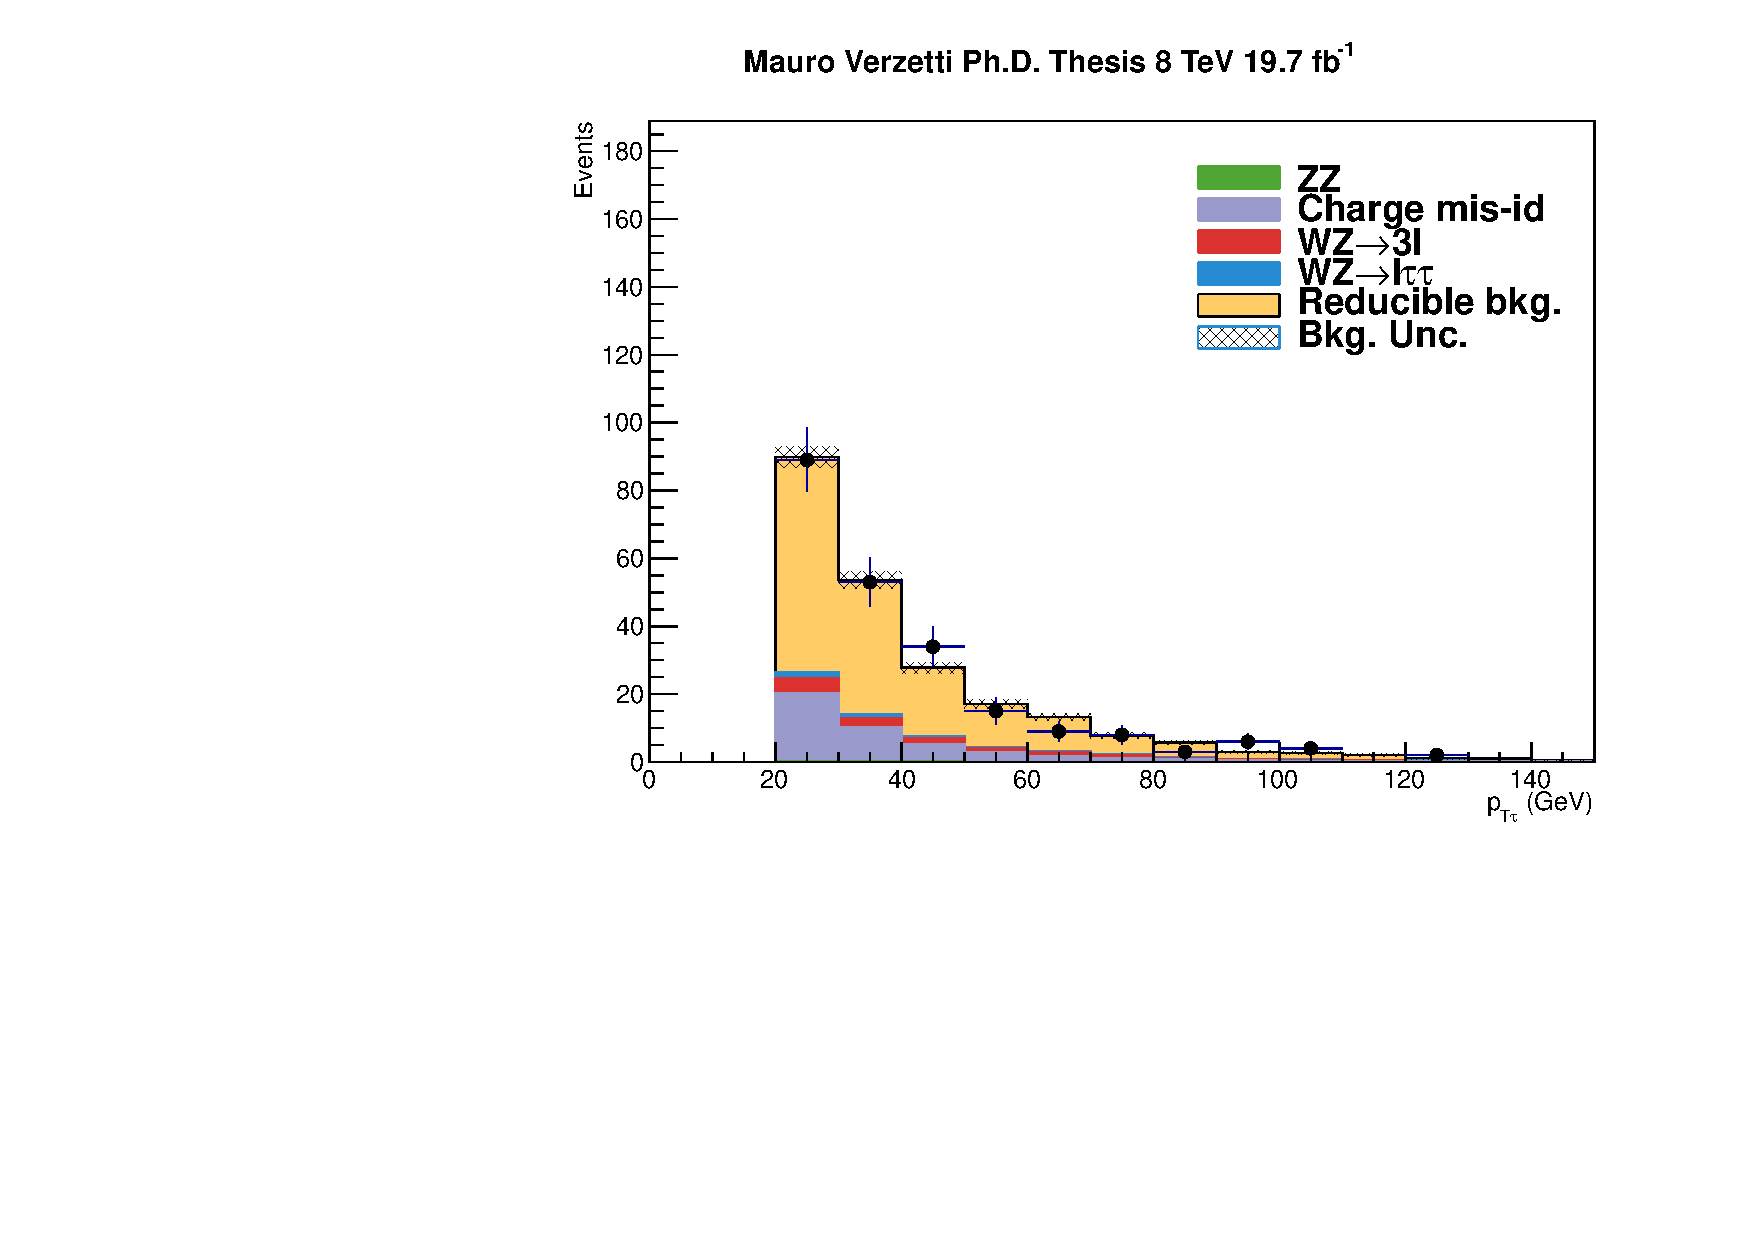
\includegraphics[width=0.49\textwidth]{4_Analisys/pics/8TeV/plots/eet/f3/Full/final-f3-tPt-Full.pdf}
  \caption{Comparison of measured and predicted backgrounds in the $ee\tau_h$ ``fake tau'' control region for 8 TeV data.
  From top left to bottom: mass of the sub-leading electron and the tau system, scalar sum of the leptons \pT ($L_T$), \pT of the leading and sub-leading electron, and \pT of the hadronic tau.
  The non-prompt background estimate is computed in the same manner as that in the signal region.
  The shaded band represents the background uncertainty.
  }
  \label{fig:LLT_eet_f3_control_8TeV}
\end{center}
\end{figure}

\subsection{Fake tau method}

To better estimate the solidity of the the ``fake lepton'' method against differences in composition of the training sample and the sample to which the method is applied, a second background estimate is performed.
This methodology is very similar to the previous one, but the object considered as possibly mis-reconstructed is the hadronic tau.

\subsubsection{Region definition}

The misidentification probability for $\tau_h$ candidates is measured in $W+$Jets events, requiring:
\begin{itemize}
\item Events must pass the single muon trigger;
\item A muon candidate with $\pt > 24$ GeV and $|\eta| < 2.1$;
\item The muon must pass the tight Particle Flow identification and have a combined PF Relative Isolation $\Delta \beta $ corrected below $0.1$;
\item The longitudinal impact parameter of the lepton track with respect to the primary vertex must be less than 0.2 cm;
\item $m_{T}(\mu, \met) > 40\GeV$;
\item Two same sign tau candidates are required, both with opposite charge to the muon;
\item Events are rejected if they contain another muon or electron with $\pt > 15$ GeV;
\item Events are rejected if they contain a jet with $\pt > 20$ GeV and $|\eta|< 2.4$ satisfying the loose CSV b--tagging working point.
\end{itemize}
The tau fake-rate is measured individually for the 2011 and 2012 run periods in three regions of pseudo-rapidity ($|\eta|<0.8$,
\mbox{$0.8<|\eta|<1.6$} and $1.6<|\eta|<2.3$) and as a function of the tau \pT. The chosen fake-rate is modeled with a Landau with peak and
width left free to float.%, and an additive constant.

The measured tau misidentification rates in both 7 TeV and 8 TeV data are shown in Fig.~\ref{fig:LLT_tau_FR}. The measured tau misidentification rate spans from 6\% at low tau \pT in the end--cap region, to 1\% at high \pT ($ > 80$ GeV) in the central region.

\begin{figure}
  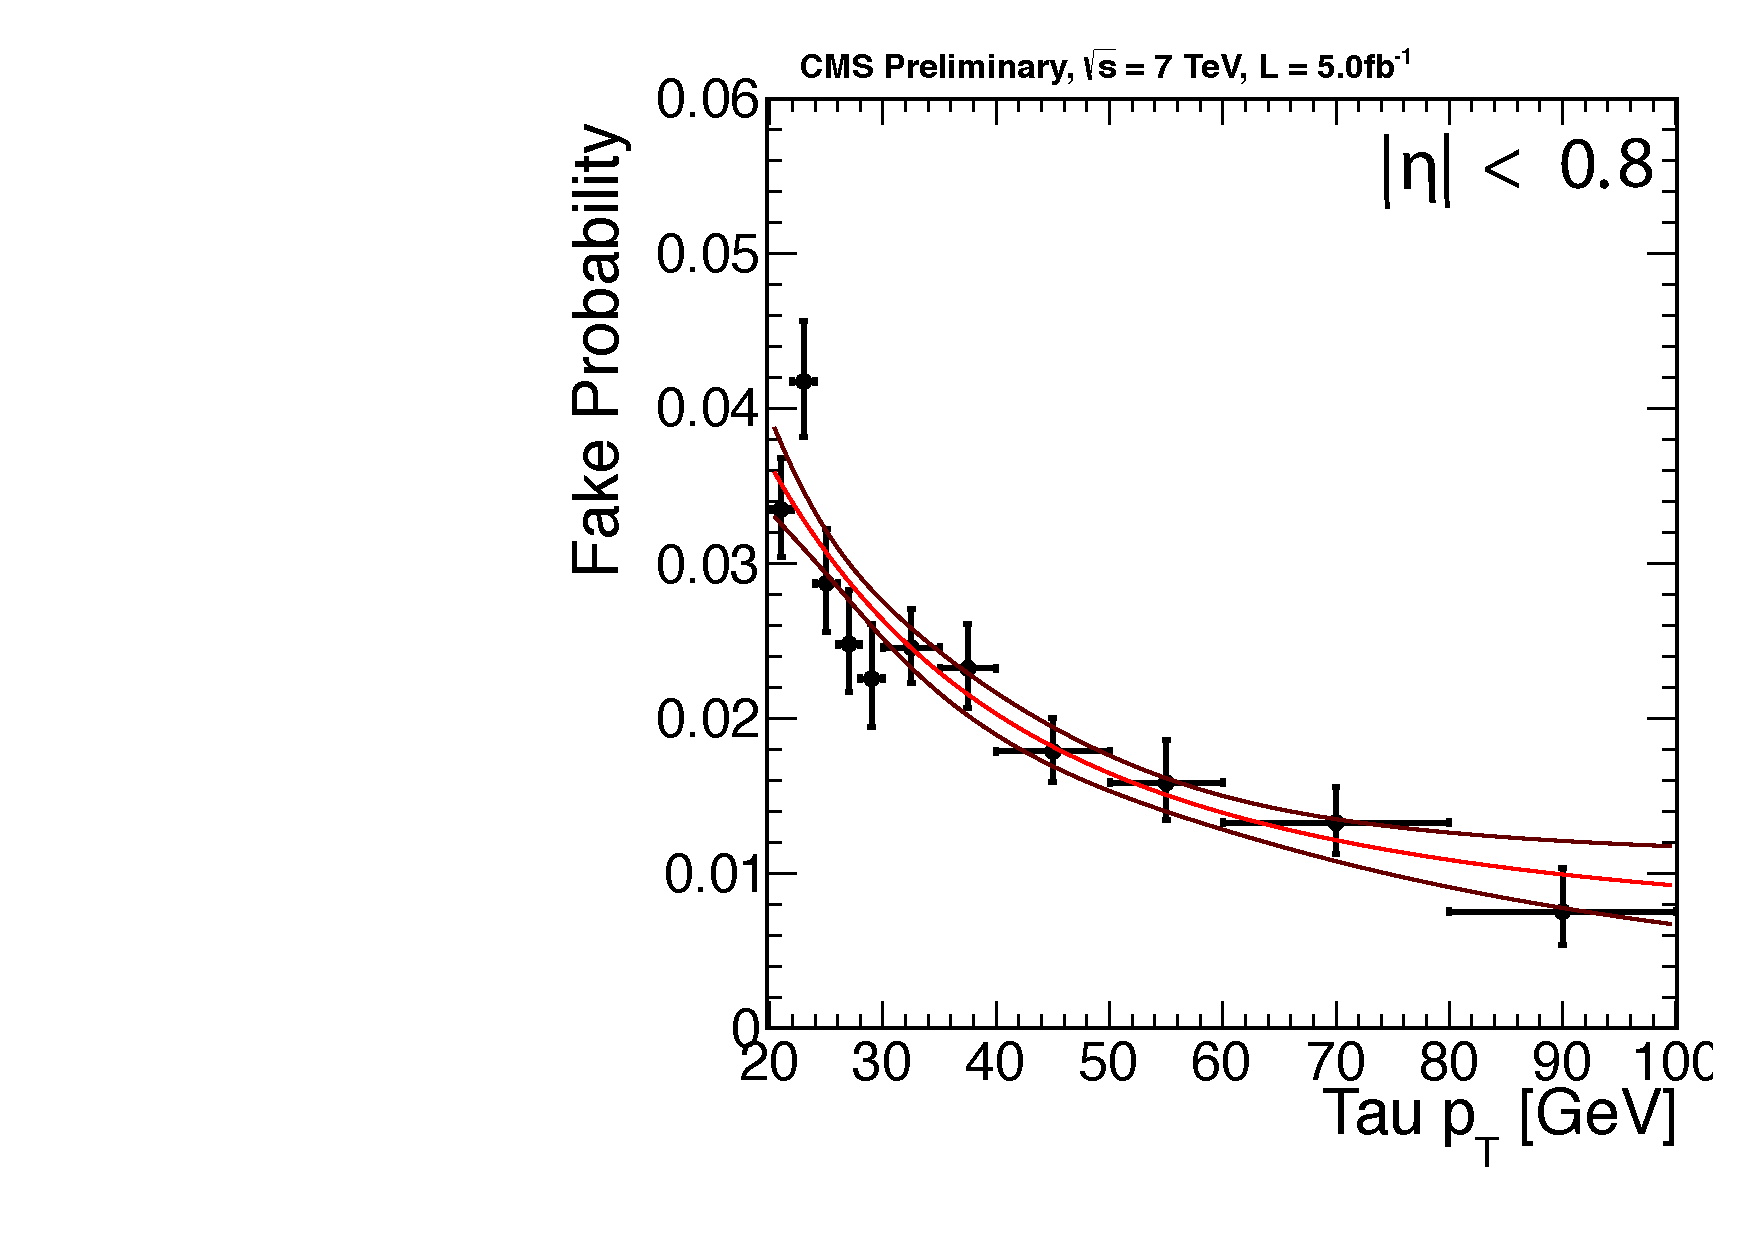
\includegraphics[width=0.33\textwidth]{4_Analisys/pics/7TeV/fakerate_fits/tau_fr_barrel.pdf}
  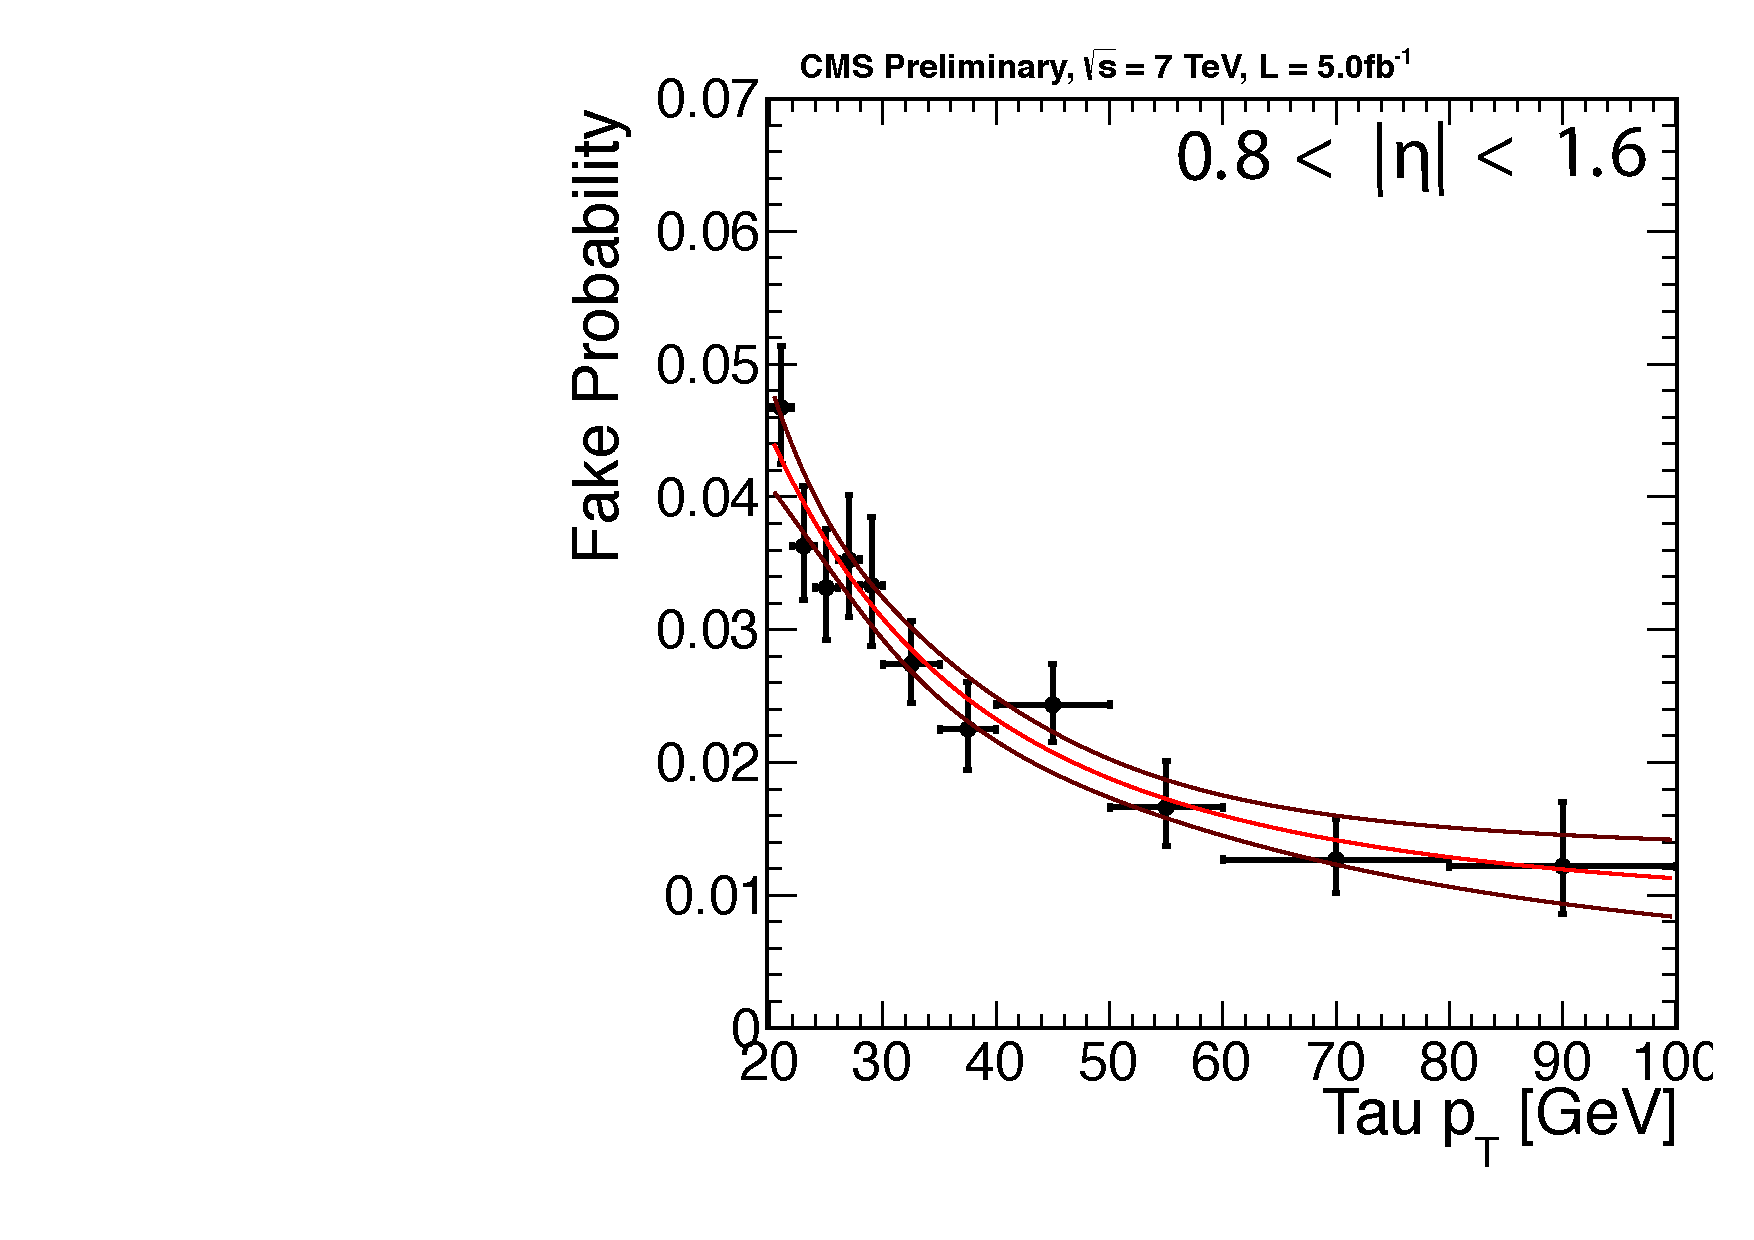
\includegraphics[width=0.33\textwidth]{4_Analisys/pics/7TeV/fakerate_fits/tau_fr_transition.pdf}
  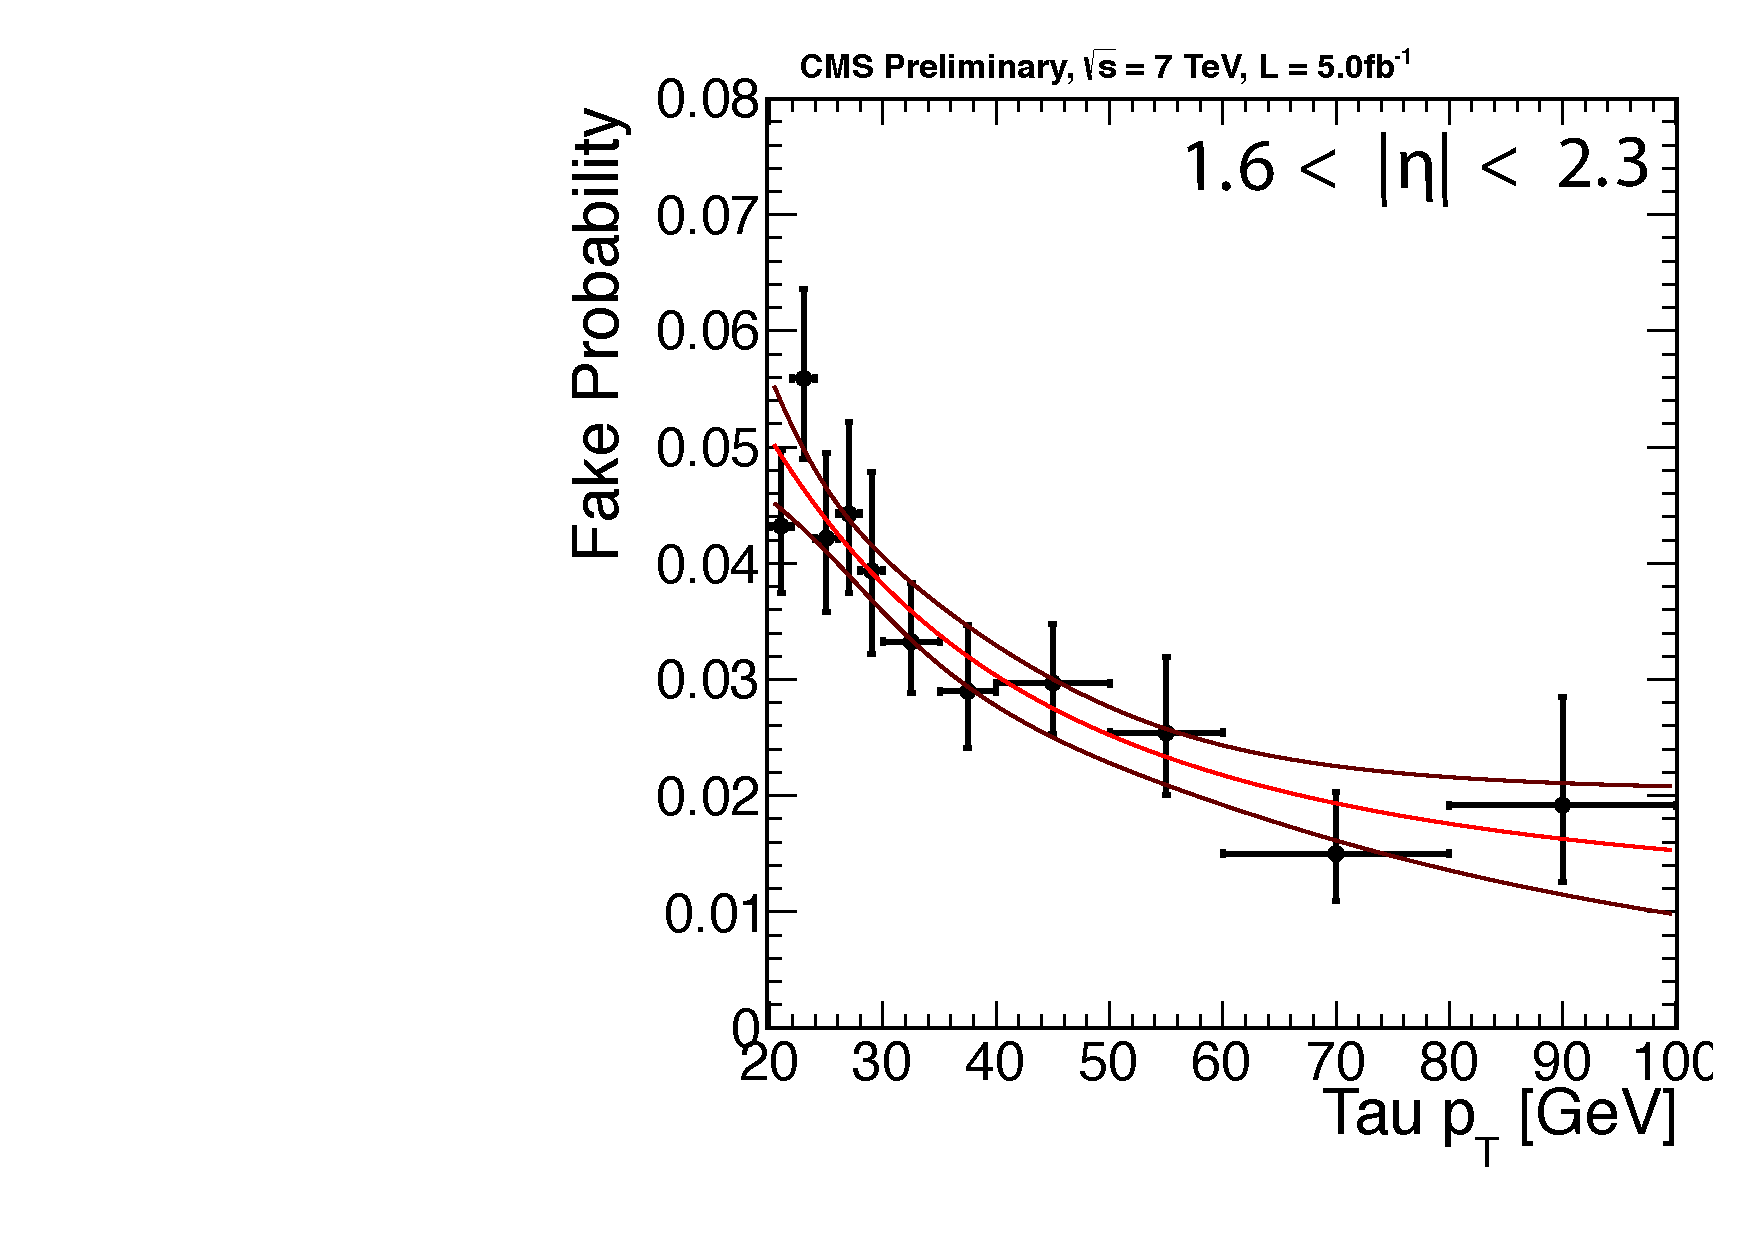
\includegraphics[width=0.33\textwidth]{4_Analisys/pics/7TeV/fakerate_fits/tau_fr_endcap.pdf}\\
  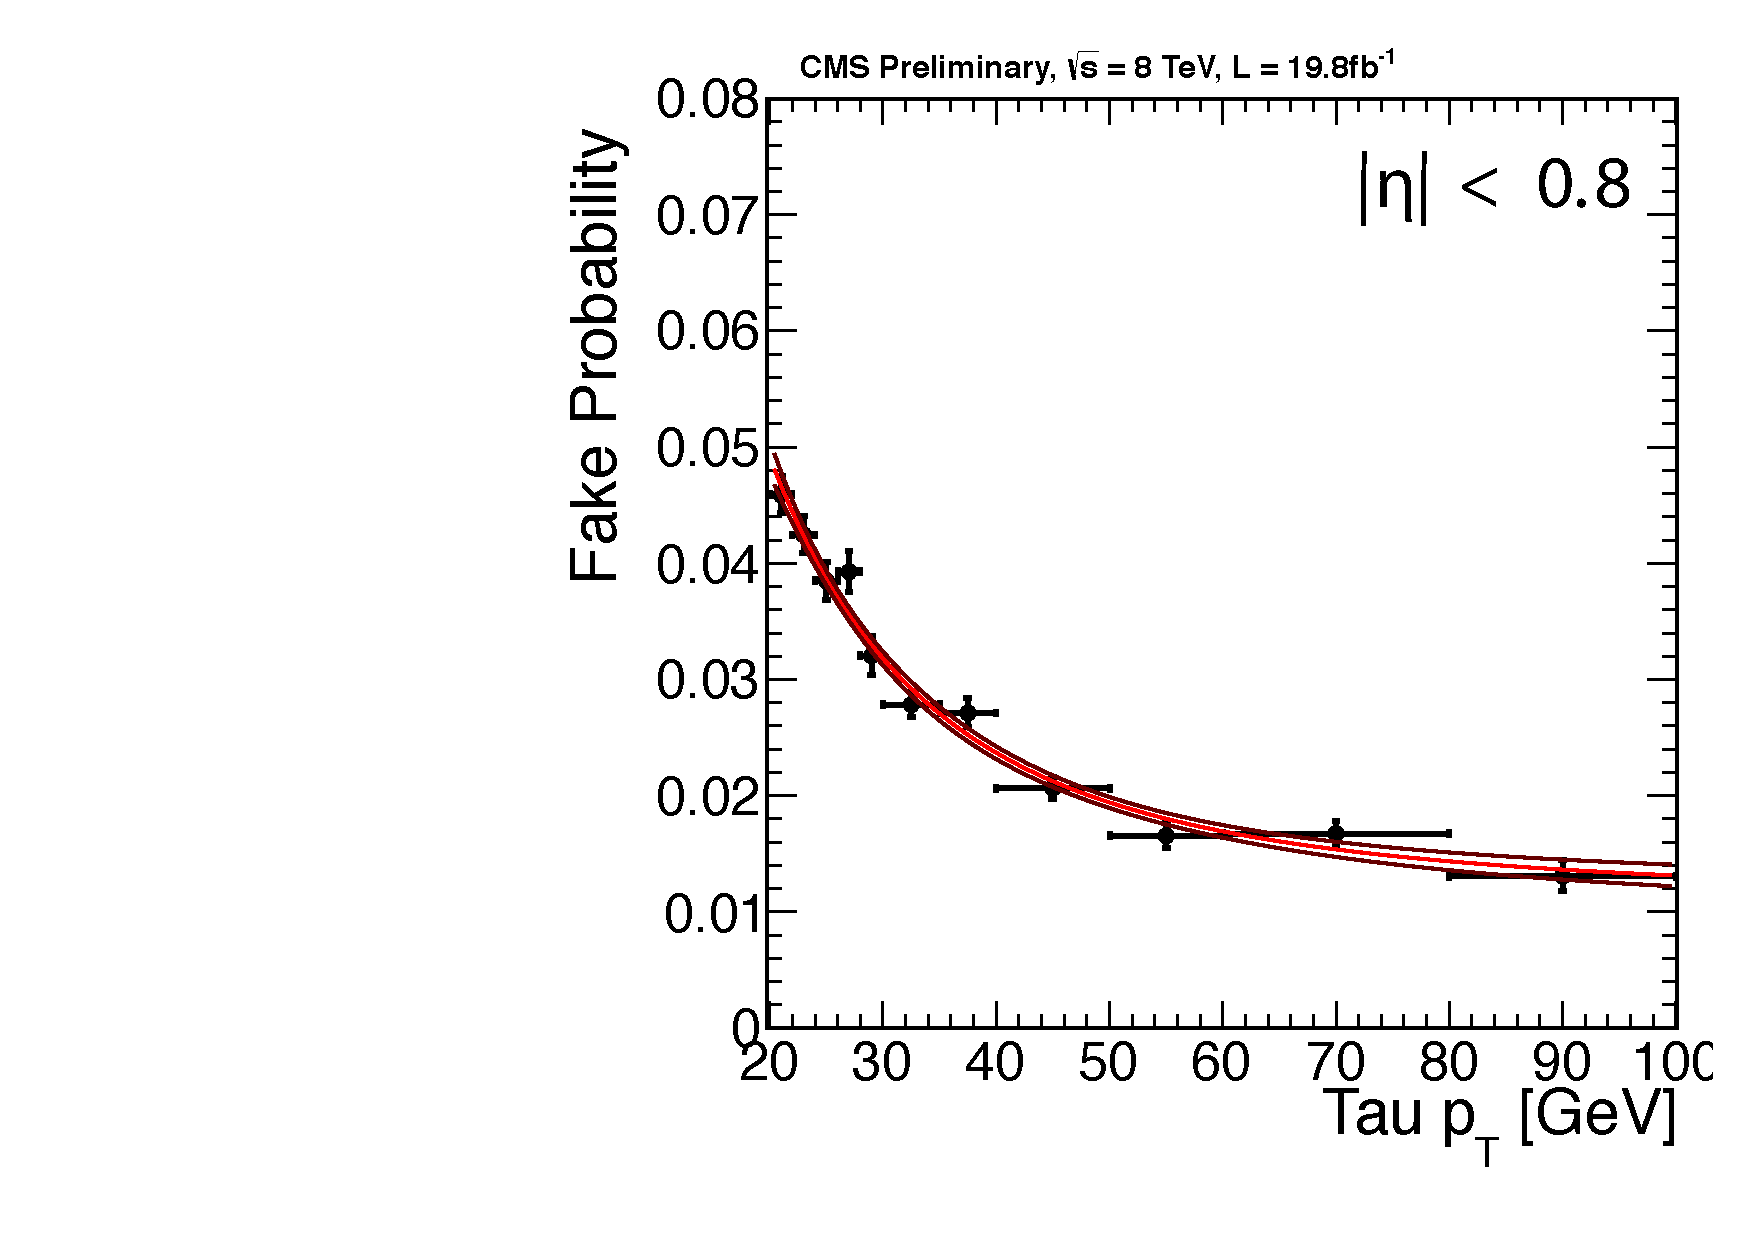
\includegraphics[width=0.33\textwidth]{4_Analisys/pics/8TeV/fakerate_fits/tau_fr_barrel.pdf}
  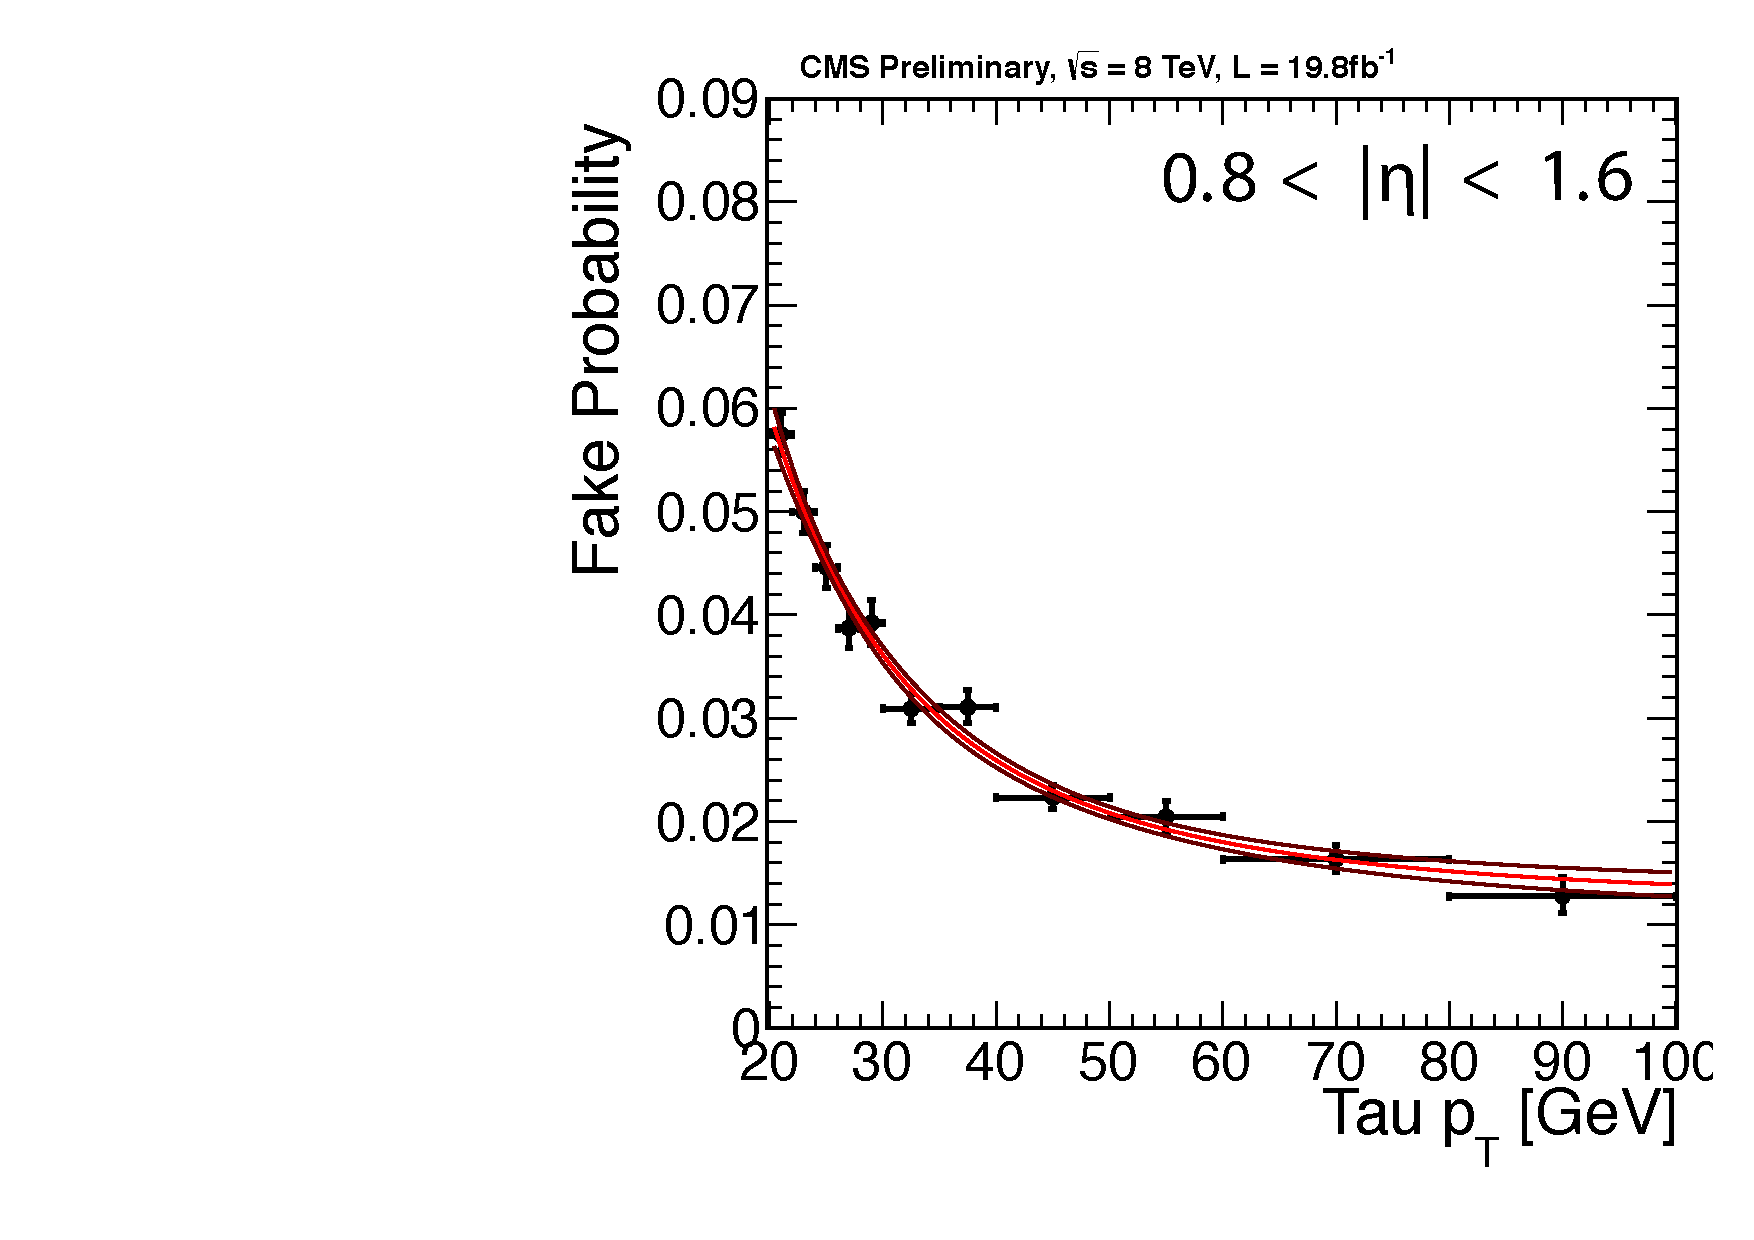
\includegraphics[width=0.33\textwidth]{4_Analisys/pics/8TeV/fakerate_fits/tau_fr_transition.pdf}
  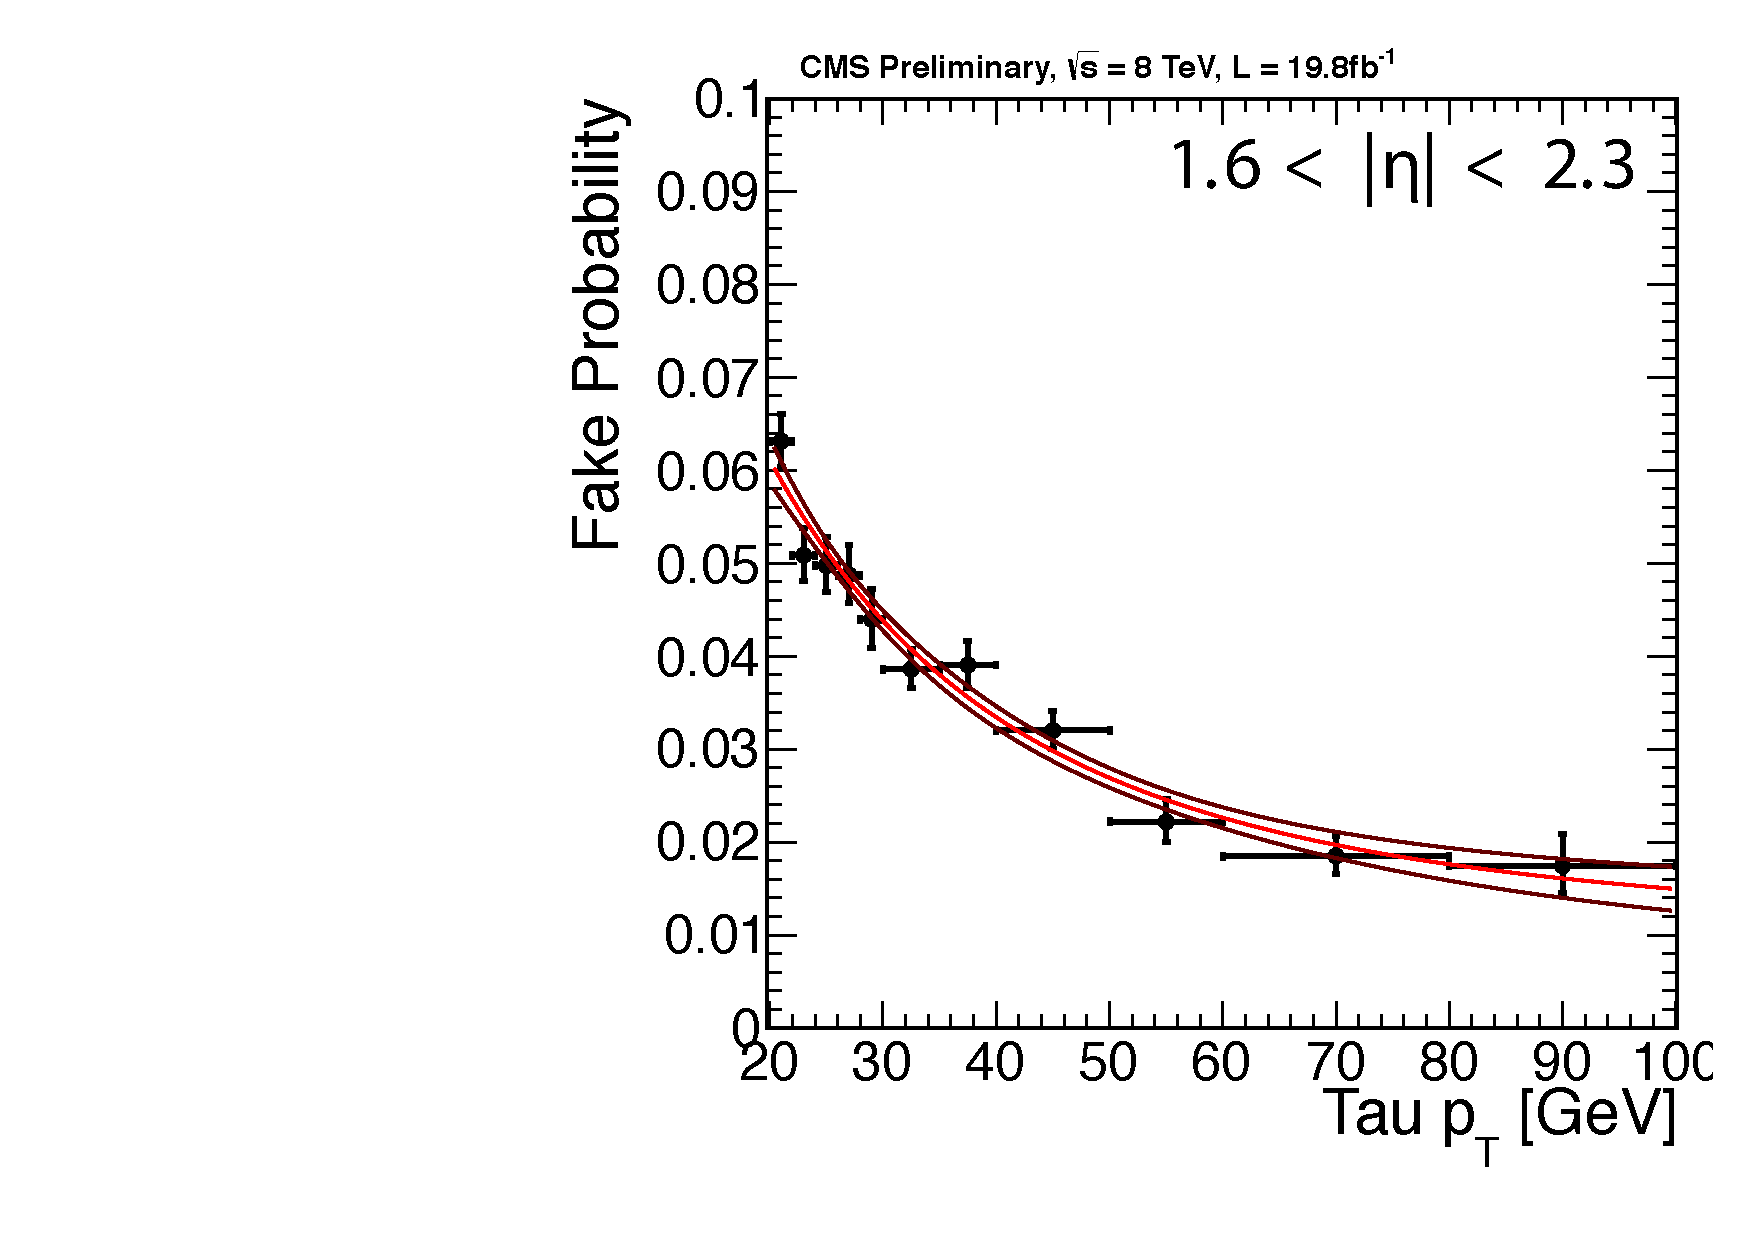
\includegraphics[width=0.33\textwidth]{4_Analisys/pics/8TeV/fakerate_fits/tau_fr_endcap.pdf}
  \caption{Jet $\to \tau_h$ misidentification rates in 7 TeV (top) and 8 TeV (bottom) data, in W$\to \mu$+jet events, versus tau \pT in barrel (left), transition (center) and endcap (right) regions.}
  \label{fig:LLT_tau_FR}
\end{figure}


\subsubsection{Background shape extraction}

The tau fake-rate is used to determine a second and completely independent estimate of the reducible background in the signal region.
In this method the tau is considered the possibly mis-identified object and events passing all the analysis selection criteria plus the loose tau
selection but \emph{not} the tight one are weighted according to the measured tau fake-rate to estimate the reducible background.

This method only takes into account those processes in which jets are misidentified as taus, but cannot account for the Drell-Yan, WW and $t\anti{t}$ reducible backgrounds,
in which the tau is either a genuine tau or a light lepton faking a tau. To account for this sources of background the method described in Section \ref{sec:fakemethod}
is applied to simulated events. This solution is considered more reliable than taking the MC expectation in the signal region directly.

The fake tau method was found to produce results consistent with the previous method. To account for possible residual differences,
the fake lepton method was used as nominal value for the reducible background and the second estimate as a shape systematic uncertainty on the background distribution shape.

\subsection{Electron charge mis-idenfication}
\label{sec:charge_misid}

The charge of an electron is incorrectly assigned mostly due to a radiative process. An electron can radiate a photon, carrying most of its momentum, which may convert into a $e^+e^-$ pair with highly unbalanced momenta, leaving the electron with opposite charge to the initial one with most of the energy. If these two processes
happen in proximity of the interaction point the reconstruction algorithm cannot identify this electron as originating from a conversion.
The description of this process in the simulation is handled by \textsc{GEANT}~\cite{geant}. The probability for an electron to be reconstructed with opposite charge is measured
with a $\Z \rightarrow ee$ MC sample as a function of the electron $\eta$ and \pT. The results are shown in Fig.~\ref{fig:charge_flip_prob_map}.

Another effect associated to this charge misassignment is a partial energy loss through radiation is not associated to the electron candidate.
This effect causes a shift of the dielectron invariant mass spectrum.
The precision with which this phenomenon is modeled in the simulation is not totally satisfactory. To quantify this effect the spectra of opposite sign (OS) and same sign (SS) electron pairs were fitted with a Cruijfian function allowing only a global scaling factor to float. The results of these fits is shown in Fig.~\ref{fig:ee_invMass_fit}. The process is repeated for both data and simulated events. The value extracted from the former is taken as central value, while the one taken from the latter is used as systematic uncertainty.

\subsection{Control regions}

The background induced by charge misassignment is validated in a dedicated $\Z \To e^\pm e^\pm$ control region.
This region has the same selection as the $ee\tau_h$ signal region with the exception that events containing a tau are removed.
The di-electron invariant mass spectrum in this region is shown in Fig.~\ref{fig:control_Zee}. The red histogram represents opposite-sign dielectron events weighted by the charge misassignment probability and with the invariant mass scaled by an offset extracted from MC simulation.

\begin{figure}
  \begin{center}
  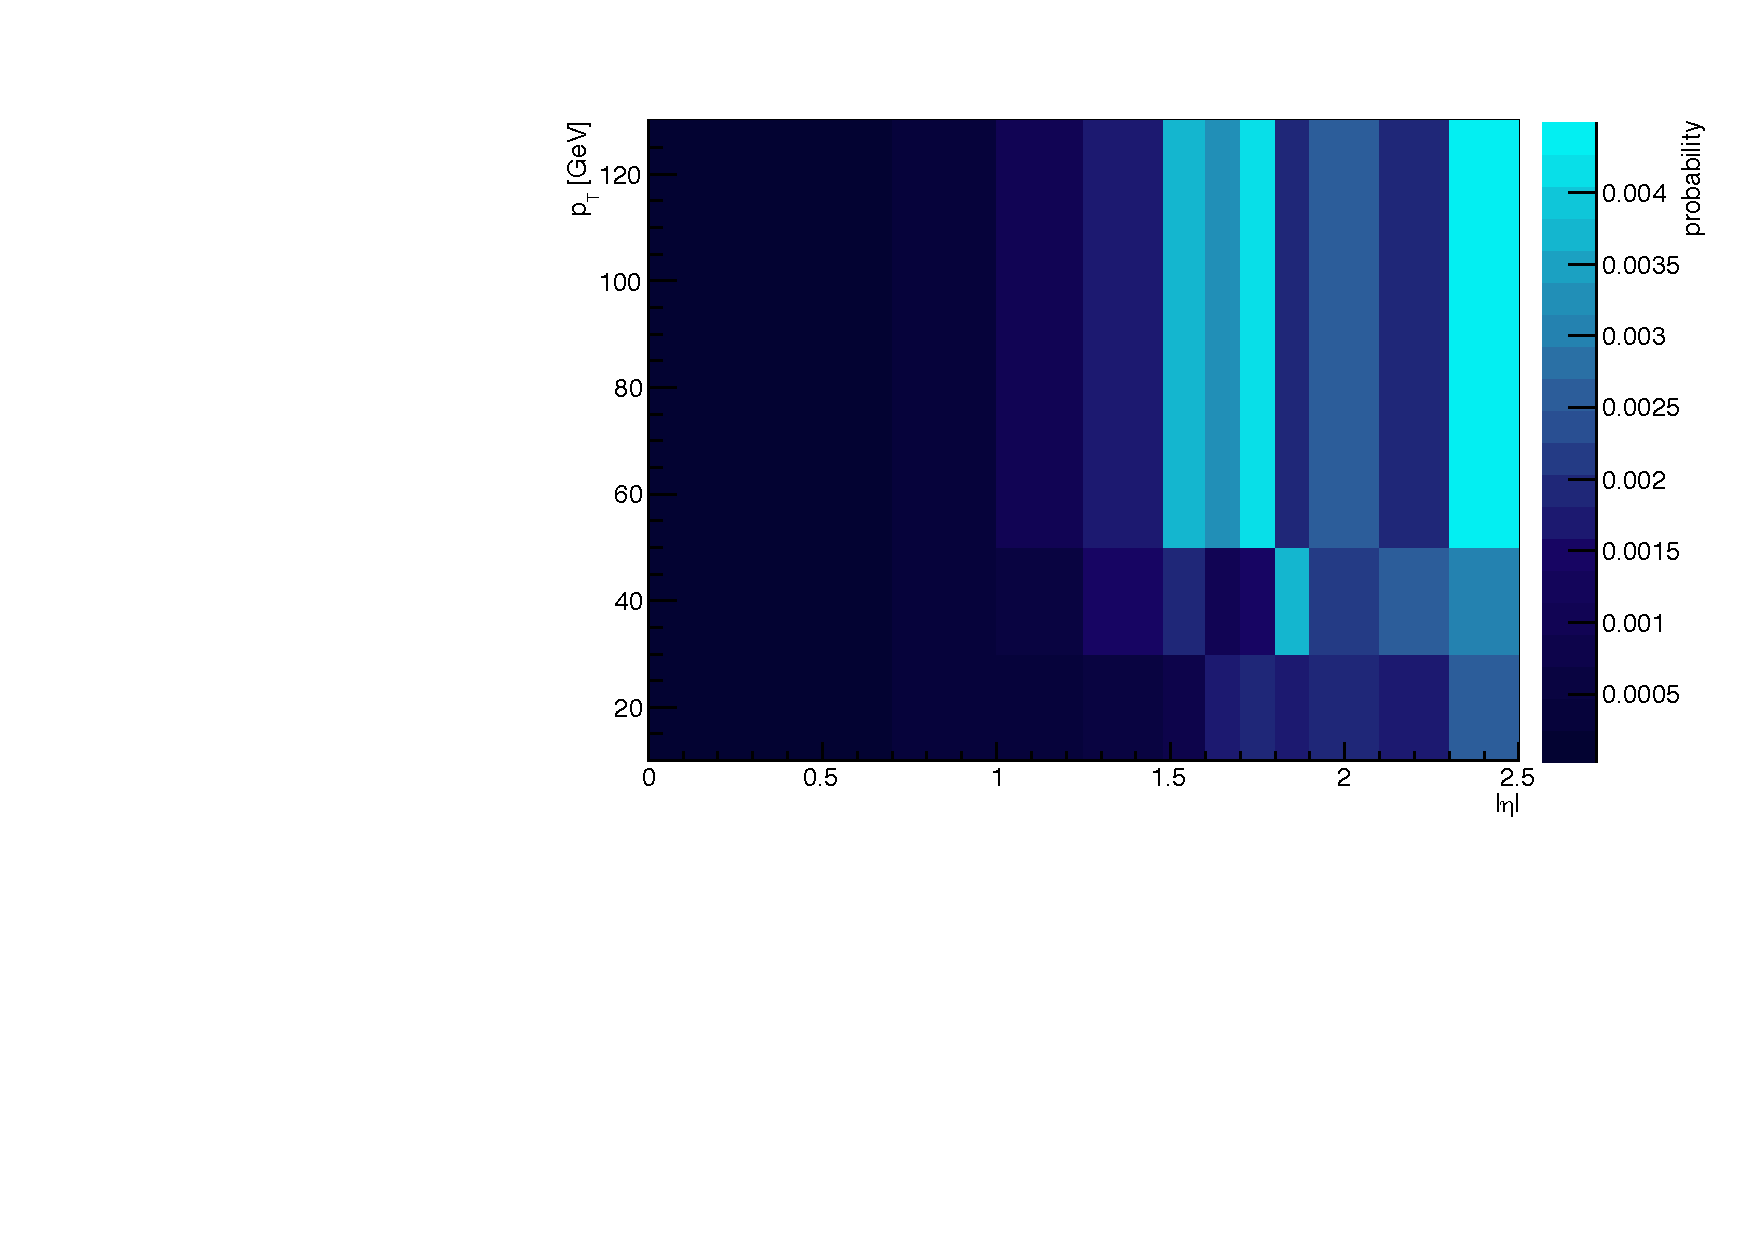
\includegraphics[width=0.8\textwidth]{4_Analisys/pics/8TeV/fakerate_fits/charge_flip_prob_map_eid12Medium_h2taucuts.pdf}
  \caption{
  Electron charge misassignment probability (color scale) as a function of $|\eta|$ and \pT.}
  \label{fig:charge_flip_prob_map}
  \end{center}
\end{figure}


\begin{figure}
  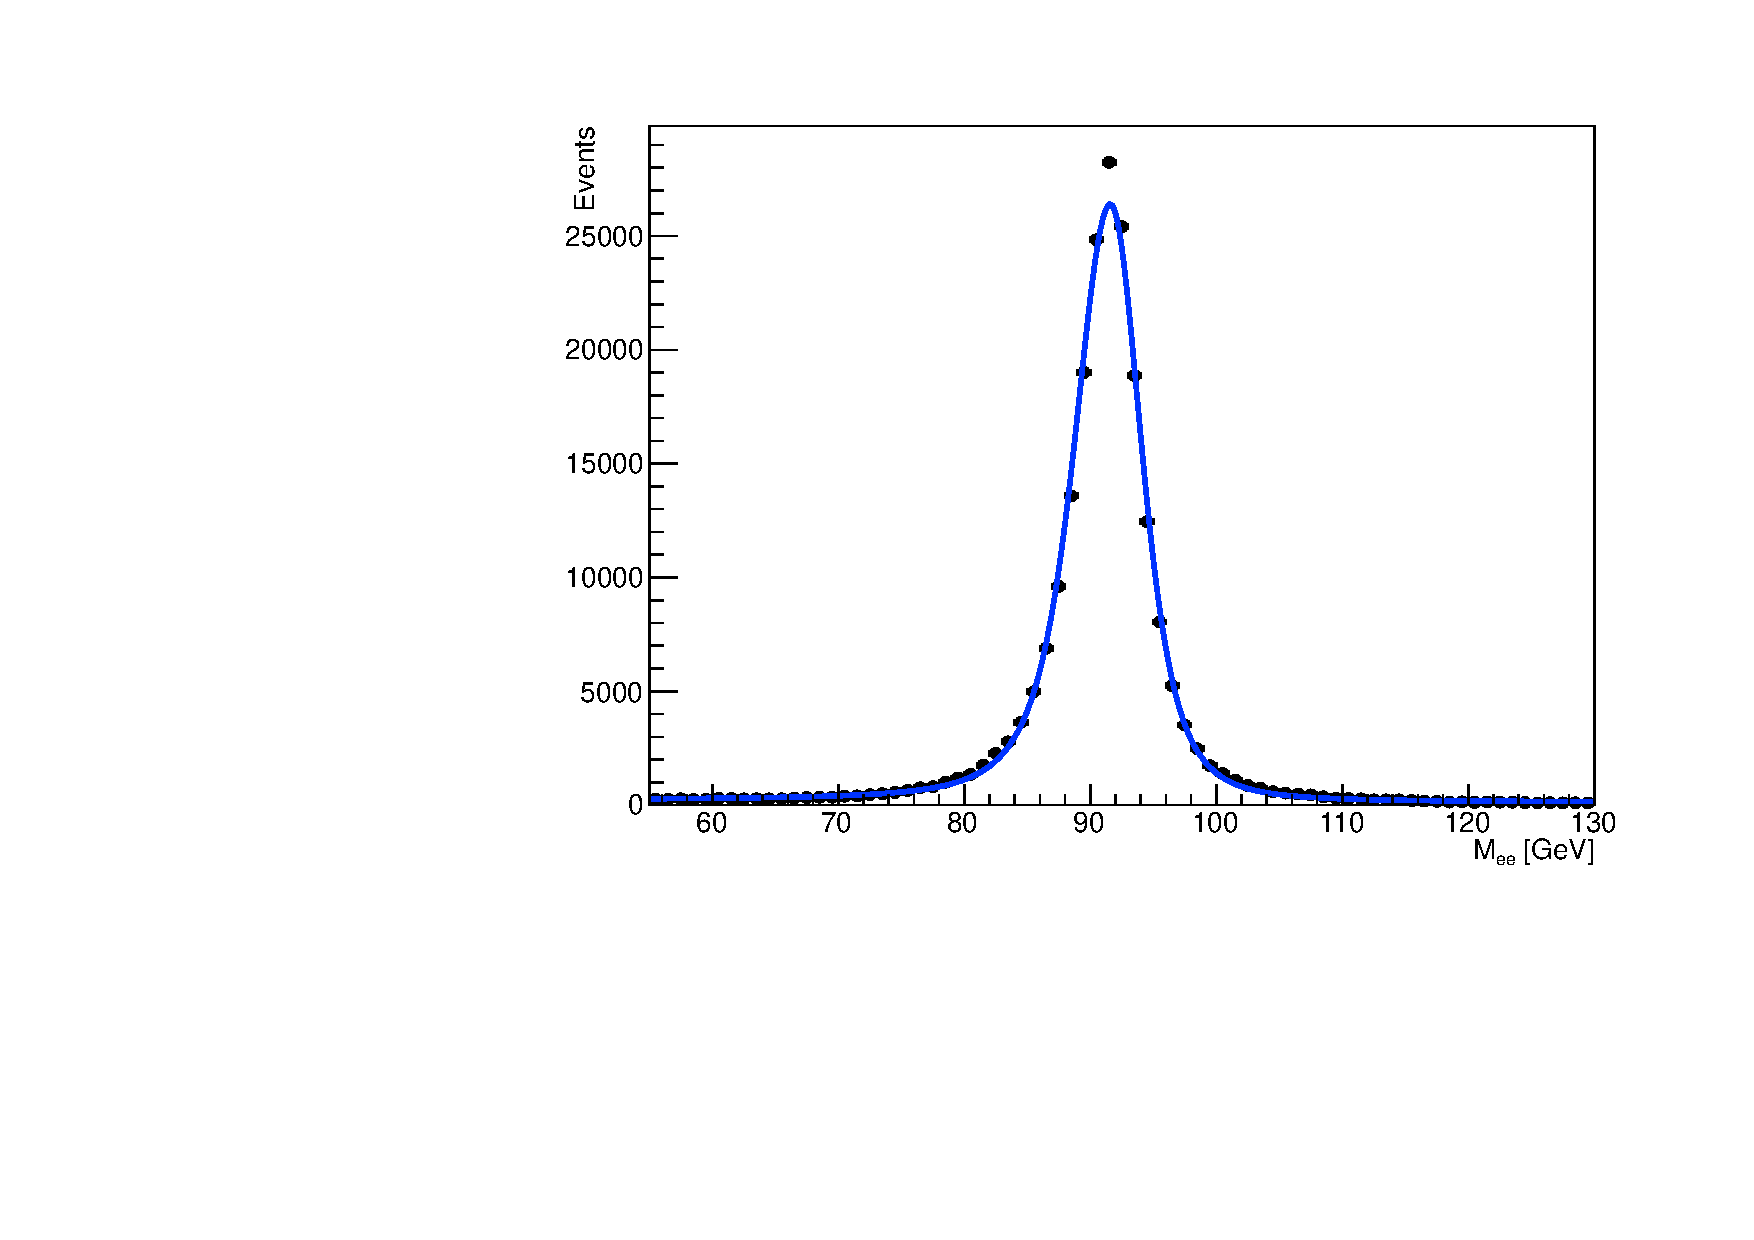
\includegraphics[width=0.5\textwidth]{4_Analisys/pics/8TeV/fakerate_fits/charge_flip_prob_map_eid12Medium_h2taucutsos_trkMass.pdf}
  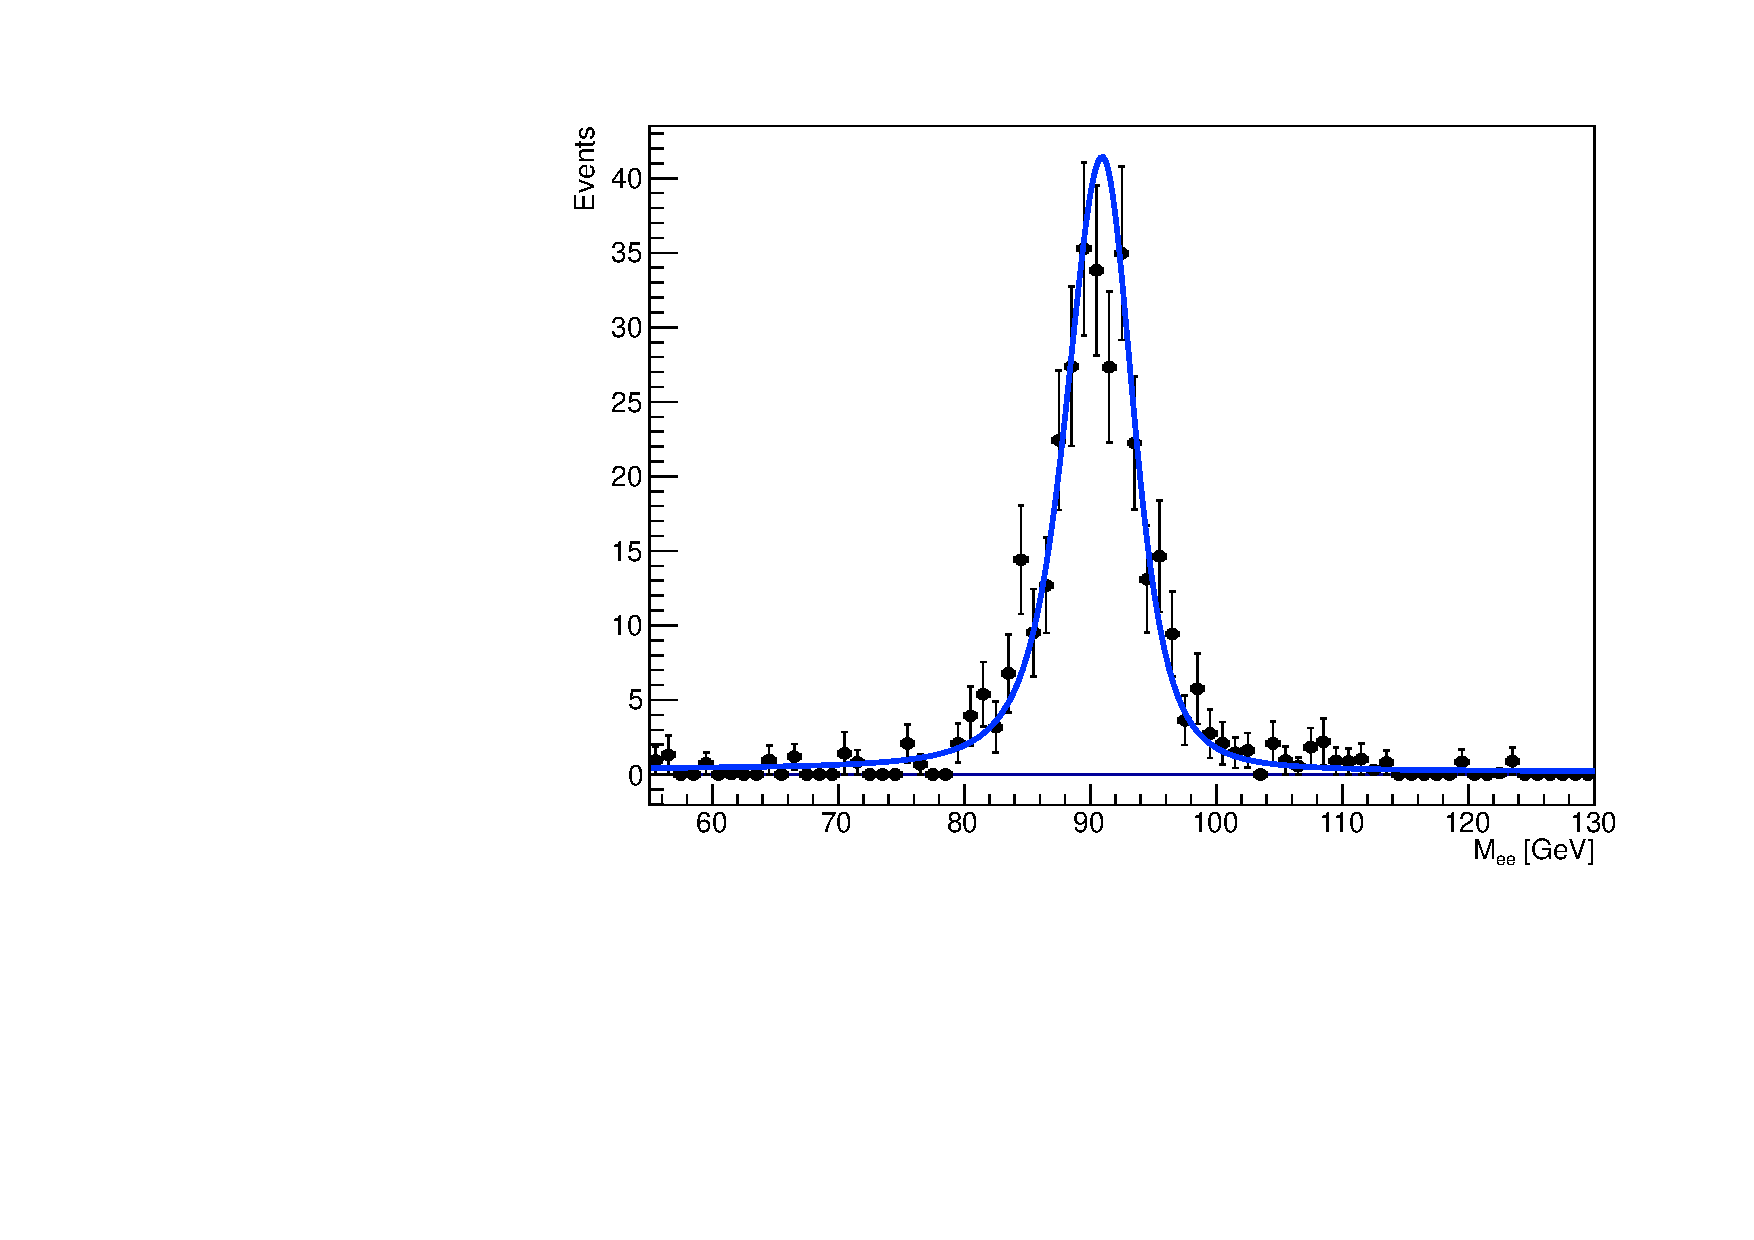
\includegraphics[width=0.5\textwidth]{4_Analisys/pics/8TeV//fakerate_fits/charge_flip_prob_map_eid12Medium_h2taucutsss_trkMass.pdf} \\
  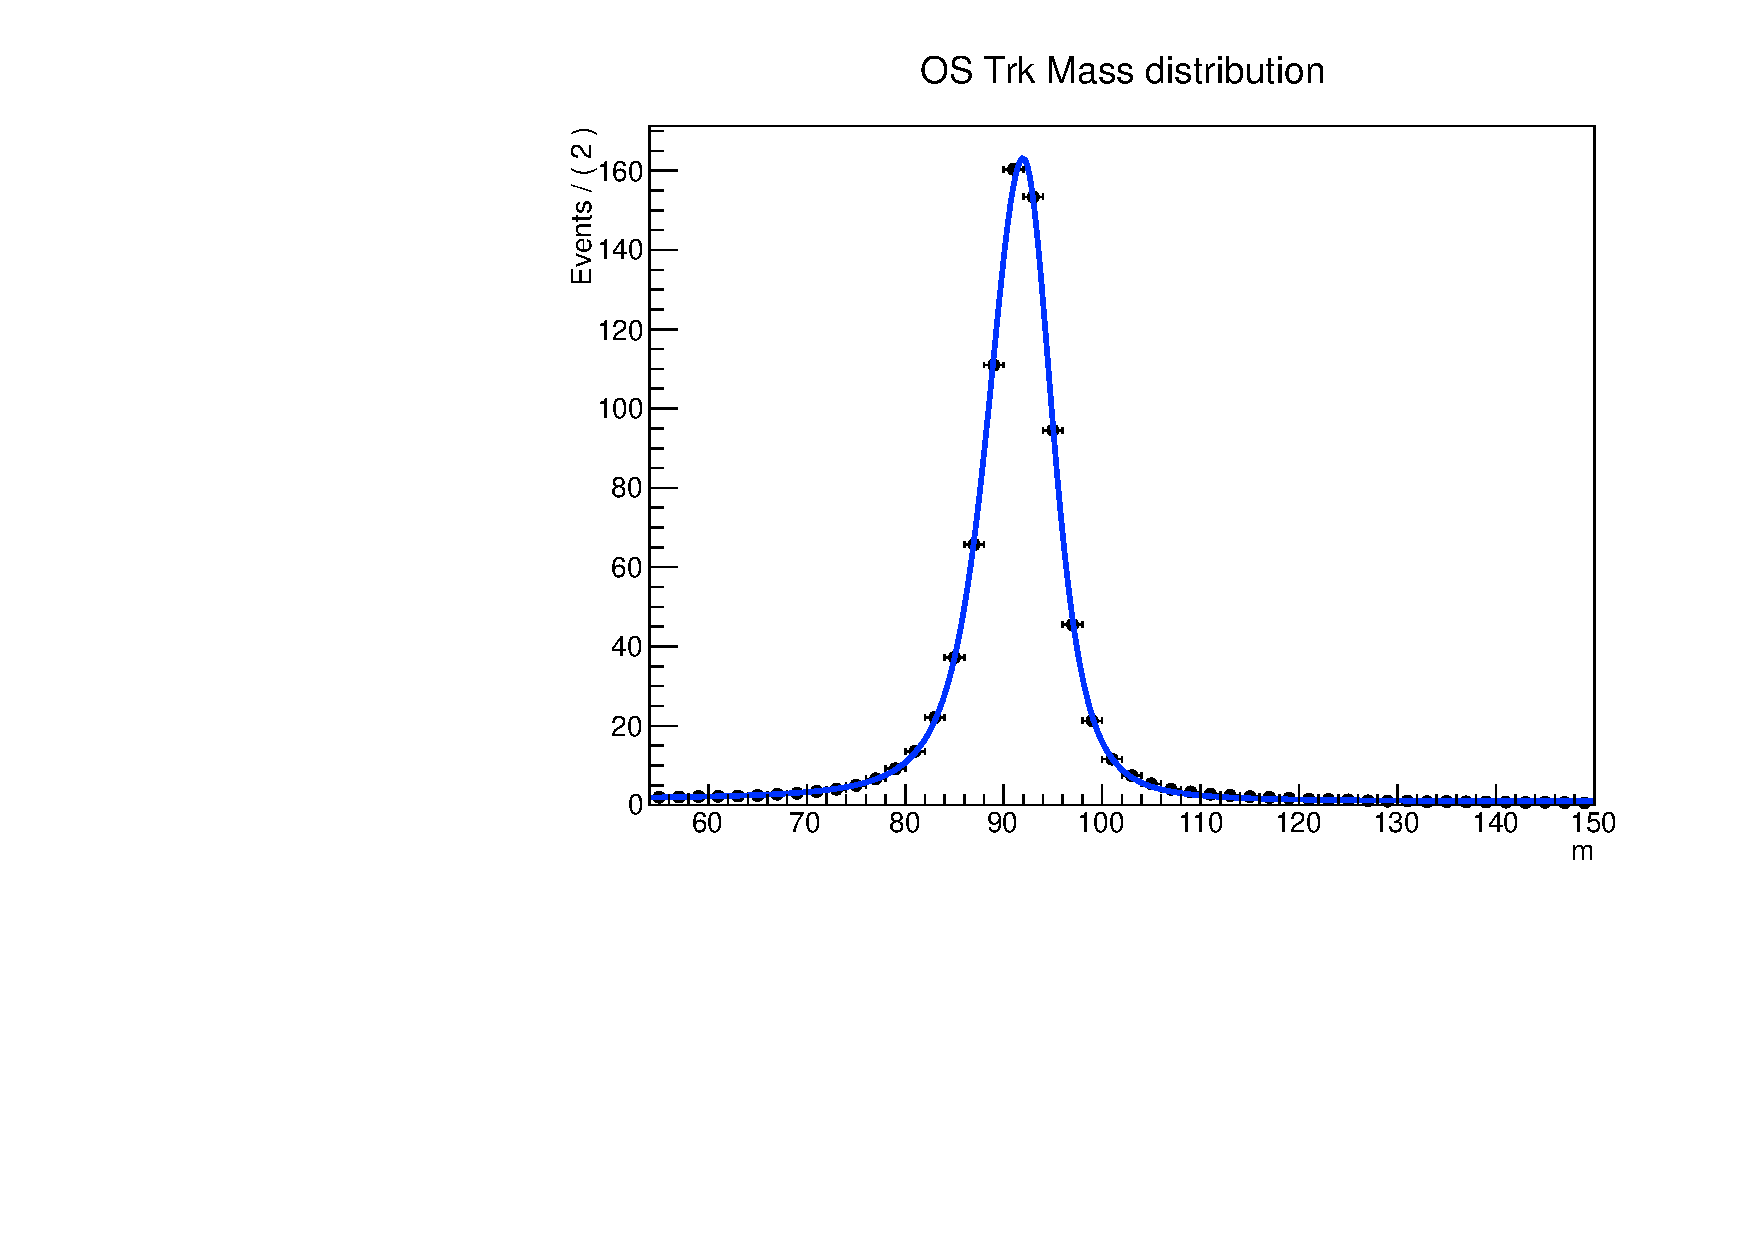
\includegraphics[width=0.5\textwidth]{4_Analisys/pics/8TeV/fakerate_fits/charge_flip_prob_map_dataos_trkMass.pdf}
  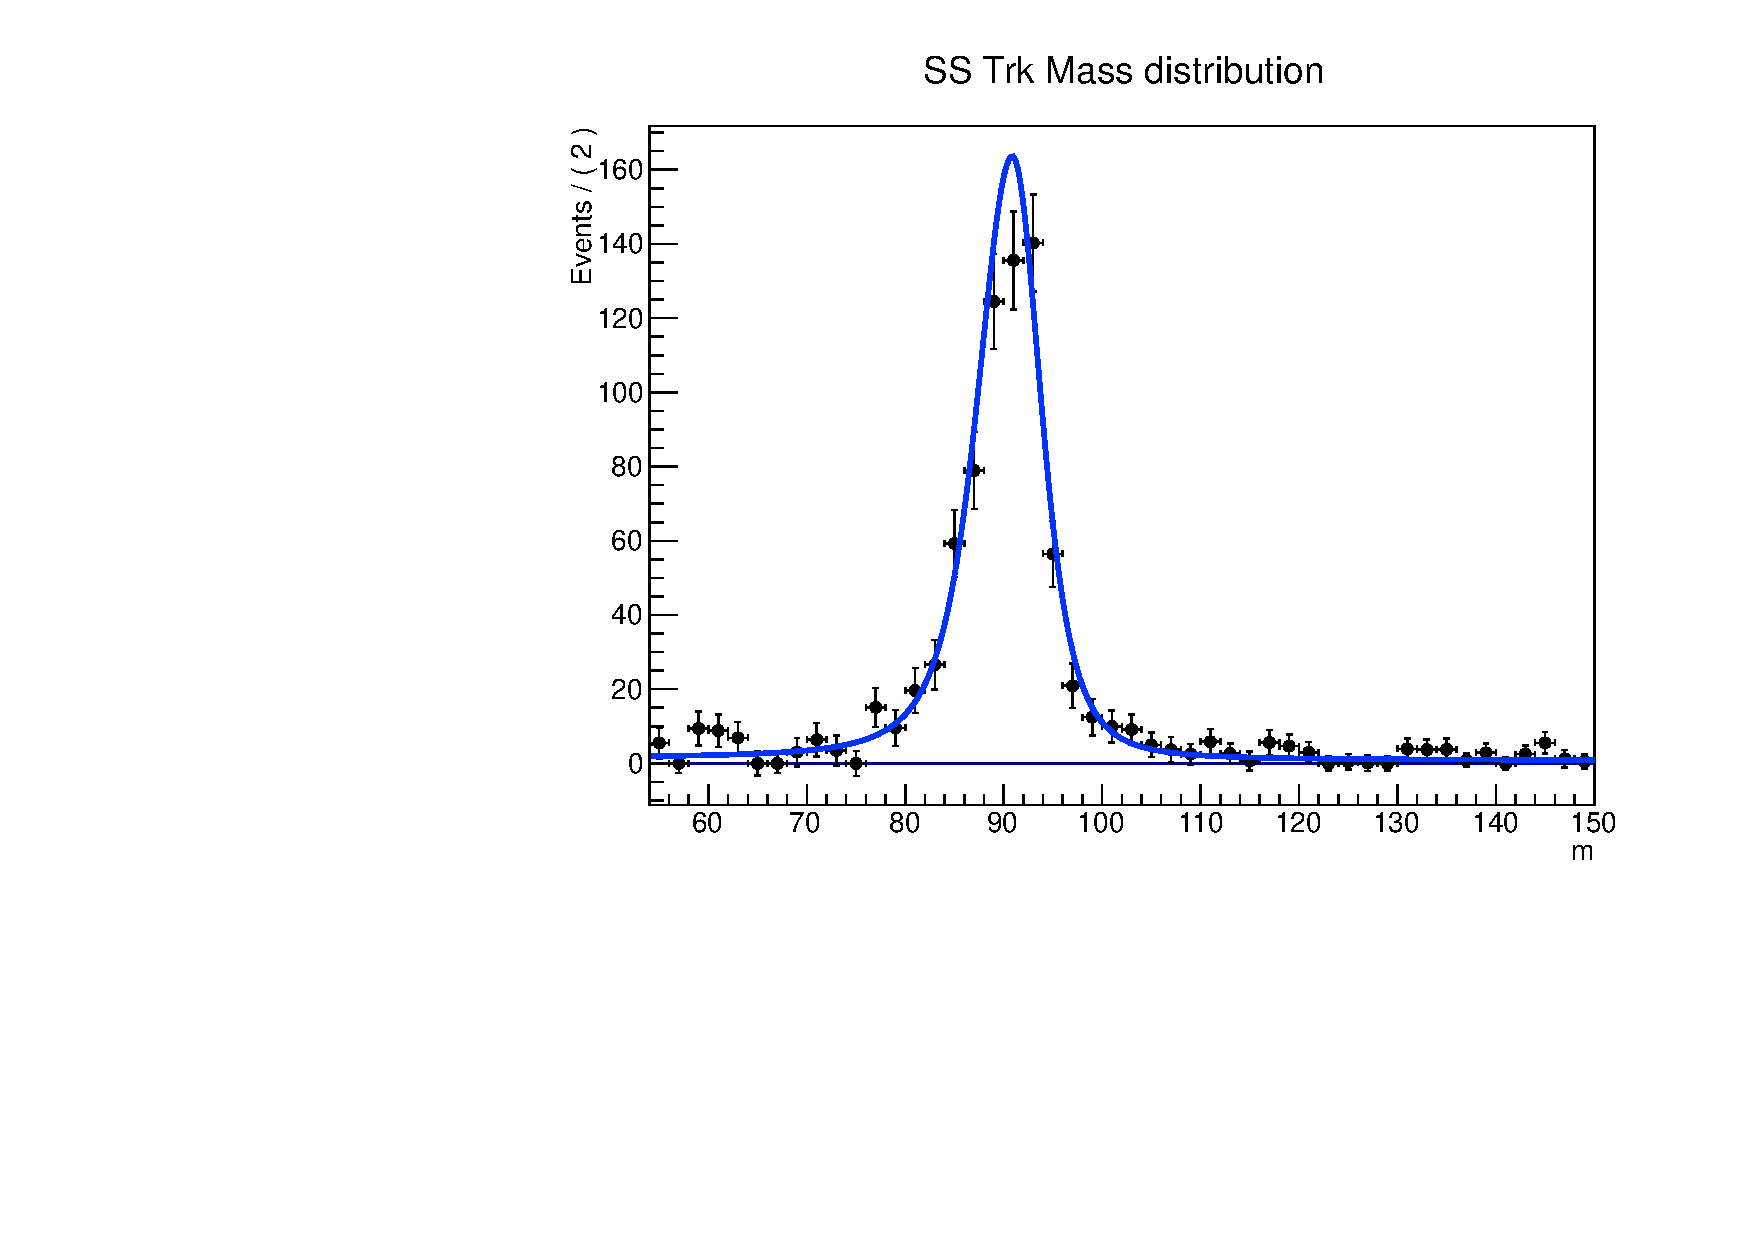
\includegraphics[width=0.5\textwidth]{4_Analisys/pics/8TeV//fakerate_fits/charge_flip_prob_map_datass_trkMass.pdf} \\  
  \caption{
  Comparison of the fit to dielectron invariant mass distributions opposite sign (left) and same sign (right) dielectron candidates from Drell--Yan simulation (top) and $\Z\To ee$ data (bottom). The measured invariant mass scale factor is 0.7\% for simulated events and 1.2\% for data}
  \label{fig:ee_invMass_fit}
\end{figure}

\begin{figure}
  \begin{center}
  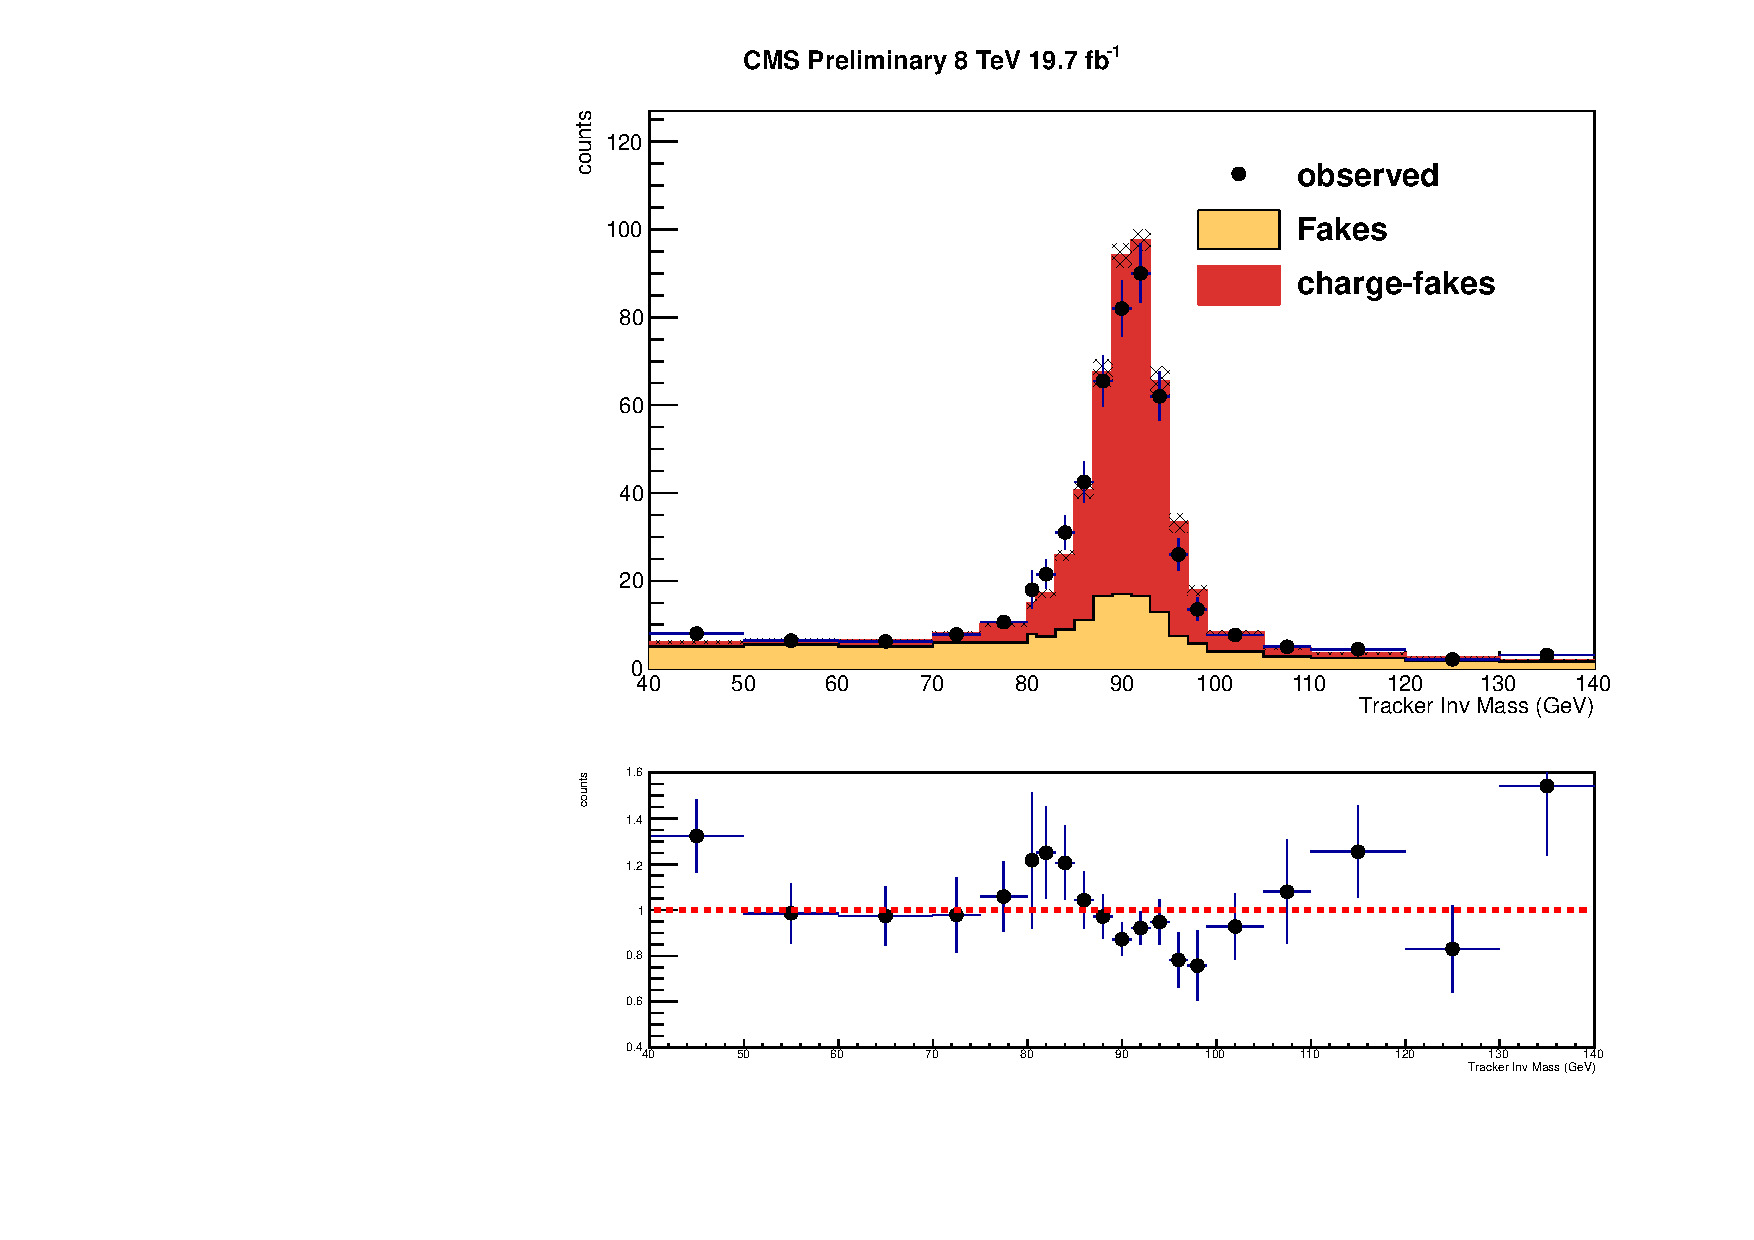
\includegraphics[width=0.8\textwidth]{4_Analisys/pics/8TeV/plots/zee/EE_Charge_Flip_xcheck_trk_invMass.pdf}
  \caption{Invariant mass distribution of same sign di-electron events: the red histogram is obtained using the information extracted from simulation
(charge misassignment probability and invariant mass scale correction) and applying them to opposite--sign data, the yellow histogram is obtained applying the fake lepton method to estimate the reducible background.}
  \label{fig:control_Zee}
  \end{center}
\end{figure}

\section{Systematics uncertainties and category optimization}
\label{sec:systematics}

The optimization of the analysis sensitivity and the description of the systematic uncertainties are two subjects tightly bound. The figure of merit to maximize in the optimization process is the expected signal significance while considering the full set of uncertainties correlated for both signal and backgrounds. An optimization purely based on the ``statistical'' significance, defined as $S = N_{sig} / \sqrt{N_{sig} + N_{bkg}}$ may indeed yield as optimal a configuration where the systematic uncertainties are very large.

In this section I will briefly introduce the definitions and values necessary to have a complete picture of the category optimization process. The systematic uncertainties are described after the optimization process.
%Once this process will have been fully detailed a more complete description of the systematic uncertainties and their values will be presented. 
A detailed description of how systematic uncertainties are treated to obtain the final result is left for the sections describing the statistical interpretation of the data.

\subsection{Category optimization}

Given the strong dependence of the mis--identification rate on the \pT of the object considered, in particular the hadronic tau, it is quite straightforward to try to improve the signal purity by increasing the threshold on the objects \pT. A better but correlated solution is to use as discriminating observable the scalar sum of the \pT of the three final state leptons, called $L_T$.  

Two types of systematic uncertainties on <in/> the background templates are considered in this analysis: normalization uncertainties, which affect only the total yield of a background, and shape uncertainties, which also affect relative yields between bins.

Normalization uncertainties are assigned to account for uncertainties in the luminosity measurement, the correction factors for the trigger emulation, in the identification and isolation efficiencies and in the theoretical cross-section measurement for all the simulated processes. Normalization uncertainties are also assigned to account for the limited size of the MC samples and the very limited size of the loose-but-not-tight samples that are used to estimate the reducible backgrounds. The last two sources of background are strongly dependent on the category selection and have to be dynamically assigned to each tested configuration.

The difference between the reducible background shape computed with the fake lepton method and the one evaluated with the fake tau is accounted for with a shape uncertainty allowed to vary both the shape and the normalization of the background. The same procedure is applied to the reducible background shapes computed with the optimal number of neighbors and the two inferred boundaries. Single bin fluctuations in the reducible background shape due to the limited statistics in the anti--isolated regions are separately accounted by several shape uncertainties (also called \emph{bin--by--bin uncertanties}). These shape bin--by--bin uncertainties are not allowed to change the total yield of the background process, as this effect is collectively handled by the appropriate normalization uncertainty. It is evident that also these shape uncertainties are dependent on the category selection.

During the optimization two options were tested: either apply a cut rejecting all the events below a certain \LT threshold, or divide the events in two categories (called \LT--high and \LT--low) that get fitted simultaneously, increasing the total sensitivity of the analysis. For each \LT \ threshold tested the expected frequentist significance of both options has been computed for a SM Higgs boson of 125 GeV. The \LT\ scan was performed varying the threshold between 60 and 170 GeV in 10 GeV steps. 

The categorization performs \emph{at least} as well as the equivalent cut option, since the \LT--high category has the same statistical power of the only category in the cut case. The categorization choice, however, requires a significant amount of data in both the event categories to be stable. Due to <For/> this reason the categorization option has not been investigated in the 7 TeV data. In the 8 TeV $ee\tau_h$ channel the difference between the two options was found to be negligible and therefore the more simple cut was chosen. Figure \ref{fig:LT_scan} show the results of the threshold scans for three channels in the two run periods, while Table \ref{tab:LT_options} shows the \LT\ threshold values that maximize the significance for each channel, the reported selection is used to extract the final result.

\begin{figure}
  \includegraphics[width=0.5\textwidth]{4_Analisys/pics/7TeV/limits/mmt.pdf}
  \includegraphics[width=0.5\textwidth]{4_Analisys/pics/8TeV/limits/mmt.pdf} \\
  \includegraphics[width=0.5\textwidth]{4_Analisys/pics/7TeV/limits/emt.pdf}
  \includegraphics[width=0.5\textwidth]{4_Analisys/pics/8TeV/limits/emt.pdf} \\
  \includegraphics[width=0.5\textwidth]{4_Analisys/pics/7TeV/limits/eet.pdf}
  \includegraphics[width=0.5\textwidth]{4_Analisys/pics/8TeV/limits/eet.pdf} \\
  \caption{Expected significance versus \LT threshold for the $\mu\mu\tau_h$ (top), $e\mu\tau_h$ (center), and $ee\tau_h$ (bottom) in 7 TeV (left) and 8 TeV (right) running periods for two optimizations. The variation of the LT threshold is represented by the black dots, the separation of LT event categories by the red points.}
  \label{fig:LT_scan}
\end{figure}

\begin{table}
\begin{center}
\caption{Systematic uncertainties affecting the $2\ell\tau_h$ categories.  Where the value used in 2012 differs from 2011, it is indicated in parenthesis.}
\label{tab:LT_options}
\begin{tabular}{c c c c}
\hline
Run period & Channel & Best approach & Threshold (GeV) \\
\hline
\multirow{3}{*}{ 7 TeV } & $\mu\mu\tau_h$ & \LT\ Cut & 80 \\	
& $e\mu\tau_h$ & \LT\ Cut & 90 \\
& $ee\tau_h$    & \LT\ Cut & 90 \\
\hline
\multirow{3}{*}{ 8 TeV } & $\mu\mu\tau_h$ & \LT\ Category & 100 \\	
& $e\mu\tau_h$ & \LT\ Category & 110 \\
& $ee\tau_h$    & \LT\ Cut & 70 \\
\hline
\end{tabular}
\end{center}
\end{table}


\subsection{Systematic uncertainties}

As previously described, the sources of systematic uncertainties accounted for in this work can be divided into two groups: the ones affecting only the total normalization of a process, yielding a normalization uncertainty, and the ones also affecting the distribution of the events, yielding a shape uncertainty.

A 2.2\% (2.6\%) uncertainty~\cite{lumi-uncertainty} on <in/> the total integrated luminosity is applied to the 7 TeV (8 TeV) simulated samples, respectively. This uncertainty is correlated throughout all the simulated processes, categories and channels belonging to the same running period.
The theoretical uncertainties accounted for the diboson cross-sections are 4\% due to parton distribution function (PDF) and 4\% due to the QCD renormalization scale. These uncertainties are correlated between all the diboson processes, regardless of channel, category or running period.

The statistical power of the different simulated samples are accounted for by a normalization uncertainty, varying between 3 and 10\%, uncorrelated between all the channels and categories.

The theoretical uncertainty on the signal cross section due to the unknown QCD scale and parton distribution function is 2.7\%~\cite{LHCHiggsCrossSectionWorkingGroup:2011ti}.

The uncertainties on the $e$ and $\mu$ identification, isolation, and trigger efficiencies correspond to the uncertainties on the data-to-simulation correction factors, which have been measured using a tag-and-probe technique. In a similar way to what has been performed on taus and described in Section \ref{sec:tauid_eff}, $\Z \To \ell \ell$ events are selected with a single lepton trigger and the desired isolation and identification working points are applied on both leptons. Additionally the invariant mass of the two leptons is required to fall in the mass window of the Z boson: $60 < m_{\ell\ell} < 120$. The trigger efficiencies are computed by applying the trigger requirement on the probe lepton, which does not fire the initial trigger, both on data and MC. The discrepancies between the two efficiencies, binned in \pT and $\eta$ of the lepton, are applied as a scale factor on the MC and the uncertainty on such correction are taken as systematic uncertainties. A similar tag--and--probe approach on $\Z \To \ell \ell$ events is taken also to correct for discrepancies in the identification and isolation efficiencies.
The uncertainty on the $\tau$ identification efficiency is 6\%~\cite{CMS-PAS-TAU-11-001}.
The effect on the simulated yields due to the uncertainty on the electron and $\tau_h$ energy scale has been evaluated.
The electron energy scale uncertainty (1\% for $|\eta| < 1.5$, 2.5\% elsewhere) does not have a measurable effect on the analysis.
Varying the $\tau_h$ energy scale (within a 3\%~\cite{H_tautau} uncertainty) is found to change the expected yields by $3\%$, but has no sizable effect on the observables shapes. A 3\% normalization uncertainty is therefore included.
The uncertainty on <in/> the compatibility between simulated and measured efficiency of a light quark or gluon jet to be misidentified as a b-tagged jet, causing the b-veto to 
fail is propagated to the analysis and found to be conservatively covered by a 1\% uncertainty on <in/> the yields of the simulated samples.

Uncertainties related to the choice of the number of neighbors of the kNN classifier and the statistical power of the training sample are computed as described in section \ref{sec:kNN_uncertainties} and propagated to the signal region as a shape uncertainty, which is also allowed to affect the total normalization of the process. The uncertainty is correlated between categories belonging to the same channel and running period.

Uncertainties due to the limited statistical power of the inverted isolation regions that are used to compute the reducible background shape are accounted for introducing of a total normalization uncertainty, between 12\% and 52\%, and normalized (i.e. without normalization difference) bin--by--bin shape uncertainties. These uncertainties are uncorrelated between all categories and channels.

Finally, the possible mis-modeling caused by the differences in background processes composition between the kNN training sample and the isolation--inverted region is estimated with the ``fake tau'' method and applied as a shape uncertainty, uncorrelated between the different channels and categories.

A 4\% (7\%) uncertainty for each electron candidate in the final state is assigned to account for systematic uncertainties on the charge flip background yield in addition to the statistical power of the sample for 8 TeV and 7 TeV data, respectively. A 42\% (89\%) uncertainty is assigned to the invariant mass scaling factor (described in Section \ref{sec:charge_misid}) applied to the charge flipped background shape for 8 TeV and 7 TeV data, respectively. The uncertainty is applied as a shape uncertainty with no normalization effect. Both the uncertainties are uncorrelated between channels and running periods. 

A summary of the sources of systematic uncertainties, their values, and their treatment is available on Table \ref{tab:systematics}.

\begin{table}
  \begin{center}
    \caption{Systematic uncertainties affecting the $\ell\ell\tau_h$ categories.  Where the value used in 2012 differs from 2011, it is indicated in parenthesis.}
    \label{tab:systematics}
    \begin{tabular}{c c c c}
      \hline
      Source                  & Value & Type & Correlation\\
      \hline
      Luminosity              & $2.2\% (2.6\%)$ & norm. & correlated between channels \\
      $\sigma_{\rm WZ}$        & $4\% \oplus 4\%$  & norm. & fully correlated\\
      $\sigma_{\rm ZZ}$        & $3.3\% \oplus 2.3\%$   & norm. & fully correlated\\
      %$\sigma_{\rm ttW,WWW}  $                  & $100\%$\\
      $\sigma_{\rm H}$ (PDF)   & $2.7\%$  & norm. & fully correlated \\
      diboson MC statistics & $[3\% - 9\%]$ & norm. & fully uncorrelated \\
      signal MC statistics & $[4\% - 12\%]$ & norm. & fully uncorrelated \\
%      \multirow{2}{*}{diboson MC statistics} & $[5\% - 7\%]$ depending on & \multirow{2}{*}{norm.} & \multirow{2}{*}{fully uncorrelated}\\
%      & sample and category & & \\
%      \multirow{2}{*}{signal MC statistics} & $[5\% - 7\%]$ depending on & \multirow{2}{*}{norm.} & \multirow{2}{*}{fully uncorrelated}\\
%      & sample and category & & \\ 
      Tau energy scale        & $3\%$   & norm. & correlated between categories\\
      Tau ID                  & $6\%$ & norm. & correlated between categories\\
      Muon ID + Iso           & $2\%$ & norm. & fully correlated \\
      Electron ID + Iso       & $2\%$ & norm. & fully correlated  \\
      b-tag Fake Rate         & $1\%$ & norm. & fully correlated  \\
      Trigger efficiency  & $1\%$ & norm. & correlated between periods  \\
      fake background statistics & [12\% - 52\%] & norm. & fully uncorrelated \\
      charge mis-ID statistics & [3\% - 26\%] & norm. & fully uncorrelated \\
      kNN training & -- & shape & uncorrelated between channels \\
      fake background composition & -- & shape & fully uncorrelated \\
      charge flip mass scale & -- & shape & uncorrelated between channels \\
      single bin fluctuations & -- & shape & fully uncorrelated \\
      \hline
    \end{tabular}
  \end{center}
\end{table}

\section{Results}

The checks and optimizations have been performed on control regions completely orthogonal to the signal region, or simply based on the expected distributions of known backgrounds. This procedure, called ``blind analysis'', is aimed at reducing as much as possible any bias deriving from the possible choices of the analyst. 
Once the analysis has been considered solid enough, the distribution of observed events in the signal region of each channel are unveiled. 

The physics observable used to discriminate between the signal and the different sources of background is the invariant mass of the visible products of the hadronic tau decay and the sub-leading lepton, $\rm{M}_{\ell_2 \tau}$. The choice of the sub-leading lepton has been found to be about 70\% correlated to the true Higgs decay product, as from simulated data. Other observables to assign the correct light lepton as Higgs decay product such as the transverse mass of the lepton and the MET, the lepton isolation or the $\Delta\phi$ between the lepton and the \MET\ have been investigated, but were found to yield worse results.

The presence of a considerable missing energy source such as the neutrino produced in the W decay does not allow the exploitation of more refined mass reconstruction algorithms such as SVFit \cite{H_tautau}.

A summary of the different observed distributions, compared to the respective expected ones is available in Figures \ref{fig:LLT_mmt_prefit}, \ref{fig:LLT_emt_prefit}, \ref{fig:LLT_eet_prefit} for the different channels, categories and run periods. Tables \ref{tab:prefit_yields_table_8TeV} and \ref{tab:prefit_yields_table_7TeV} summarizes the expected and observed yields in each category and run period.

\begin{figure}
\begin{center}
  \includegraphics[width=0.49\textwidth]{4_Analisys/pics/7TeV/plots/mmt/LTCut/final-subMass-LTCut.pdf}\\
  \includegraphics[width=0.49\textwidth]{4_Analisys/pics/8TeV/plots/mmt/LTLow/final-subMass-LTLow.pdf}
  \includegraphics[width=0.49\textwidth]{4_Analisys/pics/8TeV/plots/mmt/LTHigh/final-subMass-LTHigh.pdf}\\
  \caption{Comparison of measured and predicted backgrounds in the $\mu\mu\tau_h$ signal region for 7TeV data (top) and 8TeV data (bottom). The 8TeV data are split according the optimal categorization (LT--low on the left and LT--high on the right).}
  \label{fig:LLT_mmt_prefit}
\end{center}
\end{figure}

\begin{figure}
\begin{center}
  \includegraphics[width=0.49\textwidth]{4_Analisys/pics/7TeV/plots/emt/LTCut/final-subMass-LTCut.pdf}\\
  \includegraphics[width=0.49\textwidth]{4_Analisys/pics/8TeV/plots/emt/LTLow/final-subMass-LTLow.pdf}
  \includegraphics[width=0.49\textwidth]{4_Analisys/pics/8TeV/plots/emt/LTHigh/final-subMass-LTHigh.pdf}\\
  \caption{Comparison of measured and predicted backgrounds in the $e\mu\tau_h$ signal region for 7TeV data (top) and 8TeV data (bottom). The 8TeV data are split according the optimal categorization (LT--low on the left and LT--high on the right).}
  \label{fig:LLT_emt_prefit}
\end{center}
\end{figure}

\begin{figure}
\begin{center}
  \includegraphics[width=0.49\textwidth]{4_Analisys/pics/7TeV/plots/eet/LTCut_7TeV/final-subMass-LTCut_7TeV.pdf}
  \includegraphics[width=0.49\textwidth]{4_Analisys/pics/8TeV/plots/eet/LTCut_8TeV/final-subMass-LTCut_8TeV.pdf}\\
  \caption{Comparison of measured and predicted backgrounds in the $ee\tau_h$ signal region for 7TeV data (left) and 8TeV data (right).}
  \label{fig:LLT_eet_prefit}
\end{center}
\end{figure}


\begin{sidewaystable}
%\begin{table}
\caption{Expected yields for the different signal and background processes considered in the analysis and number of observed events, divided by channel and category for 8 TeV data. The uncertainty quoted for each background process also includes normalization systematics}
\begin{center}
\begin{tabular}{c c c c c c c c c}
\hline
\multirow{3}{*}{Process} & \multicolumn{5}{c}{Channels and event categories} \\
& \multicolumn{2}{c}{$\mu\mu\tau_h$} & \multicolumn{2}{c}{$e\mu\tau_h$} & \multirow{2}{*}{$ee\tau_h$} \\
& \LT Low & \LT High & \LT Low & \LT High & \\
\hline
WZ & $ 4.9 \pm 0.6 $ & $ 9.2 \pm 1.0 $ & $ 8.7 \pm 0.9 $ & $ 10.5 \pm 1.1 $ & $ 5.5 \pm 0.6 $ \\
ZZ & $ 0.44 \pm 0.04 $ & $ 0.57 \pm 0.06 $ & $ 0.71 \pm 0.07 $ & $ 0.72 \pm 0.07 $ & $ 0.43 \pm 0.04 $ \\
Reducible Bkg. & $ 9.0 \pm 1.4 $ & $ 6.5 \pm 1.2 $ & $ 9.4 \pm 1.4 $ & $ 8.1 \pm 1.3 $ & $ 7.8 \pm 0.9 $ \\
Charge mis-id. & -- & -- & $ 0.10 \pm 0.01 $ & $ 0.16 \pm 0.02 $ & $ 1.6 \pm 0.1 $ \\
WH, $\rm{H}\To\W\W$ & $ 0.047 \pm 0.004 $ & $ 0.109 \pm 0.009 $ & $ 0.073 \pm 0.006 $ & $ 0.16 \pm 0.01 $ & $ 0.072 \pm 0.006 $ \\
\hline
Total bkg. & $ 14.6 \pm 1.6 $ & $ 17.5 \pm 1.6 $ & $ 19.4 \pm 1.7 $ & $ 21.1 \pm 1.8 $ & $ 16.0 \pm 1.2 $ \\
\hline
WH, $\rm{H}\To\tau\tau$ ($m_\rm{H}=125$ GeV) & $ 0.25 \pm 0.04 $ & $ 1.2 \pm 0.1 $ & $ 0.56 \pm 0.06 $ & $ 1.4 \pm 0.1 $ & $ 0.62 \pm 0.07 $ \\
\hline
Observed & 14 & 12 & 24 & 17 & 13 \\
\hline
\end{tabular}
\end{center}

\label{tab:prefit_yields_table_8TeV}
\end{sidewaystable}
%\end{table}

%\begin{sidewaystable}
\begin{table}
\caption{Expected yields for the different signal and background processes considered in the analysis and number of observed events, divided by channel and category for 7 TeV data. The uncertainty quoted for each background process also includes normalization systematics}
\begin{center}
\begin{tabular}{c c c c c c c c c}
\hline
\multirow{2}{*}{Process} & \multicolumn{3}{c}{Channels} \\
& $\mu\mu\tau_h$ & $e\mu\tau_h$ & $ee\tau_h$ \\
\hline
WZ & $ 2.3 \pm 0.3 $ & $ 3.6 \pm 0.4 $ & $ 1.2 \pm 0.1 $ \\
ZZ & $ 0.43 \pm 0.04 $ & $ 0.64 \pm 0.07 $ & $ 0.24 \pm 0.02 $ \\
Reducible Bkg. & $ 0.4 \pm 0.2 $ & $ 1.2 \pm 0.5 $ & $ 1.2 \pm 0.3 $ \\
Charge mis-id. & -- & $ 0.04 \pm 0.01 $ & $ 0.38 \pm 0.06 $ \\
WH, $\rm{H}\To\W\W$ & $ 0.035 \pm 0.003 $ & $ 0.055 \pm 0.005 $ & $ 0.020 \pm 0.002 $ \\
\hline
Total bkg. & $ 3.5 \pm 0.4 $ & $ 6.0 \pm 0.7 $ & $ 3.3 \pm 0.3 $ \\
\hline
WH, $\rm{H}\To\tau\tau$ ($m_\rm{H}=125$ GeV) & $ 0.33 \pm 0.03 $ & $ 0.45 \pm 0.05 $ & $ 0.18 \pm 0.02 $ \\
\hline
Observed & 3 & 4 & 5 \\
\hline
\end{tabular}
\end{center}

\label{tab:prefit_yields_table_7TeV}
%\end{sidewaystable}
\end{table}


\section{Limit setting procedure and results}

\subsection{Statistical framework}
The binned $\rm{M}_{\ell_2 \tau}$ distributions of each channel and category have been used for the statistical interpretation of the results. The choice of the binning, reflected in the plots showed in the previous section, is a trade-off between granularity and event population of each bin. The final choice for 8 TeV data is 10 GeV wide bins between 20 and 80 GeV followed by a 20 GeV wide and a 30 GeV wide bins; finally a 70 GeV wide bin covers the invariant mass region between $130 < M_{\ell 2 \tau} < 200$ GeV. In 7 TeV data, small dataset size forces a much wider binning consisting in a 20 GeV wide bin between 20 and 40 GeV, followed by 40 GeV wide bins up to 120 GeV and a single bin reaching 200 GeV.

The exclusion limit of a SM Higgs boson is statistically performed by evaluating the compatibility of the data to two hypotheses: the \emph{null hypothesis} $H_0$, which corresponds to the absence of a Higgs boson signal, and the  \emph{alternative hypothesis}, which includes the presence of a Higgs signal. The discrimination between these two is performed by defining a test statistic under the null hypothesis and compute its value under the observed data case. The observed value of this test statistic, with respect to the theoretically expected distribution, allows to compute the probability to observe a compatibility to $H_0$ worse than the observed one. Such probability is called \emph{p--value} and is used to take the decision whether to reject the hypothesis $H_0$ in favor of $H_1$ or not.

The theoretical framework under which the test statistics is built is a modified version of the CL$_s$ method \cite{CLs}, compliant to the prescriptions agreed between the ATLAS and CMS statistical committees for Higgs boson searches \cite{higgscombo}.

The null hypothesis is formulated in terms of $b(\boldtheta)$ which represents the yield, and distribution of known background sources, which depend on the ensemble of \emph{nuisance parameters} ($\boldtheta$) that represent the statistical and systematic uncertainties on the theoretical and empirical modeling of these sources. The $H_1$ hypothesis is formulated as  $\mu \cdot s(\boldtheta) + b(\boldtheta)$ where $s(\boldtheta)$ is the expected distribution of the signal process. The $\mu$ parameter, known as \emph{signal strength modifier}, is the parameter of interest.

%The setting of a 95\% confidence limit on the presence of the Higgs boson can therefore be reduced to the computation of the value $\mu_{up}$ which leads to $p(H(\mu_{up}\cdot s + b)) < 0.05$ with observed data.

According to the Neyman-Pearson lemma, the most powerful test statistics to discriminate between the $H_0$ (background only) and the $H_1$ (signal plus background) hypotheses is a \emph{likelihood ratio} $\lambda$. The profile likelihood ratio is defined as:

\begin{equation}
\label{eq:likeratio}
\lambda(\mu) = -2 \operatorname{ln} \dfrac{\mathcal{L}(obs | \mu \cdot s + b, \thetahat_\mu)}{\mathcal{L}(obs | \muhat \cdot s + b, \thetahat)}
\end{equation}

Where $\thetahat$ and $\hat{\mu}$ are the set of nuisance values and the value of $\mu$ that maximize the likelihood (called \emph{maximum likelihood estimator}) and $\thetahat_\mu$ is the maximum likelihood estimator of the nuisances for a fixed value of $\mu$.

Equation \ref{eq:likeratio} is complemented by the boundary condition $0 \leq \muhat \leq \mu$ ensuring that the expected signal yield is positive and that the computed confidence interval is one sided (and therefore $\mu \geq \muhat$). These conditions are imposed on the test statistic by forcing $\muhat = 0$ even when the fit yields as best result a negative value and by setting the test statistic to 0 when $\mu < \muhat$

\begin{equation}
q(\mu) = \left\{\begin{matrix}
-2 \operatorname{ln} \dfrac{\mathcal{L}(obs | \mu \cdot s + b, \thetahat_\mu)}{\mathcal{L}(obs | \muhat \cdot s + b, \thetahat)} & , \muhat < 0\\ 
-2 \operatorname{ln} \dfrac{\mathcal{L}(obs | \mu \cdot s + b, \thetahat_\mu)}{\mathcal{L}(obs | \muhat \cdot s + b, \thetahat)} & ,0 \leq \muhat \leq \mu \\ 
0 & , \mu < \muhat
\end{matrix}\right.
\label{eq:test_stat}
\end{equation}

Under this definition small values of the test statistic are more likely under the $H_1$ hypothesis.

Under the assumption of large samples the distribution of the test statistic $q_\mu$ under both hypotheses collapse into well-defined analytical functions as described by the Wilkins theorem and reported in \cite{Cowan:2010js, higgscombo}. This assumption allows to compute the p-value under a specific hypothesis with a numerical integration rather than toy MC methods.

A naive approach to limit setting would be computing, for each mass point, the value $\mu_{up}$ for which $p(q(\mu_{up}) | H_1) = \int_{q_{\mu,obs}}^{\infty}f(q_\mu|H_{\mu_{up}})dq_\mu = 0.05$. This approach would not be safe in case of background under-fluctuations and a small expected signal. In this case the value $p(q(\mu_{up}) | H_0)$ is also a small number, potentially very close to the threshold of 0.05. This would lead to a paradox in which both $H_1$ \emph{and} $H_0$ have to be rejected.

In this situation data are not sufficient to reject the $H_1$ hypothesis. To overcome this effect the \CLs\ method defines the confidence level as:

\begin{equation}
CL_s(\mu) = \dfrac{CL_{s+b}}{CL_b} = \dfrac{p(q(\mu) | H_1)}{p(q(\mu) | H_0)}
\end{equation}

The immediate consequence of this definition is that small values of $\mu$ become harder to exclude.

The likelihood function used in Eq. \ref{eq:test_stat} is defined as the product of the likelihoods of each category times the likelihood functions of the nuisance parameters:

\begin{equation}
\mathcal{L}(obs|\mu, \boldtheta) = \prod^{cat} \mathcal{L}_c(obs|\mu, \boldtheta) \times \prod^{nuisance} p(\hat{\theta},\theta) = \operatorname{Poisson}(obs_c, \mu, \boldtheta) \times \prod^{nuisance} p(\hat{\theta},\theta)
\end{equation}

where

\begin{equation}
\operatorname{Poisson}(obs_c, \mu, \boldtheta) = \dfrac{(\mu s_i(\boldtheta) + b_i(\boldtheta))^{n_i}}{n_i!}e^{(\mu s_i(\boldtheta) + b_i(\boldtheta))}.
\end{equation}

As described in section \ref{sec:systematics}, two kinds of systematic uncertainties were considered. Systematic uncertainties associated to the overall normalization are considered to be distributed according to a \emph{log--normal} distribution 

\begin{equation}
\rho(\theta, \hat{\theta}) = \dfrac{1}{\theta\sqrt{2\pi}\opname{ln}(k)} e^{-\left(\dfrac{\opname{ln}(\theta/\hat{\theta})}{\sqrt{2}\opname{ln}k}\right)^2}
\end{equation}

with $k = 1+ \epsilon$ where $\epsilon$ is the size of the yield uncertainty.

Shape uncertainties are modeled starting from three input distributions: the central value and the templates shifted upwards and downwards by one standard deviation. A family of distributions is obtained starting from these three templates using a morphing function with a single parameter. The morphing function quadratically interpolates the contents of each bin within the boundaries provided by the two additional shifted templates and linearly beyond this point. A gaussian distribution with mean 0 and $\sigma = 1$ is assigned to the single morphing parameter. The extrapolation is built in such way that the parameter assumes the value 0 for the central template and the values $\pm1$ for the shifted templates. More details on this ``vertical morphing'' technique can be found in \cite{Conway:2011in}.

\subsection{Fit results}

The reliability of the background modeling and systematic uncertainties can tested by analyzing the ancillary output of the templated maximum likelihood fit performed during the CL$_s$ limit evaluation. A common practice is to compute the values:

\begin{equation}
\dfrac{\hat{\theta} - \theta}{\sigma_{\theta}},
\end{equation}

which are the difference between the best--fit value and the central value of the nuisance parameter, divided by its expected variation. This quantity is commonly referred as \emph{pull}. The maximum likelihood fit also evaluates the a posteriori variance of each nuisance. Large outliers in the pull distribution can indicate an under-estimation of the systematic uncertainty associated to the corresponding nuisance parameter. Very small a posteriori variance of a nuisance indicates that the data are constraining a certain systematic uncertainty to a better degree than the a priori knowledge. This effect is not necessarily a flaw in the modeling, but requires additional scrutiny to ensure that the correlation of such nuisance in multiple categories is well motivated. This effect is widely exploited when creating a category with large number of selected events and low sensitivity on the sole purpose of constraining one or more systematic effects on a more sensitive, but small size, category. 

Table \ref{tab:pulls} summarizes the largest pulls observed in the maximum likelihood (ML) fit to the data.

\begin{table}
\caption{List of all the nuisance parameters which either the pull ($\Delta x/\sigma_{\text{in}}$) is larger than $\pm0.3$ or the a posteriori variance ($\sigma_{\text{out}}/\sigma_{\text{in}}$) changed by more than 10\% with respect to the a priori one. $\Delta x$ denotes shift in the nuisance value that best represents the data and $\sigma_{\text{in}}, \,\sigma_{\text{out}}$ represent the a priori and a posteriori variance of the nuisance parameter, respectively}
\begin{tabular}{c c c c } \hline 
\multirow{2}{*}{ Sample } & \multirow{2}{*}{Channel} & \multirow{2}{*}{name} &     $b$-only fit \\
 &  & &  $\Delta x/\sigma_{\text{in}}$, $\sigma_{\text{out}}/\sigma_{\text{in}}$ \\  
\hline
\multirow{5}{*}{ 7 TeV } & \multirow{3}{*}{ $\mu\mu\tau_h$ } & Reducible bkg. Bin-by-bin bin \#2   &      -0.20, 1.08 \\
& & Reducible bkg. Bin-by-bin bin \#4      &      +0.14, 1.68 \\
& & kNN shape uncertainty           &      -0.04, 0.83 \\
 \cline{2-4}
& $e\mu\tau_h$ & Reducible bkg. Bin-by-bin bin \#1      &      +0.20, 0.85 \\
 \cline{2-4}
& $ee\tau_h$ & Reducible bkg. Bin-by-bin bin \#3      &      -0.31, 1.03 \\
 \hline
\multirow{11}{*}{ 8 TeV } & \multirow{3}{*}{ $\mu\mu\tau_h$ } & Reducible bkg. normalization, $L_T$ high   &      -0.30, 0.95 \\
& & Reducible bkg. composition, $L_T$ high    &      -0.35, 0.67  \\
& & Reducible bkg. Bin-by-bin bin \#1 &      +0.25, 0.88 \\
& & Reducible bkg. Bin-by-bin bin \#7 &      -0.35, 1.00 \\
& & Reducible bkg. composition, $L_T$ low     &      +0.32, 0.64  \\
& & kNN shape uncertainty          &      +0.25, 0.82  \\
 \cline{2-4}
& \multirow{4}{*}{ $\mu\mu\tau_h$ } & Reducible bkg. composition, $L_T$ high    &      +0.52, 0.74 \\
& & Reducible bkg. Bin-by-bin bin \#1 &      +0.32, 0.91 \\
& & Reducible bkg. composition, $L_T$ low     &      -0.45, 0.62  \\
& & kNN shape uncertainty          &      -0.03, 0.73  \\
 \cline{2-4}
& $ee\tau_h$ & Reducible bkg. composition           &      -0.52, 0.82 \\
 \hline
\end{tabular}

\label{tab:pulls}
\end{table}

The agreement between the data and the background description is also tested by the goodness of fit. It is computed by randomly sampling a set of pseudo--data, called \emph{toys}, from the distribution of the backgrounds, allowing for fluctuations within the variance of the nuisance parameters. These pseudo--data are then fit with the same background description obtaining a ``observed'' limit. 

The distribution of the limits computed with the toys is then compared with the one observed with real data. The goodness of the fit, as in the case of the $\chi^2$ method, is the right-sided integral of the toys limits distribution starting from the observed value. Figure \ref{fig:gof} shows the goodness of fits for the different channels.

\begin{figure}
\begin{center}
  \includegraphics[width=0.49\textwidth]{4_Analisys/pics/GoF/mmt-goodness-of-fit-125.pdf}
  \includegraphics[width=0.49\textwidth]{4_Analisys/pics/GoF/emt-goodness-of-fit-125.pdf}\\
  \includegraphics[width=0.49\textwidth]{4_Analisys/pics/GoF/eet-goodness-of-fit-125.pdf}
  \includegraphics[width=0.49\textwidth]{4_Analisys/pics/GoF/vhtt_wh-goodness-of-fit-125.pdf}\\
  \caption{Goodness of fit as computed by toys for $\mu\mu\tau_h$ (top left), $e\mu\tau_h$ (top right), $ee\tau_h$ (bottom left), and combined (bottom right) fits. The blue arrow represents the value observed in data.}
  \label{fig:gof}
\end{center}
\end{figure}


Figures \ref{fig:LLT_mmt_postfit}, \ref{fig:LLT_emt_postfit}, \ref{fig:LLT_eet_postfit} show the data and background distributions after the fitting process.

\begin{figure}
\begin{center}
  \includegraphics[width=0.49\textwidth]{4_Analisys/pics/postfit/mmt_postfit_7TeV_FitAllChannels.pdf}\\
  \includegraphics[width=0.49\textwidth]{4_Analisys/pics/postfit/mmt_low_postfit_8TeV_FitAllChannels.pdf}
  \includegraphics[width=0.49\textwidth]{4_Analisys/pics/postfit/mmt_high_postfit_8TeV_FitAllChannels.pdf}\\
  \caption{Comparison of measured and predicted $\rm{M}_{\ell_2\tau}$ distributions in the $\mu\mu\tau_h$ signal region for 7 TeV data (top) and 8 TeV data (bottom) after the ML fit to the data. The 8 TeV data are split according the optimal categorization.}
  \label{fig:LLT_mmt_postfit}
\end{center}
\end{figure}

\begin{figure}
\begin{center}
  \includegraphics[width=0.49\textwidth]{4_Analisys/pics/postfit/emt_postfit_7TeV_FitAllChannels.pdf}\\
  \includegraphics[width=0.49\textwidth]{4_Analisys/pics/postfit/emt_low_postfit_8TeV_FitAllChannels.pdf}
  \includegraphics[width=0.49\textwidth]{4_Analisys/pics/postfit/emt_high_postfit_8TeV_FitAllChannels.pdf}\\
  \caption{Comparison of measured and predicted $\rm{M}_{\ell_2\tau}$ distributions in the $e\mu\tau_h$ signal region for 7 TeV data (top) and 8 TeV data (bottom) after the ML fit to the data. The 8 TeV data are split according the optimal categorization.}
  \label{fig:LLT_emt_postfit}
\end{center}

\end{figure}
\begin{figure}
\begin{center}
  \includegraphics[width=0.49\textwidth]{4_Analisys/pics/postfit/eet_postfit_7TeV_FitAllChannels.pdf}
  \includegraphics[width=0.49\textwidth]{4_Analisys/pics/postfit/eet_postfit_8TeV_FitAllChannels.pdf}\\
  \caption{Comparison of measured and predicted $\rm{M}_{\ell_2\tau}$ distributions in the $e\tau_h$ signal region for 7 TeV data (top) and 8 TeV data (bottom) after the ML fit to the data.}
  \label{fig:LLT_eet_postfit}
\end{center}
\end{figure}

The resulting shapes after the fitting process can be combined together to have a more complete view of the results. The combination is performed in such a way that each category contributes to the total by an amount proportional to its signal purity evaluated as $S / (S+B)$, where $S$ denotes the integral of the signal and $B$ the sum of the backgrounds as from pre--fit values. The total normalization of the shapes is kept constant: i.e. the integral of the observed data is not affected by this procedure. Given the differences in the choice of binning this combination is only possible among 7 TeV and 8 TeV categories separately. 

From this process, which result is shown in Fig. \ref{fig:sbweight}, an under--fluctuation of the backgrounds is clearly visible.
Even though these plots have relatively limited statistical meaning, they help showcase the background under--fluctuation observed in data.

\begin{figure}
\begin{center}
  \includegraphics[width=0.49\textwidth]{4_Analisys/pics/postfit/postfit_ssb_weight_7TeV.pdf}
  \includegraphics[width=0.49\textwidth]{4_Analisys/pics/postfit/postfit_ssb_weight_8TeV.pdf}\\
  \caption{$S / (S+B)$ weighted combination of post--fit results from 7 TeV (left) and 8 TeV (right) categories. The over--all normalization of data is kept constant.}
  \label{fig:sbweight}
\end{center}
\end{figure}


\subsection{Exclusion limits}

The exclusion limit on the process $pp\To\W\rm{H}\To\ell\nu_\ell\tau\tau$ is computed for SM Higgs mass range between 90 GeV and 145 GeV in 5 GeV steps. In this computation the process $pp\To\W\H$ with $\H\To\W\W\To\ell\nu_{\ell}\ell'\nu_{\ell'}$, which is present in our signal region, is treated as a background. The Higgs mass for this background process is fixed to 125 GeV, following the joint CMS and ATLAS mass measurement \cite{CMS:2014ega, Aad:2014aba}, and the yield is fixed to the theoretical cross--section value, which agrees with current measurements. The choice of fixing the Higgs mass in the $H\To\W\W$ process, while still scanning for a Higgs presence in a range of masses is motivated by the possibility of having multiple Higgs bosons, close in mass, with different decay modes.

For each mass point the expected exclusion limit and its one and two sigma confidence intervals are computed  by evaluating the exclusion limit (and variance) on the \emph{Asimov dataset}\footnote{The Asimov dataset owes its name to the famous Sci-Fi novelist Isaac Asimov, author of the short story \emph{Franchise} \cite{franchise}, in which elections are performed by polling a single representative of the population.}, a set of pseudo-data that reflects the average expected background. 

Expected and observed exclusion limits on SM Higgs boson detection in the three channels are shown in Figure \ref{fig:llt_chan_limits}. Figure \ref{fig:llt_limits} shows the combined limit for the whole WH analysis.

\begin{figure}
\begin{center}
  \includegraphics[width=0.32\textwidth]{4_Analisys/pics/limits/mmt/mmt_7TeV.pdf}
  \includegraphics[width=0.32\textwidth]{4_Analisys/pics/limits/mmt/mmt_8TeV.pdf}
  \includegraphics[width=0.32\textwidth]{4_Analisys/pics/limits/mmt/mmt.pdf} \\
  \includegraphics[width=0.32\textwidth]{4_Analisys/pics/limits/emt/emt_7TeV.pdf}
  \includegraphics[width=0.32\textwidth]{4_Analisys/pics/limits/emt/emt_8TeV.pdf}
  \includegraphics[width=0.32\textwidth]{4_Analisys/pics/limits/emt/emt.pdf} \\
  \includegraphics[width=0.32\textwidth]{4_Analisys/pics/limits/eet/eet_7TeV.pdf}
  \includegraphics[width=0.32\textwidth]{4_Analisys/pics/limits/eet/eet_8TeV.pdf}
  \includegraphics[width=0.32\textwidth]{4_Analisys/pics/limits/eet/eet.pdf} \\
  \caption{Expected and observed exclusion limits on $\sigma/\sigma_{SM}$ for the process $\W\rm{H} \To \ell \ell \tau$ for 7 TeV (left), 8 TeV (middle) and combined (right) data. Top, middle and bottom plots show the limits obtained by the $\mu\mu\tau_h$, $e\mu\tau_h$ and $ee\tau_h$ channels, respectively. Values above the solid black line are excluded by the data. The benchmark points used for the computation of the exclusion limits are shown as a dot in the black line. The red line represent the expected exclusion limit while the green and yellow bands show the one and two standard deviations on such expected limit, respectively.}
  \label{fig:llt_chan_limits}
\end{center}
\end{figure}

\begin{figure}
\begin{center}
  \includegraphics[width=0.49\textwidth]{4_Analisys/pics/limits/vhtt_wh/vhtt_wh_7TeV.pdf}
  \includegraphics[width=0.49\textwidth]{4_Analisys/pics/limits/vhtt_wh/vhtt_wh_8TeV.pdf}\\
  \includegraphics[width=0.8\textwidth]{4_Analisys/pics/limits/vhtt_wh/vhtt_wh.pdf}
  \caption{Combined expected and observed limits for WH$\To\ell\ell\tau_h$ for the 7 TeV (top left), the 8 TeV (top right) datasets and overall combination (bottom).}
  \label{fig:llt_limits}
\end{center}
\end{figure}

\chapter{Conclusions and possible future developments}

A search for the decay $\W\rm{H}\To\ell\nu_\ell\tau\tau \To \ell \nu_\ell \ell \tau_h$ has been performed. This channel, combined with the other VH, H$\To\tau\tau$ channels, is very sensitive to very-low Higgs boson masses, with a sensitivity rapidly decreasing. Nonetheless this channel provides a clean signature that could be exploited in future to measure the Higgs coupling to taus with high precision. 

The search has been performed in three distinct channels: $\mu\mu\tau_h$, $e\mu\tau_h$, and $ee\tau_h$ analyzing data from LHC Run I collected by the CMS detector. The total integrated luminosity analyzed amounts to 4.9 fb$\inv$ recorded with $\sqrt{s} = 7$ TeV collisions and 19.7 fb$\inv$ at $\sqrt{s} = 8$ TeV. Events are selected by requiring two isolated and identified light leptons and an isolated and identified hadronic tau, an additional separation of the events in two categories according to the scalar sum of the \pT of the leptons has been found beneficial for the sensitivity of the analysis. 

The main backgrounds for this channel are the WZ production, which has the same signature as the desired process, and the W+Jets production, in which two jets are misidentified as a light lepton and an hadronic tau. Despite the optimal performance of our detector and reconstruction system the overwhelming production cross section difference between the investigated process and the W production cause a relevant number of these events to enter in our signal region.

The reducible backgrounds, which include W+Jets and all the backgrounds with at least one mis--identified final state object, are modeled in a data-driven way exploiting sidebands with inverted lepton isolation. The probability for a jet to be mistakenly identified as a lepton is computed in dedicated singal--free regions, with a topology as close as possible to the signal region. These probabilities are evaluated with a functional fit in the case of hadronic taus, and with a k-Nearest Neighbor estimator in case of light leptons. 

A dedicated study on the performance of the kNN estimator has been carried out in order to maximize the agreement between the background and its modeling and to infer the statistical systematics connected to the limited size of the training sample and the choice of the training variables.

The analysis sensitivity might be improved in future by a better selection of the light lepton to pair with the hadronic tau to form the Higgs candidate and by a better mass reconstruction technique. Theoretically both tasks can be achieved with a single algorithm exploiting the topology of the event including the missing transverse energy information. The SVFit algorithm, already used in the rest of the $\rm{H} \To \tau\tau$ analysis is a very good candidate to perform these tasks, but a MVA approach is also a viable option.

Reducible background is the second major source of background for the analysis, with a sizable increase in the 8 TeV dataset due to pileup conditions. The dire running environment of LHC Run II will see an increase of this source of backgrounds. More detailed studies on the misidentification probability, with the aim to bring the fake tau method to the same strength of the fake lepton one, would allow for an average of the two background shapes, leading to a significant reduction of the uncertainties.
